\documentclass[twoside]{book}

% Packages required by doxygen
\usepackage{fixltx2e}
\usepackage{calc}
\usepackage{doxygen}
\usepackage[export]{adjustbox} % also loads graphicx
\usepackage{graphicx}
\usepackage[utf8]{inputenc}
\usepackage{makeidx}
\usepackage{multicol}
\usepackage{multirow}
\PassOptionsToPackage{warn}{textcomp}
\usepackage{textcomp}
\usepackage[nointegrals]{wasysym}
\usepackage[table]{xcolor}

% Font selection
\usepackage[T1]{fontenc}
\usepackage[scaled=.90]{helvet}
\usepackage{courier}
\usepackage{amssymb}
\usepackage{sectsty}
\renewcommand{\familydefault}{\sfdefault}
\allsectionsfont{%
  \fontseries{bc}\selectfont%
  \color{darkgray}%
}
\renewcommand{\DoxyLabelFont}{%
  \fontseries{bc}\selectfont%
  \color{darkgray}%
}
\newcommand{\+}{\discretionary{\mbox{\scriptsize$\hookleftarrow$}}{}{}}

% Page & text layout
\usepackage{geometry}
\geometry{%
  a4paper,%
  top=2.5cm,%
  bottom=2.5cm,%
  left=2.5cm,%
  right=2.5cm%
}
\tolerance=750
\hfuzz=15pt
\hbadness=750
\setlength{\emergencystretch}{15pt}
\setlength{\parindent}{0cm}
\setlength{\parskip}{3ex plus 2ex minus 2ex}
\makeatletter
\renewcommand{\paragraph}{%
  \@startsection{paragraph}{4}{0ex}{-1.0ex}{1.0ex}{%
    \normalfont\normalsize\bfseries\SS@parafont%
  }%
}
\renewcommand{\subparagraph}{%
  \@startsection{subparagraph}{5}{0ex}{-1.0ex}{1.0ex}{%
    \normalfont\normalsize\bfseries\SS@subparafont%
  }%
}
\makeatother

% Headers & footers
\usepackage{fancyhdr}
\pagestyle{fancyplain}
\fancyhead[LE]{\fancyplain{}{\bfseries\thepage}}
\fancyhead[CE]{\fancyplain{}{}}
\fancyhead[RE]{\fancyplain{}{\bfseries\leftmark}}
\fancyhead[LO]{\fancyplain{}{\bfseries\rightmark}}
\fancyhead[CO]{\fancyplain{}{}}
\fancyhead[RO]{\fancyplain{}{\bfseries\thepage}}
\fancyfoot[LE]{\fancyplain{}{}}
\fancyfoot[CE]{\fancyplain{}{}}
\fancyfoot[RE]{\fancyplain{}{\bfseries\scriptsize Generated by Doxygen }}
\fancyfoot[LO]{\fancyplain{}{\bfseries\scriptsize Generated by Doxygen }}
\fancyfoot[CO]{\fancyplain{}{}}
\fancyfoot[RO]{\fancyplain{}{}}
\renewcommand{\footrulewidth}{0.4pt}
\renewcommand{\chaptermark}[1]{%
  \markboth{#1}{}%
}
\renewcommand{\sectionmark}[1]{%
  \markright{\thesection\ #1}%
}

% Indices & bibliography
\usepackage{natbib}
\usepackage[titles]{tocloft}
\setcounter{tocdepth}{3}
\setcounter{secnumdepth}{5}
\makeindex

% Hyperlinks (required, but should be loaded last)
\usepackage{ifpdf}
\ifpdf
  \usepackage[pdftex,pagebackref=true]{hyperref}
\else
  \usepackage[ps2pdf,pagebackref=true]{hyperref}
\fi
\hypersetup{%
  colorlinks=true,%
  linkcolor=blue,%
  citecolor=blue,%
  unicode%
}

% Custom commands
\newcommand{\clearemptydoublepage}{%
  \newpage{\pagestyle{empty}\cleardoublepage}%
}

\usepackage{caption}
\captionsetup{labelsep=space,justification=centering,font={bf},singlelinecheck=off,skip=4pt,position=top}

%===== C O N T E N T S =====

\begin{document}

% Titlepage & ToC
\hypersetup{pageanchor=false,
             bookmarksnumbered=true,
             pdfencoding=unicode
            }
\pagenumbering{alph}
\begin{titlepage}
\vspace*{7cm}
\begin{center}%
{\Large I\+WM Math Games }\\
\vspace*{1cm}
{\large Generated by Doxygen 1.8.14}\\
\end{center}
\end{titlepage}
\clearemptydoublepage
\pagenumbering{roman}
\tableofcontents
\clearemptydoublepage
\pagenumbering{arabic}
\hypersetup{pageanchor=true}

%--- Begin generated contents ---
\chapter{Hierarchical Index}
\section{Class Hierarchy}
This inheritance list is sorted roughly, but not completely, alphabetically\+:\begin{DoxyCompactList}
\item Attribute\begin{DoxyCompactList}
\item \contentsline{section}{Id}{\pageref{classId}}{}
\end{DoxyCompactList}
\item \contentsline{section}{Math\+Problem}{\pageref{classMathProblem}}{}
\item Mono\+Behaviour\begin{DoxyCompactList}
\item \contentsline{section}{Badge}{\pageref{classBadge}}{}
\item \contentsline{section}{Button\+Controller}{\pageref{classButtonController}}{}
\item \contentsline{section}{Collision\+Easy}{\pageref{classCollisionEasy}}{}
\item \contentsline{section}{Collision\+Expert}{\pageref{classCollisionExpert}}{}
\item \contentsline{section}{Collision\+Medium}{\pageref{classCollisionMedium}}{}
\item \contentsline{section}{Dbg}{\pageref{classDbg}}{}
\item \contentsline{section}{Destroyer}{\pageref{classDestroyer}}{}
\item \contentsline{section}{Drifting}{\pageref{classDrifting}}{}
\item \contentsline{section}{Dynamic\+Grid\+Cell}{\pageref{classDynamicGridCell}}{}
\item \contentsline{section}{End\+Screen}{\pageref{classEndScreen}}{}
\item \contentsline{section}{End\+Script}{\pageref{classEndScript}}{}
\item \contentsline{section}{Floating}{\pageref{classFloating}}{}
\item \contentsline{section}{Fly\+Away}{\pageref{classFlyAway}}{}
\item \contentsline{section}{Game}{\pageref{classGame}}{}
\item \contentsline{section}{Game\+Controller}{\pageref{classGameController}}{}
\item \contentsline{section}{Logger}{\pageref{classLogger}}{}
\item \contentsline{section}{Log\+To\+File}{\pageref{classLogToFile}}{}
\item \contentsline{section}{Main\+Menu}{\pageref{classMainMenu}}{}
\item \contentsline{section}{Menu\+Script}{\pageref{classMenuScript}}{}
\item \contentsline{section}{Multiplication\+Controller}{\pageref{classMultiplicationController}}{}
\item \contentsline{section}{Navigation}{\pageref{classNavigation}}{}
\item \contentsline{section}{Navigation\+System}{\pageref{classNavigationSystem}}{}
\item \contentsline{section}{Notification\+Script}{\pageref{classNotificationScript}}{}
\item \contentsline{section}{Npc}{\pageref{classNpc}}{}
\item \contentsline{section}{Projectile\+Dragging}{\pageref{classProjectileDragging}}{}
\item \contentsline{section}{Register\+Controller}{\pageref{classRegisterController}}{}
\item \contentsline{section}{Scroll\+Rect\+Snap}{\pageref{classScrollRectSnap}}{}
\item \contentsline{section}{Test\+Line1}{\pageref{classTestLine1}}{}
\item \contentsline{section}{Tooltip}{\pageref{classTooltip}}{}
\item \contentsline{section}{View}{\pageref{classView}}{}
\end{DoxyCompactList}
\item \contentsline{section}{Multiplication\+Quest}{\pageref{classMultiplicationQuest}}{}
\item \contentsline{section}{Option}{\pageref{classOption}}{}
\begin{DoxyCompactList}
\item \contentsline{section}{Math\+Option}{\pageref{classMathOption}}{}
\end{DoxyCompactList}
\item \contentsline{section}{Php\+Output\+Handler}{\pageref{classPhpOutputHandler}}{}
\item \contentsline{section}{Player}{\pageref{classPlayer}}{}
\item \contentsline{section}{Problem}{\pageref{interfaceProblem}}{}
\item \contentsline{section}{Reaction\+Data}{\pageref{classReactionData}}{}
\item \contentsline{section}{Time\+Stamp}{\pageref{classTimeStamp}}{}
\end{DoxyCompactList}

\chapter{Class Index}
\section{Class List}
Here are the classes, structs, unions and interfaces with brief descriptions\+:\begin{DoxyCompactList}
\item\contentsline{section}{\hyperlink{classBadge}{Badge} }{\pageref{classBadge}}{}
\item\contentsline{section}{\hyperlink{classButtonController}{Button\+Controller} }{\pageref{classButtonController}}{}
\item\contentsline{section}{\hyperlink{classCollisionEasy}{Collision\+Easy} }{\pageref{classCollisionEasy}}{}
\item\contentsline{section}{\hyperlink{classCollisionExpert}{Collision\+Expert} }{\pageref{classCollisionExpert}}{}
\item\contentsline{section}{\hyperlink{classCollisionMedium}{Collision\+Medium} }{\pageref{classCollisionMedium}}{}
\item\contentsline{section}{\hyperlink{classDbg}{Dbg} }{\pageref{classDbg}}{}
\item\contentsline{section}{\hyperlink{classDestroyer}{Destroyer} }{\pageref{classDestroyer}}{}
\item\contentsline{section}{\hyperlink{classDrifting}{Drifting} }{\pageref{classDrifting}}{}
\item\contentsline{section}{\hyperlink{classDynamicGridCell}{Dynamic\+Grid\+Cell} }{\pageref{classDynamicGridCell}}{}
\item\contentsline{section}{\hyperlink{classEndScreen}{End\+Screen} }{\pageref{classEndScreen}}{}
\item\contentsline{section}{\hyperlink{classEndScript}{End\+Script} }{\pageref{classEndScript}}{}
\item\contentsline{section}{\hyperlink{classFloating}{Floating} }{\pageref{classFloating}}{}
\item\contentsline{section}{\hyperlink{classFlyAway}{Fly\+Away} }{\pageref{classFlyAway}}{}
\item\contentsline{section}{\hyperlink{classGame}{Game} }{\pageref{classGame}}{}
\item\contentsline{section}{\hyperlink{classGameController}{Game\+Controller} }{\pageref{classGameController}}{}
\item\contentsline{section}{\hyperlink{classId}{Id} }{\pageref{classId}}{}
\item\contentsline{section}{\hyperlink{classLogger}{Logger} }{\pageref{classLogger}}{}
\item\contentsline{section}{\hyperlink{classLogToFile}{Log\+To\+File} }{\pageref{classLogToFile}}{}
\item\contentsline{section}{\hyperlink{classMainMenu}{Main\+Menu} }{\pageref{classMainMenu}}{}
\item\contentsline{section}{\hyperlink{classMathOption}{Math\+Option} }{\pageref{classMathOption}}{}
\item\contentsline{section}{\hyperlink{classMathProblem}{Math\+Problem} }{\pageref{classMathProblem}}{}
\item\contentsline{section}{\hyperlink{classMenuScript}{Menu\+Script} }{\pageref{classMenuScript}}{}
\item\contentsline{section}{\hyperlink{classMultiplicationController}{Multiplication\+Controller} }{\pageref{classMultiplicationController}}{}
\item\contentsline{section}{\hyperlink{classMultiplicationQuest}{Multiplication\+Quest} }{\pageref{classMultiplicationQuest}}{}
\item\contentsline{section}{\hyperlink{classNavigation}{Navigation} }{\pageref{classNavigation}}{}
\item\contentsline{section}{\hyperlink{classNavigationSystem}{Navigation\+System} }{\pageref{classNavigationSystem}}{}
\item\contentsline{section}{\hyperlink{classNotificationScript}{Notification\+Script} }{\pageref{classNotificationScript}}{}
\item\contentsline{section}{\hyperlink{classNpc}{Npc} }{\pageref{classNpc}}{}
\item\contentsline{section}{\hyperlink{classOption}{Option} }{\pageref{classOption}}{}
\item\contentsline{section}{\hyperlink{classPhpOutputHandler}{Php\+Output\+Handler} }{\pageref{classPhpOutputHandler}}{}
\item\contentsline{section}{\hyperlink{classPlayer}{Player} }{\pageref{classPlayer}}{}
\item\contentsline{section}{\hyperlink{interfaceProblem}{Problem} }{\pageref{interfaceProblem}}{}
\item\contentsline{section}{\hyperlink{classProjectileDragging}{Projectile\+Dragging} }{\pageref{classProjectileDragging}}{}
\item\contentsline{section}{\hyperlink{classReactionData}{Reaction\+Data} \\*Provides a list of reaction data (e.\+g. time stamps) and writes it into a csv file. }{\pageref{classReactionData}}{}
\item\contentsline{section}{\hyperlink{classRegisterController}{Register\+Controller} }{\pageref{classRegisterController}}{}
\item\contentsline{section}{\hyperlink{classScrollRectSnap}{Scroll\+Rect\+Snap} }{\pageref{classScrollRectSnap}}{}
\item\contentsline{section}{\hyperlink{classTestLine1}{Test\+Line1} }{\pageref{classTestLine1}}{}
\item\contentsline{section}{\hyperlink{classTimeStamp}{Time\+Stamp} }{\pageref{classTimeStamp}}{}
\item\contentsline{section}{\hyperlink{classTooltip}{Tooltip} }{\pageref{classTooltip}}{}
\item\contentsline{section}{\hyperlink{classView}{View} }{\pageref{classView}}{}
\end{DoxyCompactList}

\chapter{File Index}
\section{File List}
Here is a list of all files with brief descriptions\+:\begin{DoxyCompactList}
\item\contentsline{section}{Assets/\+Scripts/\hyperlink{DatabaseInterface_8cs}{Database\+Interface.\+cs} }{\pageref{DatabaseInterface_8cs}}{}
\item\contentsline{section}{Assets/\+Scripts/\hyperlink{Drifting_8cs}{Drifting.\+cs} }{\pageref{Drifting_8cs}}{}
\item\contentsline{section}{Assets/\+Scripts/\hyperlink{DynamicGridCell_8cs}{Dynamic\+Grid\+Cell.\+cs} }{\pageref{DynamicGridCell_8cs}}{}
\item\contentsline{section}{Assets/\+Scripts/\hyperlink{LogActions_8cs}{Log\+Actions.\+cs} }{\pageref{LogActions_8cs}}{}
\item\contentsline{section}{Assets/\+Scripts/\hyperlink{Logger_8cs}{Logger.\+cs} }{\pageref{Logger_8cs}}{}
\item\contentsline{section}{Assets/\+Scripts/\hyperlink{Navigation_8cs}{Navigation.\+cs} }{\pageref{Navigation_8cs}}{}
\item\contentsline{section}{Assets/\+Scripts/\hyperlink{NotificationScript_8cs}{Notification\+Script.\+cs} }{\pageref{NotificationScript_8cs}}{}
\item\contentsline{section}{Assets/\+Scripts/\hyperlink{RegisterController_8cs}{Register\+Controller.\+cs} }{\pageref{RegisterController_8cs}}{}
\item\contentsline{section}{Assets/\+Scripts/\hyperlink{ScrollRectSnap_8cs}{Scroll\+Rect\+Snap.\+cs} }{\pageref{ScrollRectSnap_8cs}}{}
\item\contentsline{section}{Assets/\+Scripts/\hyperlink{Utilities_8cs}{Utilities.\+cs} }{\pageref{Utilities_8cs}}{}
\item\contentsline{section}{Assets/\+Scripts/\+Badge\+System/\hyperlink{Badge_8cs}{Badge.\+cs} }{\pageref{Badge_8cs}}{}
\item\contentsline{section}{Assets/\+Scripts/\+Balloon\+Scripts/\hyperlink{EndScreen_8cs}{End\+Screen.\+cs} }{\pageref{EndScreen_8cs}}{}
\item\contentsline{section}{Assets/\+Scripts/\+Balloon\+Scripts/\hyperlink{Floating_8cs}{Floating.\+cs} }{\pageref{Floating_8cs}}{}
\item\contentsline{section}{Assets/\+Scripts/\+Balloon\+Scripts/\hyperlink{FlyAway_8cs}{Fly\+Away.\+cs} }{\pageref{FlyAway_8cs}}{}
\item\contentsline{section}{Assets/\+Scripts/\+Balloon\+Scripts/\hyperlink{Game_8cs}{Game.\+cs} }{\pageref{Game_8cs}}{}
\item\contentsline{section}{Assets/\+Scripts/\+Balloon\+Scripts/\hyperlink{MainMenu_8cs}{Main\+Menu.\+cs} }{\pageref{MainMenu_8cs}}{}
\item\contentsline{section}{Assets/\+Scripts/\+Balloon\+Scripts/\hyperlink{MultiplicationController_8cs}{Multiplication\+Controller.\+cs} }{\pageref{MultiplicationController_8cs}}{}
\item\contentsline{section}{Assets/\+Scripts/\+Balloon\+Scripts/\hyperlink{NavigationSystem_8cs}{Navigation\+System.\+cs} }{\pageref{NavigationSystem_8cs}}{}
\item\contentsline{section}{Assets/\+Scripts/\+Balloon\+Scripts/\hyperlink{Npc_8cs}{Npc.\+cs} }{\pageref{Npc_8cs}}{}
\item\contentsline{section}{Assets/\+Scripts/\+Balloon\+Scripts/\hyperlink{Player_8cs}{Player.\+cs} }{\pageref{Player_8cs}}{}
\item\contentsline{section}{Assets/\+Scripts/\+Balloon\+Scripts/\hyperlink{View_8cs}{View.\+cs} }{\pageref{View_8cs}}{}
\item\contentsline{section}{Assets/\+Scripts/\+Balloon\+Scripts/\+Component/\hyperlink{MathOption_8cs}{Math\+Option.\+cs} }{\pageref{MathOption_8cs}}{}
\item\contentsline{section}{Assets/\+Scripts/\+Balloon\+Scripts/\+Component/\hyperlink{MathProblem_8cs}{Math\+Problem.\+cs} }{\pageref{MathProblem_8cs}}{}
\item\contentsline{section}{Assets/\+Scripts/\+Balloon\+Scripts/\+Component/\hyperlink{MultiplicationQuest_8cs}{Multiplication\+Quest.\+cs} }{\pageref{MultiplicationQuest_8cs}}{}
\item\contentsline{section}{Assets/\+Scripts/\+Balloon\+Scripts/\+Component/\hyperlink{Option_8cs}{Option.\+cs} }{\pageref{Option_8cs}}{}
\item\contentsline{section}{Assets/\+Scripts/\+Balloon\+Scripts/\+Component/\hyperlink{Problem_8cs}{Problem.\+cs} }{\pageref{Problem_8cs}}{}
\item\contentsline{section}{Assets/\+Scripts/\+Balloon\+Scripts/\+Component/\hyperlink{ReactionData_8cs}{Reaction\+Data.\+cs} }{\pageref{ReactionData_8cs}}{}
\item\contentsline{section}{Assets/\+Scripts/\+Balloon\+Scripts/\+Component/\hyperlink{TimeStamp_8cs}{Time\+Stamp.\+cs} }{\pageref{TimeStamp_8cs}}{}
\item\contentsline{section}{Assets/\+Scripts/\+Balloon\+Scripts/\+Component/\+Distribution/\hyperlink{RandomFromDistribution_8cs}{Random\+From\+Distribution.\+cs} }{\pageref{RandomFromDistribution_8cs}}{}
\item\contentsline{section}{Assets/\+Scripts/\+Misc/\hyperlink{PhpOutputHandler_8cs}{Php\+Output\+Handler.\+cs} }{\pageref{PhpOutputHandler_8cs}}{}
\item\contentsline{section}{Assets/\+Scripts/\+Number\+Line\+Scripts/\hyperlink{ButtonController_8cs}{Button\+Controller.\+cs} }{\pageref{ButtonController_8cs}}{}
\item\contentsline{section}{Assets/\+Scripts/\+Number\+Line\+Scripts/\hyperlink{CollisionEasy_8cs}{Collision\+Easy.\+cs} }{\pageref{CollisionEasy_8cs}}{}
\item\contentsline{section}{Assets/\+Scripts/\+Number\+Line\+Scripts/\hyperlink{CollisionExpert_8cs}{Collision\+Expert.\+cs} }{\pageref{CollisionExpert_8cs}}{}
\item\contentsline{section}{Assets/\+Scripts/\+Number\+Line\+Scripts/\hyperlink{CollisionMedium_8cs}{Collision\+Medium.\+cs} }{\pageref{CollisionMedium_8cs}}{}
\item\contentsline{section}{Assets/\+Scripts/\+Number\+Line\+Scripts/\hyperlink{Dbg_8cs}{Dbg.\+cs} }{\pageref{Dbg_8cs}}{}
\item\contentsline{section}{Assets/\+Scripts/\+Number\+Line\+Scripts/\hyperlink{Destroyer_8cs}{Destroyer.\+cs} }{\pageref{Destroyer_8cs}}{}
\item\contentsline{section}{Assets/\+Scripts/\+Number\+Line\+Scripts/\hyperlink{EndScript_8cs}{End\+Script.\+cs} }{\pageref{EndScript_8cs}}{}
\item\contentsline{section}{Assets/\+Scripts/\+Number\+Line\+Scripts/\hyperlink{GameController_8cs}{Game\+Controller.\+cs} }{\pageref{GameController_8cs}}{}
\item\contentsline{section}{Assets/\+Scripts/\+Number\+Line\+Scripts/\hyperlink{LogToFile_8cs}{Log\+To\+File.\+cs} }{\pageref{LogToFile_8cs}}{}
\item\contentsline{section}{Assets/\+Scripts/\+Number\+Line\+Scripts/\hyperlink{MenuScript_8cs}{Menu\+Script.\+cs} }{\pageref{MenuScript_8cs}}{}
\item\contentsline{section}{Assets/\+Scripts/\+Number\+Line\+Scripts/\hyperlink{ProjectileDragging_8cs}{Projectile\+Dragging.\+cs} }{\pageref{ProjectileDragging_8cs}}{}
\item\contentsline{section}{Assets/\+Scripts/\+Number\+Line\+Scripts/\hyperlink{TestLine1_8cs}{Test\+Line1.\+cs} }{\pageref{TestLine1_8cs}}{}
\item\contentsline{section}{Assets/\+Scripts/\+Tooltip/\hyperlink{Tooltip_8cs}{Tooltip.\+cs} }{\pageref{Tooltip_8cs}}{}
\end{DoxyCompactList}

\chapter{Class Documentation}
\hypertarget{classBadge}{}\section{Badge Class Reference}
\label{classBadge}\index{Badge@{Badge}}
Inheritance diagram for Badge\+:\begin{figure}[H]
\begin{center}
\leavevmode
\includegraphics[height=2.000000cm]{classBadge}
\end{center}
\end{figure}
\subsection*{Public Member Functions}
\begin{DoxyCompactItemize}
\item 
void \hyperlink{classBadge_ad08486d9079acca84576b8c51fc5b170}{Show\+Badge\+Information} (Sprite badge, string \hyperlink{classBadge_af8bd5a9e7c02e0104e6de94a66ccdfd6}{headline}, string \hyperlink{classBadge_aab7be8507723554627a10cb9adbc850c}{description}, string \hyperlink{classBadge_a2f25bf37b462f6420daf0e140007f824}{requirements})
\end{DoxyCompactItemize}
\subsection*{Public Attributes}
\begin{DoxyCompactItemize}
\item 
Button \hyperlink{classBadge_ace9d1cd33c62176b99d96b2254ce3d8d}{badge\+Button}
\item 
Image \hyperlink{classBadge_a46b3327e11f63abf7adb1236a123369c}{badge\+Image}
\item 
Text \hyperlink{classBadge_af8bd5a9e7c02e0104e6de94a66ccdfd6}{headline}
\item 
Text \hyperlink{classBadge_aab7be8507723554627a10cb9adbc850c}{description}
\item 
Text \hyperlink{classBadge_a2f25bf37b462f6420daf0e140007f824}{requirements}
\end{DoxyCompactItemize}


\subsection{Member Function Documentation}
\mbox{\Hypertarget{classBadge_ad08486d9079acca84576b8c51fc5b170}\label{classBadge_ad08486d9079acca84576b8c51fc5b170}} 
\index{Badge@{Badge}!Show\+Badge\+Information@{Show\+Badge\+Information}}
\index{Show\+Badge\+Information@{Show\+Badge\+Information}!Badge@{Badge}}
\subsubsection{\texorpdfstring{Show\+Badge\+Information()}{ShowBadgeInformation()}}
{\footnotesize\ttfamily void Badge.\+Show\+Badge\+Information (\begin{DoxyParamCaption}\item[{Sprite}]{badge,  }\item[{string}]{headline,  }\item[{string}]{description,  }\item[{string}]{requirements }\end{DoxyParamCaption})\hspace{0.3cm}{\ttfamily [inline]}}



\subsection{Member Data Documentation}
\mbox{\Hypertarget{classBadge_ace9d1cd33c62176b99d96b2254ce3d8d}\label{classBadge_ace9d1cd33c62176b99d96b2254ce3d8d}} 
\index{Badge@{Badge}!badge\+Button@{badge\+Button}}
\index{badge\+Button@{badge\+Button}!Badge@{Badge}}
\subsubsection{\texorpdfstring{badge\+Button}{badgeButton}}
{\footnotesize\ttfamily Button Badge.\+badge\+Button}

\mbox{\Hypertarget{classBadge_a46b3327e11f63abf7adb1236a123369c}\label{classBadge_a46b3327e11f63abf7adb1236a123369c}} 
\index{Badge@{Badge}!badge\+Image@{badge\+Image}}
\index{badge\+Image@{badge\+Image}!Badge@{Badge}}
\subsubsection{\texorpdfstring{badge\+Image}{badgeImage}}
{\footnotesize\ttfamily Image Badge.\+badge\+Image}

\mbox{\Hypertarget{classBadge_aab7be8507723554627a10cb9adbc850c}\label{classBadge_aab7be8507723554627a10cb9adbc850c}} 
\index{Badge@{Badge}!description@{description}}
\index{description@{description}!Badge@{Badge}}
\subsubsection{\texorpdfstring{description}{description}}
{\footnotesize\ttfamily Text Badge.\+description}

\mbox{\Hypertarget{classBadge_af8bd5a9e7c02e0104e6de94a66ccdfd6}\label{classBadge_af8bd5a9e7c02e0104e6de94a66ccdfd6}} 
\index{Badge@{Badge}!headline@{headline}}
\index{headline@{headline}!Badge@{Badge}}
\subsubsection{\texorpdfstring{headline}{headline}}
{\footnotesize\ttfamily Text Badge.\+headline}

\mbox{\Hypertarget{classBadge_a2f25bf37b462f6420daf0e140007f824}\label{classBadge_a2f25bf37b462f6420daf0e140007f824}} 
\index{Badge@{Badge}!requirements@{requirements}}
\index{requirements@{requirements}!Badge@{Badge}}
\subsubsection{\texorpdfstring{requirements}{requirements}}
{\footnotesize\ttfamily Text Badge.\+requirements}



The documentation for this class was generated from the following file\+:\begin{DoxyCompactItemize}
\item 
Assets/\+Scripts/\+Badge\+System/\hyperlink{Badge_8cs}{Badge.\+cs}\end{DoxyCompactItemize}

\hypertarget{classButtonController}{}\section{Button\+Controller Class Reference}
\label{classButtonController}\index{Button\+Controller@{Button\+Controller}}
Inheritance diagram for Button\+Controller\+:\begin{figure}[H]
\begin{center}
\leavevmode
\includegraphics[height=2.000000cm]{classButtonController}
\end{center}
\end{figure}
\subsection*{Public Member Functions}
\begin{DoxyCompactItemize}
\item 
void \hyperlink{classButtonController_ab67d398509e02d51726507d69f2634a0}{Start\+Easy} ()
\item 
void \hyperlink{classButtonController_a198408f350c340ce92f80b7852e7d4e5}{Start\+Medium} ()
\item 
void \hyperlink{classButtonController_ab12902a74cfa351febb2b2075135aa0e}{Start\+Expert} ()
\item 
void \hyperlink{classButtonController_a43b8b5937d9c842e17346074ad8d783d}{Quit\+Game} ()
\item 
void \hyperlink{classButtonController_a4ff55d0048e94800f93558e0aef54159}{Open\+Menu} ()
\end{DoxyCompactItemize}


\subsection{Member Function Documentation}
\mbox{\Hypertarget{classButtonController_a4ff55d0048e94800f93558e0aef54159}\label{classButtonController_a4ff55d0048e94800f93558e0aef54159}} 
\index{Button\+Controller@{Button\+Controller}!Open\+Menu@{Open\+Menu}}
\index{Open\+Menu@{Open\+Menu}!Button\+Controller@{Button\+Controller}}
\subsubsection{\texorpdfstring{Open\+Menu()}{OpenMenu()}}
{\footnotesize\ttfamily void Button\+Controller.\+Open\+Menu (\begin{DoxyParamCaption}{ }\end{DoxyParamCaption})\hspace{0.3cm}{\ttfamily [inline]}}

\mbox{\Hypertarget{classButtonController_a43b8b5937d9c842e17346074ad8d783d}\label{classButtonController_a43b8b5937d9c842e17346074ad8d783d}} 
\index{Button\+Controller@{Button\+Controller}!Quit\+Game@{Quit\+Game}}
\index{Quit\+Game@{Quit\+Game}!Button\+Controller@{Button\+Controller}}
\subsubsection{\texorpdfstring{Quit\+Game()}{QuitGame()}}
{\footnotesize\ttfamily void Button\+Controller.\+Quit\+Game (\begin{DoxyParamCaption}{ }\end{DoxyParamCaption})\hspace{0.3cm}{\ttfamily [inline]}}

\mbox{\Hypertarget{classButtonController_ab67d398509e02d51726507d69f2634a0}\label{classButtonController_ab67d398509e02d51726507d69f2634a0}} 
\index{Button\+Controller@{Button\+Controller}!Start\+Easy@{Start\+Easy}}
\index{Start\+Easy@{Start\+Easy}!Button\+Controller@{Button\+Controller}}
\subsubsection{\texorpdfstring{Start\+Easy()}{StartEasy()}}
{\footnotesize\ttfamily void Button\+Controller.\+Start\+Easy (\begin{DoxyParamCaption}{ }\end{DoxyParamCaption})\hspace{0.3cm}{\ttfamily [inline]}}

\mbox{\Hypertarget{classButtonController_ab12902a74cfa351febb2b2075135aa0e}\label{classButtonController_ab12902a74cfa351febb2b2075135aa0e}} 
\index{Button\+Controller@{Button\+Controller}!Start\+Expert@{Start\+Expert}}
\index{Start\+Expert@{Start\+Expert}!Button\+Controller@{Button\+Controller}}
\subsubsection{\texorpdfstring{Start\+Expert()}{StartExpert()}}
{\footnotesize\ttfamily void Button\+Controller.\+Start\+Expert (\begin{DoxyParamCaption}{ }\end{DoxyParamCaption})\hspace{0.3cm}{\ttfamily [inline]}}

\mbox{\Hypertarget{classButtonController_a198408f350c340ce92f80b7852e7d4e5}\label{classButtonController_a198408f350c340ce92f80b7852e7d4e5}} 
\index{Button\+Controller@{Button\+Controller}!Start\+Medium@{Start\+Medium}}
\index{Start\+Medium@{Start\+Medium}!Button\+Controller@{Button\+Controller}}
\subsubsection{\texorpdfstring{Start\+Medium()}{StartMedium()}}
{\footnotesize\ttfamily void Button\+Controller.\+Start\+Medium (\begin{DoxyParamCaption}{ }\end{DoxyParamCaption})\hspace{0.3cm}{\ttfamily [inline]}}



The documentation for this class was generated from the following file\+:\begin{DoxyCompactItemize}
\item 
Assets/\+Scripts/\+Number\+Line\+Scripts/\hyperlink{ButtonController_8cs}{Button\+Controller.\+cs}\end{DoxyCompactItemize}

\hypertarget{classCollisionEasy}{}\section{Collision\+Easy Class Reference}
\label{classCollisionEasy}\index{Collision\+Easy@{Collision\+Easy}}
Inheritance diagram for Collision\+Easy\+:\begin{figure}[H]
\begin{center}
\leavevmode
\includegraphics[height=2.000000cm]{classCollisionEasy}
\end{center}
\end{figure}
\subsection*{Public Attributes}
\begin{DoxyCompactItemize}
\item 
Text \hyperlink{classCollisionEasy_aec8ec86eafd4a622f063dc30dd2c1fc6}{random\+Number\+Text}
\item 
Text \hyperlink{classCollisionEasy_a5a79194921d5ba449dfde562b485dbee}{minimum\+Text}
\item 
Text \hyperlink{classCollisionEasy_a71c448a39bc8a3275e1c2ea8894103cf}{maximum\+Text}
\item 
Text \hyperlink{classCollisionEasy_acf1bc5f94e12c28c9ada2dee74fc9941}{result\+Text}
\item 
Rigidbody2D \hyperlink{classCollisionEasy_ad1a20899a715866bfa3596e43319a68c}{player}
\item 
Game\+Object \hyperlink{classCollisionEasy_a1aeb22c3c5cf0b234ab55745af5fbdc7}{explosion}
\item 
Game\+Object \hyperlink{classCollisionEasy_ac86c0e5618df773cbb8516c22ecb2941}{arrow}
\item 
float \hyperlink{classCollisionEasy_a000355ff3838861ed4af4beb8402594d}{minimum}
\item 
float \hyperlink{classCollisionEasy_af6a130575edb8de45c134a37c78326ee}{maximum}
\item 
int \hyperlink{classCollisionEasy_a0e9884e63dd36eb3ae64f64864a507bd}{trials}
\item 
Stream\+Writer \hyperlink{classCollisionEasy_ac53892008e4217f5917f1145f14ef5a1}{sr}
\end{DoxyCompactItemize}
\subsection*{Static Public Attributes}
\begin{DoxyCompactItemize}
\item 
static float \hyperlink{classCollisionEasy_a7c4fd8792b711e127d040db400c1d13b}{threshold}
\item 
static int \hyperlink{classCollisionEasy_a86ae72934ced374ad6783b8e6cc9c9cc}{random\+Number}
\item 
static int \hyperlink{classCollisionEasy_acd006e7d9ee11216baa466ebb5a416b0}{score}
\item 
static double \mbox{[}$\,$\mbox{]} \hyperlink{classCollisionEasy_ad2a058030ded429fe28222e15055aae4}{result\+Arr}
\item 
static int \hyperlink{classCollisionEasy_aef5e1833f5d38f1949bb752b5a677ca4}{difference}
\item 
static double \hyperlink{classCollisionEasy_a2d5d11ceeb3677effba4aa3e01ad2550}{output\+Contact}
\end{DoxyCompactItemize}


\subsection{Member Data Documentation}
\mbox{\Hypertarget{classCollisionEasy_ac86c0e5618df773cbb8516c22ecb2941}\label{classCollisionEasy_ac86c0e5618df773cbb8516c22ecb2941}} 
\index{Collision\+Easy@{Collision\+Easy}!arrow@{arrow}}
\index{arrow@{arrow}!Collision\+Easy@{Collision\+Easy}}
\subsubsection{\texorpdfstring{arrow}{arrow}}
{\footnotesize\ttfamily Game\+Object Collision\+Easy.\+arrow}

\mbox{\Hypertarget{classCollisionEasy_aef5e1833f5d38f1949bb752b5a677ca4}\label{classCollisionEasy_aef5e1833f5d38f1949bb752b5a677ca4}} 
\index{Collision\+Easy@{Collision\+Easy}!difference@{difference}}
\index{difference@{difference}!Collision\+Easy@{Collision\+Easy}}
\subsubsection{\texorpdfstring{difference}{difference}}
{\footnotesize\ttfamily int Collision\+Easy.\+difference\hspace{0.3cm}{\ttfamily [static]}}

\mbox{\Hypertarget{classCollisionEasy_a1aeb22c3c5cf0b234ab55745af5fbdc7}\label{classCollisionEasy_a1aeb22c3c5cf0b234ab55745af5fbdc7}} 
\index{Collision\+Easy@{Collision\+Easy}!explosion@{explosion}}
\index{explosion@{explosion}!Collision\+Easy@{Collision\+Easy}}
\subsubsection{\texorpdfstring{explosion}{explosion}}
{\footnotesize\ttfamily Game\+Object Collision\+Easy.\+explosion}

\mbox{\Hypertarget{classCollisionEasy_af6a130575edb8de45c134a37c78326ee}\label{classCollisionEasy_af6a130575edb8de45c134a37c78326ee}} 
\index{Collision\+Easy@{Collision\+Easy}!maximum@{maximum}}
\index{maximum@{maximum}!Collision\+Easy@{Collision\+Easy}}
\subsubsection{\texorpdfstring{maximum}{maximum}}
{\footnotesize\ttfamily float Collision\+Easy.\+maximum}

\mbox{\Hypertarget{classCollisionEasy_a71c448a39bc8a3275e1c2ea8894103cf}\label{classCollisionEasy_a71c448a39bc8a3275e1c2ea8894103cf}} 
\index{Collision\+Easy@{Collision\+Easy}!maximum\+Text@{maximum\+Text}}
\index{maximum\+Text@{maximum\+Text}!Collision\+Easy@{Collision\+Easy}}
\subsubsection{\texorpdfstring{maximum\+Text}{maximumText}}
{\footnotesize\ttfamily Text Collision\+Easy.\+maximum\+Text}

\mbox{\Hypertarget{classCollisionEasy_a000355ff3838861ed4af4beb8402594d}\label{classCollisionEasy_a000355ff3838861ed4af4beb8402594d}} 
\index{Collision\+Easy@{Collision\+Easy}!minimum@{minimum}}
\index{minimum@{minimum}!Collision\+Easy@{Collision\+Easy}}
\subsubsection{\texorpdfstring{minimum}{minimum}}
{\footnotesize\ttfamily float Collision\+Easy.\+minimum}

\mbox{\Hypertarget{classCollisionEasy_a5a79194921d5ba449dfde562b485dbee}\label{classCollisionEasy_a5a79194921d5ba449dfde562b485dbee}} 
\index{Collision\+Easy@{Collision\+Easy}!minimum\+Text@{minimum\+Text}}
\index{minimum\+Text@{minimum\+Text}!Collision\+Easy@{Collision\+Easy}}
\subsubsection{\texorpdfstring{minimum\+Text}{minimumText}}
{\footnotesize\ttfamily Text Collision\+Easy.\+minimum\+Text}

\mbox{\Hypertarget{classCollisionEasy_a2d5d11ceeb3677effba4aa3e01ad2550}\label{classCollisionEasy_a2d5d11ceeb3677effba4aa3e01ad2550}} 
\index{Collision\+Easy@{Collision\+Easy}!output\+Contact@{output\+Contact}}
\index{output\+Contact@{output\+Contact}!Collision\+Easy@{Collision\+Easy}}
\subsubsection{\texorpdfstring{output\+Contact}{outputContact}}
{\footnotesize\ttfamily double Collision\+Easy.\+output\+Contact\hspace{0.3cm}{\ttfamily [static]}}

\mbox{\Hypertarget{classCollisionEasy_ad1a20899a715866bfa3596e43319a68c}\label{classCollisionEasy_ad1a20899a715866bfa3596e43319a68c}} 
\index{Collision\+Easy@{Collision\+Easy}!player@{player}}
\index{player@{player}!Collision\+Easy@{Collision\+Easy}}
\subsubsection{\texorpdfstring{player}{player}}
{\footnotesize\ttfamily Rigidbody2D Collision\+Easy.\+player}

\mbox{\Hypertarget{classCollisionEasy_a86ae72934ced374ad6783b8e6cc9c9cc}\label{classCollisionEasy_a86ae72934ced374ad6783b8e6cc9c9cc}} 
\index{Collision\+Easy@{Collision\+Easy}!random\+Number@{random\+Number}}
\index{random\+Number@{random\+Number}!Collision\+Easy@{Collision\+Easy}}
\subsubsection{\texorpdfstring{random\+Number}{randomNumber}}
{\footnotesize\ttfamily int Collision\+Easy.\+random\+Number\hspace{0.3cm}{\ttfamily [static]}}

\mbox{\Hypertarget{classCollisionEasy_aec8ec86eafd4a622f063dc30dd2c1fc6}\label{classCollisionEasy_aec8ec86eafd4a622f063dc30dd2c1fc6}} 
\index{Collision\+Easy@{Collision\+Easy}!random\+Number\+Text@{random\+Number\+Text}}
\index{random\+Number\+Text@{random\+Number\+Text}!Collision\+Easy@{Collision\+Easy}}
\subsubsection{\texorpdfstring{random\+Number\+Text}{randomNumberText}}
{\footnotesize\ttfamily Text Collision\+Easy.\+random\+Number\+Text}

\mbox{\Hypertarget{classCollisionEasy_ad2a058030ded429fe28222e15055aae4}\label{classCollisionEasy_ad2a058030ded429fe28222e15055aae4}} 
\index{Collision\+Easy@{Collision\+Easy}!result\+Arr@{result\+Arr}}
\index{result\+Arr@{result\+Arr}!Collision\+Easy@{Collision\+Easy}}
\subsubsection{\texorpdfstring{result\+Arr}{resultArr}}
{\footnotesize\ttfamily double \mbox{[}$\,$\mbox{]} Collision\+Easy.\+result\+Arr\hspace{0.3cm}{\ttfamily [static]}}

\mbox{\Hypertarget{classCollisionEasy_acf1bc5f94e12c28c9ada2dee74fc9941}\label{classCollisionEasy_acf1bc5f94e12c28c9ada2dee74fc9941}} 
\index{Collision\+Easy@{Collision\+Easy}!result\+Text@{result\+Text}}
\index{result\+Text@{result\+Text}!Collision\+Easy@{Collision\+Easy}}
\subsubsection{\texorpdfstring{result\+Text}{resultText}}
{\footnotesize\ttfamily Text Collision\+Easy.\+result\+Text}

\mbox{\Hypertarget{classCollisionEasy_acd006e7d9ee11216baa466ebb5a416b0}\label{classCollisionEasy_acd006e7d9ee11216baa466ebb5a416b0}} 
\index{Collision\+Easy@{Collision\+Easy}!score@{score}}
\index{score@{score}!Collision\+Easy@{Collision\+Easy}}
\subsubsection{\texorpdfstring{score}{score}}
{\footnotesize\ttfamily int Collision\+Easy.\+score\hspace{0.3cm}{\ttfamily [static]}}

\mbox{\Hypertarget{classCollisionEasy_ac53892008e4217f5917f1145f14ef5a1}\label{classCollisionEasy_ac53892008e4217f5917f1145f14ef5a1}} 
\index{Collision\+Easy@{Collision\+Easy}!sr@{sr}}
\index{sr@{sr}!Collision\+Easy@{Collision\+Easy}}
\subsubsection{\texorpdfstring{sr}{sr}}
{\footnotesize\ttfamily Stream\+Writer Collision\+Easy.\+sr}

\mbox{\Hypertarget{classCollisionEasy_a7c4fd8792b711e127d040db400c1d13b}\label{classCollisionEasy_a7c4fd8792b711e127d040db400c1d13b}} 
\index{Collision\+Easy@{Collision\+Easy}!threshold@{threshold}}
\index{threshold@{threshold}!Collision\+Easy@{Collision\+Easy}}
\subsubsection{\texorpdfstring{threshold}{threshold}}
{\footnotesize\ttfamily float Collision\+Easy.\+threshold\hspace{0.3cm}{\ttfamily [static]}}

\mbox{\Hypertarget{classCollisionEasy_a0e9884e63dd36eb3ae64f64864a507bd}\label{classCollisionEasy_a0e9884e63dd36eb3ae64f64864a507bd}} 
\index{Collision\+Easy@{Collision\+Easy}!trials@{trials}}
\index{trials@{trials}!Collision\+Easy@{Collision\+Easy}}
\subsubsection{\texorpdfstring{trials}{trials}}
{\footnotesize\ttfamily int Collision\+Easy.\+trials}



The documentation for this class was generated from the following file\+:\begin{DoxyCompactItemize}
\item 
Assets/\+Scripts/\+Number\+Line\+Scripts/\hyperlink{CollisionEasy_8cs}{Collision\+Easy.\+cs}\end{DoxyCompactItemize}

\hypertarget{classCollisionExpert}{}\section{Collision\+Expert Class Reference}
\label{classCollisionExpert}\index{Collision\+Expert@{Collision\+Expert}}
Inheritance diagram for Collision\+Expert\+:\begin{figure}[H]
\begin{center}
\leavevmode
\includegraphics[height=2.000000cm]{classCollisionExpert}
\end{center}
\end{figure}
\subsection*{Public Attributes}
\begin{DoxyCompactItemize}
\item 
Text \hyperlink{classCollisionExpert_ae3561a01b795d8f34dfc8f5e6e2e49ab}{random\+Number\+Text}
\item 
Text \hyperlink{classCollisionExpert_a26f1710d3c74fa454d6d327eaae8a15a}{minimum\+Text}
\item 
Text \hyperlink{classCollisionExpert_ae958efa8a69fd01dbe418a3c4fdb6aa2}{maximum\+Text}
\item 
Text \hyperlink{classCollisionExpert_a5e2c6efb803c54f5bdb3cdb6e9890522}{result\+Text}
\item 
Rigidbody2D \hyperlink{classCollisionExpert_a455a21ecf89d75a65e8f0d79358d1afe}{player}
\item 
Game\+Object \hyperlink{classCollisionExpert_ada8a7f3badca3ef8f4cea6ed93a85027}{explosion}
\item 
Game\+Object \hyperlink{classCollisionExpert_ae302e5919a07024b5fc81ca6d50a0af4}{arrow}
\item 
float \hyperlink{classCollisionExpert_a96829bc02428028b583965a3d7f5f3c3}{minimum}
\item 
float \hyperlink{classCollisionExpert_a4c12b35e9d2cb38a305a50a397180537}{maximum}
\item 
int \hyperlink{classCollisionExpert_ae423c52c019102ab80ce418978496795}{score}
\item 
int \hyperlink{classCollisionExpert_a78ec1e1a2415839d0196b9bd8b90adb2}{trials}
\end{DoxyCompactItemize}
\subsection*{Static Public Attributes}
\begin{DoxyCompactItemize}
\item 
static float \hyperlink{classCollisionExpert_a4a09ac0b83e42a4b51663b75fbc260fd}{threshold}
\item 
static int \hyperlink{classCollisionExpert_a115c2040e284bc202f46f0fc33fa9e32}{random\+Number}
\item 
static int \hyperlink{classCollisionExpert_ad8b7911d28c24cd1bcd8acf225db60b9}{difference}
\item 
static double \hyperlink{classCollisionExpert_abaee31831591794eb53dd67075246e69}{output\+Contact}
\end{DoxyCompactItemize}


\subsection{Member Data Documentation}
\mbox{\Hypertarget{classCollisionExpert_ae302e5919a07024b5fc81ca6d50a0af4}\label{classCollisionExpert_ae302e5919a07024b5fc81ca6d50a0af4}} 
\index{Collision\+Expert@{Collision\+Expert}!arrow@{arrow}}
\index{arrow@{arrow}!Collision\+Expert@{Collision\+Expert}}
\subsubsection{\texorpdfstring{arrow}{arrow}}
{\footnotesize\ttfamily Game\+Object Collision\+Expert.\+arrow}

\mbox{\Hypertarget{classCollisionExpert_ad8b7911d28c24cd1bcd8acf225db60b9}\label{classCollisionExpert_ad8b7911d28c24cd1bcd8acf225db60b9}} 
\index{Collision\+Expert@{Collision\+Expert}!difference@{difference}}
\index{difference@{difference}!Collision\+Expert@{Collision\+Expert}}
\subsubsection{\texorpdfstring{difference}{difference}}
{\footnotesize\ttfamily int Collision\+Expert.\+difference\hspace{0.3cm}{\ttfamily [static]}}

\mbox{\Hypertarget{classCollisionExpert_ada8a7f3badca3ef8f4cea6ed93a85027}\label{classCollisionExpert_ada8a7f3badca3ef8f4cea6ed93a85027}} 
\index{Collision\+Expert@{Collision\+Expert}!explosion@{explosion}}
\index{explosion@{explosion}!Collision\+Expert@{Collision\+Expert}}
\subsubsection{\texorpdfstring{explosion}{explosion}}
{\footnotesize\ttfamily Game\+Object Collision\+Expert.\+explosion}

\mbox{\Hypertarget{classCollisionExpert_a4c12b35e9d2cb38a305a50a397180537}\label{classCollisionExpert_a4c12b35e9d2cb38a305a50a397180537}} 
\index{Collision\+Expert@{Collision\+Expert}!maximum@{maximum}}
\index{maximum@{maximum}!Collision\+Expert@{Collision\+Expert}}
\subsubsection{\texorpdfstring{maximum}{maximum}}
{\footnotesize\ttfamily float Collision\+Expert.\+maximum}

\mbox{\Hypertarget{classCollisionExpert_ae958efa8a69fd01dbe418a3c4fdb6aa2}\label{classCollisionExpert_ae958efa8a69fd01dbe418a3c4fdb6aa2}} 
\index{Collision\+Expert@{Collision\+Expert}!maximum\+Text@{maximum\+Text}}
\index{maximum\+Text@{maximum\+Text}!Collision\+Expert@{Collision\+Expert}}
\subsubsection{\texorpdfstring{maximum\+Text}{maximumText}}
{\footnotesize\ttfamily Text Collision\+Expert.\+maximum\+Text}

\mbox{\Hypertarget{classCollisionExpert_a96829bc02428028b583965a3d7f5f3c3}\label{classCollisionExpert_a96829bc02428028b583965a3d7f5f3c3}} 
\index{Collision\+Expert@{Collision\+Expert}!minimum@{minimum}}
\index{minimum@{minimum}!Collision\+Expert@{Collision\+Expert}}
\subsubsection{\texorpdfstring{minimum}{minimum}}
{\footnotesize\ttfamily float Collision\+Expert.\+minimum}

\mbox{\Hypertarget{classCollisionExpert_a26f1710d3c74fa454d6d327eaae8a15a}\label{classCollisionExpert_a26f1710d3c74fa454d6d327eaae8a15a}} 
\index{Collision\+Expert@{Collision\+Expert}!minimum\+Text@{minimum\+Text}}
\index{minimum\+Text@{minimum\+Text}!Collision\+Expert@{Collision\+Expert}}
\subsubsection{\texorpdfstring{minimum\+Text}{minimumText}}
{\footnotesize\ttfamily Text Collision\+Expert.\+minimum\+Text}

\mbox{\Hypertarget{classCollisionExpert_abaee31831591794eb53dd67075246e69}\label{classCollisionExpert_abaee31831591794eb53dd67075246e69}} 
\index{Collision\+Expert@{Collision\+Expert}!output\+Contact@{output\+Contact}}
\index{output\+Contact@{output\+Contact}!Collision\+Expert@{Collision\+Expert}}
\subsubsection{\texorpdfstring{output\+Contact}{outputContact}}
{\footnotesize\ttfamily double Collision\+Expert.\+output\+Contact\hspace{0.3cm}{\ttfamily [static]}}

\mbox{\Hypertarget{classCollisionExpert_a455a21ecf89d75a65e8f0d79358d1afe}\label{classCollisionExpert_a455a21ecf89d75a65e8f0d79358d1afe}} 
\index{Collision\+Expert@{Collision\+Expert}!player@{player}}
\index{player@{player}!Collision\+Expert@{Collision\+Expert}}
\subsubsection{\texorpdfstring{player}{player}}
{\footnotesize\ttfamily Rigidbody2D Collision\+Expert.\+player}

\mbox{\Hypertarget{classCollisionExpert_a115c2040e284bc202f46f0fc33fa9e32}\label{classCollisionExpert_a115c2040e284bc202f46f0fc33fa9e32}} 
\index{Collision\+Expert@{Collision\+Expert}!random\+Number@{random\+Number}}
\index{random\+Number@{random\+Number}!Collision\+Expert@{Collision\+Expert}}
\subsubsection{\texorpdfstring{random\+Number}{randomNumber}}
{\footnotesize\ttfamily int Collision\+Expert.\+random\+Number\hspace{0.3cm}{\ttfamily [static]}}

\mbox{\Hypertarget{classCollisionExpert_ae3561a01b795d8f34dfc8f5e6e2e49ab}\label{classCollisionExpert_ae3561a01b795d8f34dfc8f5e6e2e49ab}} 
\index{Collision\+Expert@{Collision\+Expert}!random\+Number\+Text@{random\+Number\+Text}}
\index{random\+Number\+Text@{random\+Number\+Text}!Collision\+Expert@{Collision\+Expert}}
\subsubsection{\texorpdfstring{random\+Number\+Text}{randomNumberText}}
{\footnotesize\ttfamily Text Collision\+Expert.\+random\+Number\+Text}

\mbox{\Hypertarget{classCollisionExpert_a5e2c6efb803c54f5bdb3cdb6e9890522}\label{classCollisionExpert_a5e2c6efb803c54f5bdb3cdb6e9890522}} 
\index{Collision\+Expert@{Collision\+Expert}!result\+Text@{result\+Text}}
\index{result\+Text@{result\+Text}!Collision\+Expert@{Collision\+Expert}}
\subsubsection{\texorpdfstring{result\+Text}{resultText}}
{\footnotesize\ttfamily Text Collision\+Expert.\+result\+Text}

\mbox{\Hypertarget{classCollisionExpert_ae423c52c019102ab80ce418978496795}\label{classCollisionExpert_ae423c52c019102ab80ce418978496795}} 
\index{Collision\+Expert@{Collision\+Expert}!score@{score}}
\index{score@{score}!Collision\+Expert@{Collision\+Expert}}
\subsubsection{\texorpdfstring{score}{score}}
{\footnotesize\ttfamily int Collision\+Expert.\+score}

\mbox{\Hypertarget{classCollisionExpert_a4a09ac0b83e42a4b51663b75fbc260fd}\label{classCollisionExpert_a4a09ac0b83e42a4b51663b75fbc260fd}} 
\index{Collision\+Expert@{Collision\+Expert}!threshold@{threshold}}
\index{threshold@{threshold}!Collision\+Expert@{Collision\+Expert}}
\subsubsection{\texorpdfstring{threshold}{threshold}}
{\footnotesize\ttfamily float Collision\+Expert.\+threshold\hspace{0.3cm}{\ttfamily [static]}}

\mbox{\Hypertarget{classCollisionExpert_a78ec1e1a2415839d0196b9bd8b90adb2}\label{classCollisionExpert_a78ec1e1a2415839d0196b9bd8b90adb2}} 
\index{Collision\+Expert@{Collision\+Expert}!trials@{trials}}
\index{trials@{trials}!Collision\+Expert@{Collision\+Expert}}
\subsubsection{\texorpdfstring{trials}{trials}}
{\footnotesize\ttfamily int Collision\+Expert.\+trials}



The documentation for this class was generated from the following file\+:\begin{DoxyCompactItemize}
\item 
Assets/\+Scripts/\+Number\+Line\+Scripts/\hyperlink{CollisionExpert_8cs}{Collision\+Expert.\+cs}\end{DoxyCompactItemize}

\hypertarget{classCollisionMedium}{}\section{Collision\+Medium Class Reference}
\label{classCollisionMedium}\index{Collision\+Medium@{Collision\+Medium}}
Inheritance diagram for Collision\+Medium\+:\begin{figure}[H]
\begin{center}
\leavevmode
\includegraphics[height=2.000000cm]{classCollisionMedium}
\end{center}
\end{figure}
\subsection*{Public Attributes}
\begin{DoxyCompactItemize}
\item 
Text \hyperlink{classCollisionMedium_a0f7e5a5ae17447eacd0dcc8eee0a2152}{random\+Number\+Text}
\item 
Text \hyperlink{classCollisionMedium_ae64295f437f703c4fbee613dc7f27414}{minimum\+Text}
\item 
Text \hyperlink{classCollisionMedium_a27e6d89fe01db8c9f1695322f500841c}{maximum\+Text}
\item 
Text \hyperlink{classCollisionMedium_a28a173a96cabaf96fedb2c08a7cd66e7}{Result\+Text}
\item 
Rigidbody2D \hyperlink{classCollisionMedium_a7dc78ec3dd63bf97f6c785df77b55afa}{player}
\item 
Game\+Object \hyperlink{classCollisionMedium_a0d0dccb87c53b398dacb1f87326ec7b3}{explosion}
\item 
Game\+Object \hyperlink{classCollisionMedium_ad4033d32f673d812057144ee995d5809}{arrow}
\item 
float \hyperlink{classCollisionMedium_aad716c2a2f4f0bcea4773c2125a60341}{minimum}
\item 
float \hyperlink{classCollisionMedium_a14b0b1128ccc59b0c0781721977ee6b0}{maximum}
\item 
int \hyperlink{classCollisionMedium_af3c37db011d5aeddd87451762cc18547}{trials}
\end{DoxyCompactItemize}
\subsection*{Static Public Attributes}
\begin{DoxyCompactItemize}
\item 
static float \hyperlink{classCollisionMedium_aceeea52639179640dccbdc89a23cf68f}{threshold}
\item 
static int \hyperlink{classCollisionMedium_ab9f5306a9622044ff83bcd5089ff074b}{random\+Number}
\item 
static int \hyperlink{classCollisionMedium_a48b5162cf68a9f44464d2dae124eb668}{difference}
\item 
static double \hyperlink{classCollisionMedium_a9da853219f4d66632c2f97888cd791c0}{output\+Contact}
\end{DoxyCompactItemize}


\subsection{Member Data Documentation}
\mbox{\Hypertarget{classCollisionMedium_ad4033d32f673d812057144ee995d5809}\label{classCollisionMedium_ad4033d32f673d812057144ee995d5809}} 
\index{Collision\+Medium@{Collision\+Medium}!arrow@{arrow}}
\index{arrow@{arrow}!Collision\+Medium@{Collision\+Medium}}
\subsubsection{\texorpdfstring{arrow}{arrow}}
{\footnotesize\ttfamily Game\+Object Collision\+Medium.\+arrow}

\mbox{\Hypertarget{classCollisionMedium_a48b5162cf68a9f44464d2dae124eb668}\label{classCollisionMedium_a48b5162cf68a9f44464d2dae124eb668}} 
\index{Collision\+Medium@{Collision\+Medium}!difference@{difference}}
\index{difference@{difference}!Collision\+Medium@{Collision\+Medium}}
\subsubsection{\texorpdfstring{difference}{difference}}
{\footnotesize\ttfamily int Collision\+Medium.\+difference\hspace{0.3cm}{\ttfamily [static]}}

\mbox{\Hypertarget{classCollisionMedium_a0d0dccb87c53b398dacb1f87326ec7b3}\label{classCollisionMedium_a0d0dccb87c53b398dacb1f87326ec7b3}} 
\index{Collision\+Medium@{Collision\+Medium}!explosion@{explosion}}
\index{explosion@{explosion}!Collision\+Medium@{Collision\+Medium}}
\subsubsection{\texorpdfstring{explosion}{explosion}}
{\footnotesize\ttfamily Game\+Object Collision\+Medium.\+explosion}

\mbox{\Hypertarget{classCollisionMedium_a14b0b1128ccc59b0c0781721977ee6b0}\label{classCollisionMedium_a14b0b1128ccc59b0c0781721977ee6b0}} 
\index{Collision\+Medium@{Collision\+Medium}!maximum@{maximum}}
\index{maximum@{maximum}!Collision\+Medium@{Collision\+Medium}}
\subsubsection{\texorpdfstring{maximum}{maximum}}
{\footnotesize\ttfamily float Collision\+Medium.\+maximum}

\mbox{\Hypertarget{classCollisionMedium_a27e6d89fe01db8c9f1695322f500841c}\label{classCollisionMedium_a27e6d89fe01db8c9f1695322f500841c}} 
\index{Collision\+Medium@{Collision\+Medium}!maximum\+Text@{maximum\+Text}}
\index{maximum\+Text@{maximum\+Text}!Collision\+Medium@{Collision\+Medium}}
\subsubsection{\texorpdfstring{maximum\+Text}{maximumText}}
{\footnotesize\ttfamily Text Collision\+Medium.\+maximum\+Text}

\mbox{\Hypertarget{classCollisionMedium_aad716c2a2f4f0bcea4773c2125a60341}\label{classCollisionMedium_aad716c2a2f4f0bcea4773c2125a60341}} 
\index{Collision\+Medium@{Collision\+Medium}!minimum@{minimum}}
\index{minimum@{minimum}!Collision\+Medium@{Collision\+Medium}}
\subsubsection{\texorpdfstring{minimum}{minimum}}
{\footnotesize\ttfamily float Collision\+Medium.\+minimum}

\mbox{\Hypertarget{classCollisionMedium_ae64295f437f703c4fbee613dc7f27414}\label{classCollisionMedium_ae64295f437f703c4fbee613dc7f27414}} 
\index{Collision\+Medium@{Collision\+Medium}!minimum\+Text@{minimum\+Text}}
\index{minimum\+Text@{minimum\+Text}!Collision\+Medium@{Collision\+Medium}}
\subsubsection{\texorpdfstring{minimum\+Text}{minimumText}}
{\footnotesize\ttfamily Text Collision\+Medium.\+minimum\+Text}

\mbox{\Hypertarget{classCollisionMedium_a9da853219f4d66632c2f97888cd791c0}\label{classCollisionMedium_a9da853219f4d66632c2f97888cd791c0}} 
\index{Collision\+Medium@{Collision\+Medium}!output\+Contact@{output\+Contact}}
\index{output\+Contact@{output\+Contact}!Collision\+Medium@{Collision\+Medium}}
\subsubsection{\texorpdfstring{output\+Contact}{outputContact}}
{\footnotesize\ttfamily double Collision\+Medium.\+output\+Contact\hspace{0.3cm}{\ttfamily [static]}}

\mbox{\Hypertarget{classCollisionMedium_a7dc78ec3dd63bf97f6c785df77b55afa}\label{classCollisionMedium_a7dc78ec3dd63bf97f6c785df77b55afa}} 
\index{Collision\+Medium@{Collision\+Medium}!player@{player}}
\index{player@{player}!Collision\+Medium@{Collision\+Medium}}
\subsubsection{\texorpdfstring{player}{player}}
{\footnotesize\ttfamily Rigidbody2D Collision\+Medium.\+player}

\mbox{\Hypertarget{classCollisionMedium_ab9f5306a9622044ff83bcd5089ff074b}\label{classCollisionMedium_ab9f5306a9622044ff83bcd5089ff074b}} 
\index{Collision\+Medium@{Collision\+Medium}!random\+Number@{random\+Number}}
\index{random\+Number@{random\+Number}!Collision\+Medium@{Collision\+Medium}}
\subsubsection{\texorpdfstring{random\+Number}{randomNumber}}
{\footnotesize\ttfamily int Collision\+Medium.\+random\+Number\hspace{0.3cm}{\ttfamily [static]}}

\mbox{\Hypertarget{classCollisionMedium_a0f7e5a5ae17447eacd0dcc8eee0a2152}\label{classCollisionMedium_a0f7e5a5ae17447eacd0dcc8eee0a2152}} 
\index{Collision\+Medium@{Collision\+Medium}!random\+Number\+Text@{random\+Number\+Text}}
\index{random\+Number\+Text@{random\+Number\+Text}!Collision\+Medium@{Collision\+Medium}}
\subsubsection{\texorpdfstring{random\+Number\+Text}{randomNumberText}}
{\footnotesize\ttfamily Text Collision\+Medium.\+random\+Number\+Text}

\mbox{\Hypertarget{classCollisionMedium_a28a173a96cabaf96fedb2c08a7cd66e7}\label{classCollisionMedium_a28a173a96cabaf96fedb2c08a7cd66e7}} 
\index{Collision\+Medium@{Collision\+Medium}!Result\+Text@{Result\+Text}}
\index{Result\+Text@{Result\+Text}!Collision\+Medium@{Collision\+Medium}}
\subsubsection{\texorpdfstring{Result\+Text}{ResultText}}
{\footnotesize\ttfamily Text Collision\+Medium.\+Result\+Text}

\mbox{\Hypertarget{classCollisionMedium_aceeea52639179640dccbdc89a23cf68f}\label{classCollisionMedium_aceeea52639179640dccbdc89a23cf68f}} 
\index{Collision\+Medium@{Collision\+Medium}!threshold@{threshold}}
\index{threshold@{threshold}!Collision\+Medium@{Collision\+Medium}}
\subsubsection{\texorpdfstring{threshold}{threshold}}
{\footnotesize\ttfamily float Collision\+Medium.\+threshold\hspace{0.3cm}{\ttfamily [static]}}

\mbox{\Hypertarget{classCollisionMedium_af3c37db011d5aeddd87451762cc18547}\label{classCollisionMedium_af3c37db011d5aeddd87451762cc18547}} 
\index{Collision\+Medium@{Collision\+Medium}!trials@{trials}}
\index{trials@{trials}!Collision\+Medium@{Collision\+Medium}}
\subsubsection{\texorpdfstring{trials}{trials}}
{\footnotesize\ttfamily int Collision\+Medium.\+trials}



The documentation for this class was generated from the following file\+:\begin{DoxyCompactItemize}
\item 
Assets/\+Scripts/\+Number\+Line\+Scripts/\hyperlink{CollisionMedium_8cs}{Collision\+Medium.\+cs}\end{DoxyCompactItemize}

\hypertarget{classDbg}{}\section{Dbg Class Reference}
\label{classDbg}\index{Dbg@{Dbg}}
Inheritance diagram for Dbg\+:\begin{figure}[H]
\begin{center}
\leavevmode
\includegraphics[height=2.000000cm]{classDbg}
\end{center}
\end{figure}
\subsection*{Public Attributes}
\begin{DoxyCompactItemize}
\item 
string \hyperlink{classDbg_a1882a17eb1d1e854e51ae7102ffe798c}{Log\+File} = \char`\"{}log.\+txt\char`\"{}
\item 
bool \hyperlink{classDbg_a320be8a5d39f4ceb8b8a36d06a671113}{Echo\+To\+Console} = true
\item 
bool \hyperlink{classDbg_a97fe9e972caa71b852d4a76d6fac09e6}{Add\+Time\+Stamp} = true
\end{DoxyCompactItemize}
\subsection*{Properties}
\begin{DoxyCompactItemize}
\item 
static \hyperlink{classDbg}{Dbg} \hyperlink{classDbg_a2e3e8eb911bd79c9185e8bcec17f365f}{Instance}\hspace{0.3cm}{\ttfamily  \mbox{[}get\mbox{]}}
\end{DoxyCompactItemize}


\subsection{Member Data Documentation}
\mbox{\Hypertarget{classDbg_a97fe9e972caa71b852d4a76d6fac09e6}\label{classDbg_a97fe9e972caa71b852d4a76d6fac09e6}} 
\index{Dbg@{Dbg}!Add\+Time\+Stamp@{Add\+Time\+Stamp}}
\index{Add\+Time\+Stamp@{Add\+Time\+Stamp}!Dbg@{Dbg}}
\subsubsection{\texorpdfstring{Add\+Time\+Stamp}{AddTimeStamp}}
{\footnotesize\ttfamily bool Dbg.\+Add\+Time\+Stamp = true}

\mbox{\Hypertarget{classDbg_a320be8a5d39f4ceb8b8a36d06a671113}\label{classDbg_a320be8a5d39f4ceb8b8a36d06a671113}} 
\index{Dbg@{Dbg}!Echo\+To\+Console@{Echo\+To\+Console}}
\index{Echo\+To\+Console@{Echo\+To\+Console}!Dbg@{Dbg}}
\subsubsection{\texorpdfstring{Echo\+To\+Console}{EchoToConsole}}
{\footnotesize\ttfamily bool Dbg.\+Echo\+To\+Console = true}

\mbox{\Hypertarget{classDbg_a1882a17eb1d1e854e51ae7102ffe798c}\label{classDbg_a1882a17eb1d1e854e51ae7102ffe798c}} 
\index{Dbg@{Dbg}!Log\+File@{Log\+File}}
\index{Log\+File@{Log\+File}!Dbg@{Dbg}}
\subsubsection{\texorpdfstring{Log\+File}{LogFile}}
{\footnotesize\ttfamily string Dbg.\+Log\+File = \char`\"{}log.\+txt\char`\"{}}



\subsection{Property Documentation}
\mbox{\Hypertarget{classDbg_a2e3e8eb911bd79c9185e8bcec17f365f}\label{classDbg_a2e3e8eb911bd79c9185e8bcec17f365f}} 
\index{Dbg@{Dbg}!Instance@{Instance}}
\index{Instance@{Instance}!Dbg@{Dbg}}
\subsubsection{\texorpdfstring{Instance}{Instance}}
{\footnotesize\ttfamily \hyperlink{classDbg}{Dbg} Dbg.\+Instance\hspace{0.3cm}{\ttfamily [static]}, {\ttfamily [get]}}



The documentation for this class was generated from the following file\+:\begin{DoxyCompactItemize}
\item 
Assets/\+Scripts/\+Number\+Line\+Scripts/\hyperlink{Dbg_8cs}{Dbg.\+cs}\end{DoxyCompactItemize}

\hypertarget{classDestroyer}{}\section{Destroyer Class Reference}
\label{classDestroyer}\index{Destroyer@{Destroyer}}
Inheritance diagram for Destroyer\+:\begin{figure}[H]
\begin{center}
\leavevmode
\includegraphics[height=2.000000cm]{classDestroyer}
\end{center}
\end{figure}


The documentation for this class was generated from the following file\+:\begin{DoxyCompactItemize}
\item 
Assets/\+Scripts/\+Number\+Line\+Scripts/\hyperlink{Destroyer_8cs}{Destroyer.\+cs}\end{DoxyCompactItemize}

\hypertarget{classDrifting}{}\section{Drifting Class Reference}
\label{classDrifting}\index{Drifting@{Drifting}}
Inheritance diagram for Drifting\+:\begin{figure}[H]
\begin{center}
\leavevmode
\includegraphics[height=2.000000cm]{classDrifting}
\end{center}
\end{figure}
\subsection*{Public Attributes}
\begin{DoxyCompactItemize}
\item 
float \hyperlink{classDrifting_a0c5dd71ce91b249e6e4db0bb77d30047}{speed} = 0.\+035f
\item 
float \hyperlink{classDrifting_a047eded1a291cef9fc36352f5dbab181}{max\+Distance\+From\+Anchor} = 100f
\item 
float \hyperlink{classDrifting_a5b6afc429a8f0d85aaecefdd25fdfdee}{distance\+From\+Anchor} = 0f
\item 
float \hyperlink{classDrifting_a4e356ca8b5f444781f033d7115d50259}{width}
\item 
float \hyperlink{classDrifting_a27b6a1856b5db697632db9b4b82ef091}{x}
\item 
float \hyperlink{classDrifting_ae72ad1d5041e8e81660fe932528db0f3}{wx}
\item 
Vector2 \hyperlink{classDrifting_a38cee05085af8f9f285a7046bcfe324b}{stage\+Dimensions}
\end{DoxyCompactItemize}


\subsection{Member Data Documentation}
\mbox{\Hypertarget{classDrifting_a5b6afc429a8f0d85aaecefdd25fdfdee}\label{classDrifting_a5b6afc429a8f0d85aaecefdd25fdfdee}} 
\index{Drifting@{Drifting}!distance\+From\+Anchor@{distance\+From\+Anchor}}
\index{distance\+From\+Anchor@{distance\+From\+Anchor}!Drifting@{Drifting}}
\subsubsection{\texorpdfstring{distance\+From\+Anchor}{distanceFromAnchor}}
{\footnotesize\ttfamily float Drifting.\+distance\+From\+Anchor = 0f}

\mbox{\Hypertarget{classDrifting_a047eded1a291cef9fc36352f5dbab181}\label{classDrifting_a047eded1a291cef9fc36352f5dbab181}} 
\index{Drifting@{Drifting}!max\+Distance\+From\+Anchor@{max\+Distance\+From\+Anchor}}
\index{max\+Distance\+From\+Anchor@{max\+Distance\+From\+Anchor}!Drifting@{Drifting}}
\subsubsection{\texorpdfstring{max\+Distance\+From\+Anchor}{maxDistanceFromAnchor}}
{\footnotesize\ttfamily float Drifting.\+max\+Distance\+From\+Anchor = 100f}

\mbox{\Hypertarget{classDrifting_a0c5dd71ce91b249e6e4db0bb77d30047}\label{classDrifting_a0c5dd71ce91b249e6e4db0bb77d30047}} 
\index{Drifting@{Drifting}!speed@{speed}}
\index{speed@{speed}!Drifting@{Drifting}}
\subsubsection{\texorpdfstring{speed}{speed}}
{\footnotesize\ttfamily float Drifting.\+speed = 0.\+035f}

\mbox{\Hypertarget{classDrifting_a38cee05085af8f9f285a7046bcfe324b}\label{classDrifting_a38cee05085af8f9f285a7046bcfe324b}} 
\index{Drifting@{Drifting}!stage\+Dimensions@{stage\+Dimensions}}
\index{stage\+Dimensions@{stage\+Dimensions}!Drifting@{Drifting}}
\subsubsection{\texorpdfstring{stage\+Dimensions}{stageDimensions}}
{\footnotesize\ttfamily Vector2 Drifting.\+stage\+Dimensions}

\mbox{\Hypertarget{classDrifting_a4e356ca8b5f444781f033d7115d50259}\label{classDrifting_a4e356ca8b5f444781f033d7115d50259}} 
\index{Drifting@{Drifting}!width@{width}}
\index{width@{width}!Drifting@{Drifting}}
\subsubsection{\texorpdfstring{width}{width}}
{\footnotesize\ttfamily float Drifting.\+width}

\mbox{\Hypertarget{classDrifting_ae72ad1d5041e8e81660fe932528db0f3}\label{classDrifting_ae72ad1d5041e8e81660fe932528db0f3}} 
\index{Drifting@{Drifting}!wx@{wx}}
\index{wx@{wx}!Drifting@{Drifting}}
\subsubsection{\texorpdfstring{wx}{wx}}
{\footnotesize\ttfamily float Drifting.\+wx}

\mbox{\Hypertarget{classDrifting_a27b6a1856b5db697632db9b4b82ef091}\label{classDrifting_a27b6a1856b5db697632db9b4b82ef091}} 
\index{Drifting@{Drifting}!x@{x}}
\index{x@{x}!Drifting@{Drifting}}
\subsubsection{\texorpdfstring{x}{x}}
{\footnotesize\ttfamily float Drifting.\+x}



The documentation for this class was generated from the following file\+:\begin{DoxyCompactItemize}
\item 
Assets/\+Scripts/\hyperlink{Drifting_8cs}{Drifting.\+cs}\end{DoxyCompactItemize}

\hypertarget{classDynamicGridCell}{}\section{Dynamic\+Grid\+Cell Class Reference}
\label{classDynamicGridCell}\index{Dynamic\+Grid\+Cell@{Dynamic\+Grid\+Cell}}
Inheritance diagram for Dynamic\+Grid\+Cell\+:\begin{figure}[H]
\begin{center}
\leavevmode
\includegraphics[height=2.000000cm]{classDynamicGridCell}
\end{center}
\end{figure}
\subsection*{Public Attributes}
\begin{DoxyCompactItemize}
\item 
float \hyperlink{classDynamicGridCell_aced25c1dbf98335be99bfecb7eb7a7a0}{spacing\+Ratio}
\item 
Rect\+Transform \hyperlink{classDynamicGridCell_a71f86a065e2c8533d93eb9ecd0ec009f}{parent}
\end{DoxyCompactItemize}


\subsection{Member Data Documentation}
\mbox{\Hypertarget{classDynamicGridCell_a71f86a065e2c8533d93eb9ecd0ec009f}\label{classDynamicGridCell_a71f86a065e2c8533d93eb9ecd0ec009f}} 
\index{Dynamic\+Grid\+Cell@{Dynamic\+Grid\+Cell}!parent@{parent}}
\index{parent@{parent}!Dynamic\+Grid\+Cell@{Dynamic\+Grid\+Cell}}
\subsubsection{\texorpdfstring{parent}{parent}}
{\footnotesize\ttfamily Rect\+Transform Dynamic\+Grid\+Cell.\+parent}

\mbox{\Hypertarget{classDynamicGridCell_aced25c1dbf98335be99bfecb7eb7a7a0}\label{classDynamicGridCell_aced25c1dbf98335be99bfecb7eb7a7a0}} 
\index{Dynamic\+Grid\+Cell@{Dynamic\+Grid\+Cell}!spacing\+Ratio@{spacing\+Ratio}}
\index{spacing\+Ratio@{spacing\+Ratio}!Dynamic\+Grid\+Cell@{Dynamic\+Grid\+Cell}}
\subsubsection{\texorpdfstring{spacing\+Ratio}{spacingRatio}}
{\footnotesize\ttfamily float Dynamic\+Grid\+Cell.\+spacing\+Ratio}



The documentation for this class was generated from the following file\+:\begin{DoxyCompactItemize}
\item 
Assets/\+Scripts/\hyperlink{DynamicGridCell_8cs}{Dynamic\+Grid\+Cell.\+cs}\end{DoxyCompactItemize}

\hypertarget{classEndScreen}{}\section{End\+Screen Class Reference}
\label{classEndScreen}\index{End\+Screen@{End\+Screen}}
Inheritance diagram for End\+Screen\+:\begin{figure}[H]
\begin{center}
\leavevmode
\includegraphics[height=2.000000cm]{classEndScreen}
\end{center}
\end{figure}
\subsection*{Public Member Functions}
\begin{DoxyCompactItemize}
\item 
void \hyperlink{classEndScreen_af2017ebe82384b7f8b8a3b7ce423ada0}{Quit\+Game} ()
\item 
void \hyperlink{classEndScreen_a3c4a935e0f51b7853611616db8f766a8}{Restart\+Game} ()
\end{DoxyCompactItemize}
\subsection*{Public Attributes}
\begin{DoxyCompactItemize}
\item 
Text \hyperlink{classEndScreen_a67d4865ee98044882c46d771962e7eb8}{end\+Screen\+Text}
\end{DoxyCompactItemize}


\subsection{Member Function Documentation}
\mbox{\Hypertarget{classEndScreen_af2017ebe82384b7f8b8a3b7ce423ada0}\label{classEndScreen_af2017ebe82384b7f8b8a3b7ce423ada0}} 
\index{End\+Screen@{End\+Screen}!Quit\+Game@{Quit\+Game}}
\index{Quit\+Game@{Quit\+Game}!End\+Screen@{End\+Screen}}
\subsubsection{\texorpdfstring{Quit\+Game()}{QuitGame()}}
{\footnotesize\ttfamily void End\+Screen.\+Quit\+Game (\begin{DoxyParamCaption}{ }\end{DoxyParamCaption})\hspace{0.3cm}{\ttfamily [inline]}}

\mbox{\Hypertarget{classEndScreen_a3c4a935e0f51b7853611616db8f766a8}\label{classEndScreen_a3c4a935e0f51b7853611616db8f766a8}} 
\index{End\+Screen@{End\+Screen}!Restart\+Game@{Restart\+Game}}
\index{Restart\+Game@{Restart\+Game}!End\+Screen@{End\+Screen}}
\subsubsection{\texorpdfstring{Restart\+Game()}{RestartGame()}}
{\footnotesize\ttfamily void End\+Screen.\+Restart\+Game (\begin{DoxyParamCaption}{ }\end{DoxyParamCaption})\hspace{0.3cm}{\ttfamily [inline]}}



\subsection{Member Data Documentation}
\mbox{\Hypertarget{classEndScreen_a67d4865ee98044882c46d771962e7eb8}\label{classEndScreen_a67d4865ee98044882c46d771962e7eb8}} 
\index{End\+Screen@{End\+Screen}!end\+Screen\+Text@{end\+Screen\+Text}}
\index{end\+Screen\+Text@{end\+Screen\+Text}!End\+Screen@{End\+Screen}}
\subsubsection{\texorpdfstring{end\+Screen\+Text}{endScreenText}}
{\footnotesize\ttfamily Text End\+Screen.\+end\+Screen\+Text}



The documentation for this class was generated from the following file\+:\begin{DoxyCompactItemize}
\item 
Assets/\+Scripts/\+Balloon\+Scripts/\hyperlink{EndScreen_8cs}{End\+Screen.\+cs}\end{DoxyCompactItemize}

\hypertarget{classEndScript}{}\section{End\+Script Class Reference}
\label{classEndScript}\index{End\+Script@{End\+Script}}
Inheritance diagram for End\+Script\+:\begin{figure}[H]
\begin{center}
\leavevmode
\includegraphics[height=2.000000cm]{classEndScript}
\end{center}
\end{figure}
\subsection*{Public Attributes}
\begin{DoxyCompactItemize}
\item 
Text \hyperlink{classEndScript_a456ea5ed341311ea55ebc6ea7560a1bc}{high\+Score\+Text}
\item 
Text \hyperlink{classEndScript_ad9b9f96e897dab8bd78f711c1364b521}{end\+Score\+Text}
\item 
int \hyperlink{classEndScript_a5f0a88d9be022990d05c377228616da1}{high\+Score}
\end{DoxyCompactItemize}
\subsection*{Static Public Attributes}
\begin{DoxyCompactItemize}
\item 
static int \hyperlink{classEndScript_aba5d706ac8abdb526399c1cca351a991}{level\+End}
\end{DoxyCompactItemize}


\subsection{Member Data Documentation}
\mbox{\Hypertarget{classEndScript_ad9b9f96e897dab8bd78f711c1364b521}\label{classEndScript_ad9b9f96e897dab8bd78f711c1364b521}} 
\index{End\+Script@{End\+Script}!end\+Score\+Text@{end\+Score\+Text}}
\index{end\+Score\+Text@{end\+Score\+Text}!End\+Script@{End\+Script}}
\subsubsection{\texorpdfstring{end\+Score\+Text}{endScoreText}}
{\footnotesize\ttfamily Text End\+Script.\+end\+Score\+Text}

\mbox{\Hypertarget{classEndScript_a5f0a88d9be022990d05c377228616da1}\label{classEndScript_a5f0a88d9be022990d05c377228616da1}} 
\index{End\+Script@{End\+Script}!high\+Score@{high\+Score}}
\index{high\+Score@{high\+Score}!End\+Script@{End\+Script}}
\subsubsection{\texorpdfstring{high\+Score}{highScore}}
{\footnotesize\ttfamily int End\+Script.\+high\+Score}

\mbox{\Hypertarget{classEndScript_a456ea5ed341311ea55ebc6ea7560a1bc}\label{classEndScript_a456ea5ed341311ea55ebc6ea7560a1bc}} 
\index{End\+Script@{End\+Script}!high\+Score\+Text@{high\+Score\+Text}}
\index{high\+Score\+Text@{high\+Score\+Text}!End\+Script@{End\+Script}}
\subsubsection{\texorpdfstring{high\+Score\+Text}{highScoreText}}
{\footnotesize\ttfamily Text End\+Script.\+high\+Score\+Text}

\mbox{\Hypertarget{classEndScript_aba5d706ac8abdb526399c1cca351a991}\label{classEndScript_aba5d706ac8abdb526399c1cca351a991}} 
\index{End\+Script@{End\+Script}!level\+End@{level\+End}}
\index{level\+End@{level\+End}!End\+Script@{End\+Script}}
\subsubsection{\texorpdfstring{level\+End}{levelEnd}}
{\footnotesize\ttfamily int End\+Script.\+level\+End\hspace{0.3cm}{\ttfamily [static]}}



The documentation for this class was generated from the following file\+:\begin{DoxyCompactItemize}
\item 
Assets/\+Scripts/\+Number\+Line\+Scripts/\hyperlink{EndScript_8cs}{End\+Script.\+cs}\end{DoxyCompactItemize}

\hypertarget{classFloating}{}\section{Floating Class Reference}
\label{classFloating}\index{Floating@{Floating}}
Inheritance diagram for Floating\+:\begin{figure}[H]
\begin{center}
\leavevmode
\includegraphics[height=2.000000cm]{classFloating}
\end{center}
\end{figure}
\subsection*{Public Attributes}
\begin{DoxyCompactItemize}
\item 
float \hyperlink{classFloating_a28a68ac8e0d972840dc93cd84338b37a}{rate} = 1
\item 
float \hyperlink{classFloating_a4c5a4dd880bd22e019110d160ea2fa7f}{amplitude\+Factor} = 1
\end{DoxyCompactItemize}


\subsection{Member Data Documentation}
\mbox{\Hypertarget{classFloating_a4c5a4dd880bd22e019110d160ea2fa7f}\label{classFloating_a4c5a4dd880bd22e019110d160ea2fa7f}} 
\index{Floating@{Floating}!amplitude\+Factor@{amplitude\+Factor}}
\index{amplitude\+Factor@{amplitude\+Factor}!Floating@{Floating}}
\subsubsection{\texorpdfstring{amplitude\+Factor}{amplitudeFactor}}
{\footnotesize\ttfamily float Floating.\+amplitude\+Factor = 1}

\mbox{\Hypertarget{classFloating_a28a68ac8e0d972840dc93cd84338b37a}\label{classFloating_a28a68ac8e0d972840dc93cd84338b37a}} 
\index{Floating@{Floating}!rate@{rate}}
\index{rate@{rate}!Floating@{Floating}}
\subsubsection{\texorpdfstring{rate}{rate}}
{\footnotesize\ttfamily float Floating.\+rate = 1}



The documentation for this class was generated from the following file\+:\begin{DoxyCompactItemize}
\item 
Assets/\+Scripts/\+Balloon\+Scripts/\hyperlink{Floating_8cs}{Floating.\+cs}\end{DoxyCompactItemize}

\hypertarget{classFlyAway}{}\section{Fly\+Away Class Reference}
\label{classFlyAway}\index{Fly\+Away@{Fly\+Away}}
Inheritance diagram for Fly\+Away\+:\begin{figure}[H]
\begin{center}
\leavevmode
\includegraphics[height=2.000000cm]{classFlyAway}
\end{center}
\end{figure}


The documentation for this class was generated from the following file\+:\begin{DoxyCompactItemize}
\item 
Assets/\+Scripts/\+Balloon\+Scripts/\hyperlink{FlyAway_8cs}{Fly\+Away.\+cs}\end{DoxyCompactItemize}

\hypertarget{classGame}{}\section{Game Class Reference}
\label{classGame}\index{Game@{Game}}
Inheritance diagram for Game\+:\begin{figure}[H]
\begin{center}
\leavevmode
\includegraphics[height=2.000000cm]{classGame}
\end{center}
\end{figure}
\subsection*{Public Member Functions}
\begin{DoxyCompactItemize}
\item 
\hyperlink{classGame_a2e034e53e9c032964ecd2a831b29a616}{Game} ()
\item 
void \hyperlink{classGame_ab082e0ceed285697693c3750e203d597}{add\+Quests} ()
\item 
bool \hyperlink{classGame_a0040f1dc86b0628a17286895b1738a10}{does\+Quest\+Already\+Exist} (float term1, float term2, bool is\+Commutative)
\item 
\hyperlink{classMultiplicationQuest}{Multiplication\+Quest} \hyperlink{classGame_a535c863103c355df501a523b378b19c4}{load\+Current\+Quest} ()
\item 
int \hyperlink{classGame_af4e27e50ead6b1204fded03ab13bc136}{get\+Max\+Rounds} ()
\item 
\hyperlink{classPlayer}{Player} \hyperlink{classGame_a9ed9805da9c46d237f0be3274ed37514}{get\+Player} ()
\item 
\hyperlink{classNpc}{Npc} \hyperlink{classGame_ac57921413d0a3222c8c514483ba74c3f}{get\+Npc} ()
\item 
void \hyperlink{classGame_a95b602074c7accf633342d64fc572784}{set\+Npc} (\hyperlink{classNpc}{Npc} npc)
\item 
\hyperlink{classReactionData}{Reaction\+Data} \hyperlink{classGame_ab42f098f8a14194c432bef59fc935e1d}{get\+Reaction\+Data} ()
\item 
\hyperlink{classMultiplicationQuest}{Multiplication\+Quest} \hyperlink{classGame_a4df0125f52073de2cdc4d048a3db792a}{get\+Current\+Quest} ()
\end{DoxyCompactItemize}


\subsection{Constructor \& Destructor Documentation}
\mbox{\Hypertarget{classGame_a2e034e53e9c032964ecd2a831b29a616}\label{classGame_a2e034e53e9c032964ecd2a831b29a616}} 
\index{Game@{Game}!Game@{Game}}
\index{Game@{Game}!Game@{Game}}
\subsubsection{\texorpdfstring{Game()}{Game()}}
{\footnotesize\ttfamily Game.\+Game (\begin{DoxyParamCaption}{ }\end{DoxyParamCaption})\hspace{0.3cm}{\ttfamily [inline]}}



\subsection{Member Function Documentation}
\mbox{\Hypertarget{classGame_ab082e0ceed285697693c3750e203d597}\label{classGame_ab082e0ceed285697693c3750e203d597}} 
\index{Game@{Game}!add\+Quests@{add\+Quests}}
\index{add\+Quests@{add\+Quests}!Game@{Game}}
\subsubsection{\texorpdfstring{add\+Quests()}{addQuests()}}
{\footnotesize\ttfamily void Game.\+add\+Quests (\begin{DoxyParamCaption}{ }\end{DoxyParamCaption})\hspace{0.3cm}{\ttfamily [inline]}}

\mbox{\Hypertarget{classGame_a0040f1dc86b0628a17286895b1738a10}\label{classGame_a0040f1dc86b0628a17286895b1738a10}} 
\index{Game@{Game}!does\+Quest\+Already\+Exist@{does\+Quest\+Already\+Exist}}
\index{does\+Quest\+Already\+Exist@{does\+Quest\+Already\+Exist}!Game@{Game}}
\subsubsection{\texorpdfstring{does\+Quest\+Already\+Exist()}{doesQuestAlreadyExist()}}
{\footnotesize\ttfamily bool Game.\+does\+Quest\+Already\+Exist (\begin{DoxyParamCaption}\item[{float}]{term1,  }\item[{float}]{term2,  }\item[{bool}]{is\+Commutative }\end{DoxyParamCaption})\hspace{0.3cm}{\ttfamily [inline]}}

\mbox{\Hypertarget{classGame_a4df0125f52073de2cdc4d048a3db792a}\label{classGame_a4df0125f52073de2cdc4d048a3db792a}} 
\index{Game@{Game}!get\+Current\+Quest@{get\+Current\+Quest}}
\index{get\+Current\+Quest@{get\+Current\+Quest}!Game@{Game}}
\subsubsection{\texorpdfstring{get\+Current\+Quest()}{getCurrentQuest()}}
{\footnotesize\ttfamily \hyperlink{classMultiplicationQuest}{Multiplication\+Quest} Game.\+get\+Current\+Quest (\begin{DoxyParamCaption}{ }\end{DoxyParamCaption})\hspace{0.3cm}{\ttfamily [inline]}}

\mbox{\Hypertarget{classGame_af4e27e50ead6b1204fded03ab13bc136}\label{classGame_af4e27e50ead6b1204fded03ab13bc136}} 
\index{Game@{Game}!get\+Max\+Rounds@{get\+Max\+Rounds}}
\index{get\+Max\+Rounds@{get\+Max\+Rounds}!Game@{Game}}
\subsubsection{\texorpdfstring{get\+Max\+Rounds()}{getMaxRounds()}}
{\footnotesize\ttfamily int Game.\+get\+Max\+Rounds (\begin{DoxyParamCaption}{ }\end{DoxyParamCaption})\hspace{0.3cm}{\ttfamily [inline]}}

\mbox{\Hypertarget{classGame_ac57921413d0a3222c8c514483ba74c3f}\label{classGame_ac57921413d0a3222c8c514483ba74c3f}} 
\index{Game@{Game}!get\+Npc@{get\+Npc}}
\index{get\+Npc@{get\+Npc}!Game@{Game}}
\subsubsection{\texorpdfstring{get\+Npc()}{getNpc()}}
{\footnotesize\ttfamily \hyperlink{classNpc}{Npc} Game.\+get\+Npc (\begin{DoxyParamCaption}{ }\end{DoxyParamCaption})\hspace{0.3cm}{\ttfamily [inline]}}

\mbox{\Hypertarget{classGame_a9ed9805da9c46d237f0be3274ed37514}\label{classGame_a9ed9805da9c46d237f0be3274ed37514}} 
\index{Game@{Game}!get\+Player@{get\+Player}}
\index{get\+Player@{get\+Player}!Game@{Game}}
\subsubsection{\texorpdfstring{get\+Player()}{getPlayer()}}
{\footnotesize\ttfamily \hyperlink{classPlayer}{Player} Game.\+get\+Player (\begin{DoxyParamCaption}{ }\end{DoxyParamCaption})\hspace{0.3cm}{\ttfamily [inline]}}

\mbox{\Hypertarget{classGame_ab42f098f8a14194c432bef59fc935e1d}\label{classGame_ab42f098f8a14194c432bef59fc935e1d}} 
\index{Game@{Game}!get\+Reaction\+Data@{get\+Reaction\+Data}}
\index{get\+Reaction\+Data@{get\+Reaction\+Data}!Game@{Game}}
\subsubsection{\texorpdfstring{get\+Reaction\+Data()}{getReactionData()}}
{\footnotesize\ttfamily \hyperlink{classReactionData}{Reaction\+Data} Game.\+get\+Reaction\+Data (\begin{DoxyParamCaption}{ }\end{DoxyParamCaption})\hspace{0.3cm}{\ttfamily [inline]}}

\mbox{\Hypertarget{classGame_a535c863103c355df501a523b378b19c4}\label{classGame_a535c863103c355df501a523b378b19c4}} 
\index{Game@{Game}!load\+Current\+Quest@{load\+Current\+Quest}}
\index{load\+Current\+Quest@{load\+Current\+Quest}!Game@{Game}}
\subsubsection{\texorpdfstring{load\+Current\+Quest()}{loadCurrentQuest()}}
{\footnotesize\ttfamily \hyperlink{classMultiplicationQuest}{Multiplication\+Quest} Game.\+load\+Current\+Quest (\begin{DoxyParamCaption}{ }\end{DoxyParamCaption})\hspace{0.3cm}{\ttfamily [inline]}}

\mbox{\Hypertarget{classGame_a95b602074c7accf633342d64fc572784}\label{classGame_a95b602074c7accf633342d64fc572784}} 
\index{Game@{Game}!set\+Npc@{set\+Npc}}
\index{set\+Npc@{set\+Npc}!Game@{Game}}
\subsubsection{\texorpdfstring{set\+Npc()}{setNpc()}}
{\footnotesize\ttfamily void Game.\+set\+Npc (\begin{DoxyParamCaption}\item[{\hyperlink{classNpc}{Npc}}]{npc }\end{DoxyParamCaption})\hspace{0.3cm}{\ttfamily [inline]}}



The documentation for this class was generated from the following file\+:\begin{DoxyCompactItemize}
\item 
Assets/\+Scripts/\+Balloon\+Scripts/\hyperlink{Game_8cs}{Game.\+cs}\end{DoxyCompactItemize}

\hypertarget{classGameController}{}\section{Game\+Controller Class Reference}
\label{classGameController}\index{Game\+Controller@{Game\+Controller}}
Inheritance diagram for Game\+Controller\+:\begin{figure}[H]
\begin{center}
\leavevmode
\includegraphics[height=2.000000cm]{classGameController}
\end{center}
\end{figure}
\subsection*{Public Attributes}
\begin{DoxyCompactItemize}
\item 
Text \hyperlink{classGameController_ad59d43bc8b212847eaae1e877d8c1a31}{score\+Text}
\item 
int \hyperlink{classGameController_a5262f16a935aa930f813ff9c0dc060f2}{score}
\item 
int \hyperlink{classGameController_aaecabf498de08eaf6f9dd5d558977b05}{trials}
\end{DoxyCompactItemize}
\subsection*{Static Public Attributes}
\begin{DoxyCompactItemize}
\item 
static int \hyperlink{classGameController_a7cd8653884475571dc8328a469f113fc}{level}
\item 
static double \hyperlink{classGameController_abdb798d0c4696bac9dc7aee5068937e2}{result}
\end{DoxyCompactItemize}


\subsection{Member Data Documentation}
\mbox{\Hypertarget{classGameController_a7cd8653884475571dc8328a469f113fc}\label{classGameController_a7cd8653884475571dc8328a469f113fc}} 
\index{Game\+Controller@{Game\+Controller}!level@{level}}
\index{level@{level}!Game\+Controller@{Game\+Controller}}
\subsubsection{\texorpdfstring{level}{level}}
{\footnotesize\ttfamily int Game\+Controller.\+level\hspace{0.3cm}{\ttfamily [static]}}

\mbox{\Hypertarget{classGameController_abdb798d0c4696bac9dc7aee5068937e2}\label{classGameController_abdb798d0c4696bac9dc7aee5068937e2}} 
\index{Game\+Controller@{Game\+Controller}!result@{result}}
\index{result@{result}!Game\+Controller@{Game\+Controller}}
\subsubsection{\texorpdfstring{result}{result}}
{\footnotesize\ttfamily double Game\+Controller.\+result\hspace{0.3cm}{\ttfamily [static]}}

\mbox{\Hypertarget{classGameController_a5262f16a935aa930f813ff9c0dc060f2}\label{classGameController_a5262f16a935aa930f813ff9c0dc060f2}} 
\index{Game\+Controller@{Game\+Controller}!score@{score}}
\index{score@{score}!Game\+Controller@{Game\+Controller}}
\subsubsection{\texorpdfstring{score}{score}}
{\footnotesize\ttfamily int Game\+Controller.\+score}

\mbox{\Hypertarget{classGameController_ad59d43bc8b212847eaae1e877d8c1a31}\label{classGameController_ad59d43bc8b212847eaae1e877d8c1a31}} 
\index{Game\+Controller@{Game\+Controller}!score\+Text@{score\+Text}}
\index{score\+Text@{score\+Text}!Game\+Controller@{Game\+Controller}}
\subsubsection{\texorpdfstring{score\+Text}{scoreText}}
{\footnotesize\ttfamily Text Game\+Controller.\+score\+Text}

\mbox{\Hypertarget{classGameController_aaecabf498de08eaf6f9dd5d558977b05}\label{classGameController_aaecabf498de08eaf6f9dd5d558977b05}} 
\index{Game\+Controller@{Game\+Controller}!trials@{trials}}
\index{trials@{trials}!Game\+Controller@{Game\+Controller}}
\subsubsection{\texorpdfstring{trials}{trials}}
{\footnotesize\ttfamily int Game\+Controller.\+trials}



The documentation for this class was generated from the following file\+:\begin{DoxyCompactItemize}
\item 
Assets/\+Scripts/\+Number\+Line\+Scripts/\hyperlink{GameController_8cs}{Game\+Controller.\+cs}\end{DoxyCompactItemize}

\hypertarget{classId}{}\section{Id Class Reference}
\label{classId}\index{Id@{Id}}
Inheritance diagram for Id\+:\begin{figure}[H]
\begin{center}
\leavevmode
\includegraphics[height=2.000000cm]{classId}
\end{center}
\end{figure}
\subsection*{Properties}
\begin{DoxyCompactItemize}
\item 
double \hyperlink{classId_a3207637bf5e9e541329b6568a26a159a}{id}\hspace{0.3cm}{\ttfamily  \mbox{[}get\mbox{]}}
\end{DoxyCompactItemize}


\subsection{Property Documentation}
\mbox{\Hypertarget{classId_a3207637bf5e9e541329b6568a26a159a}\label{classId_a3207637bf5e9e541329b6568a26a159a}} 
\index{Id@{Id}!id@{id}}
\index{id@{id}!Id@{Id}}
\subsubsection{\texorpdfstring{id}{id}}
{\footnotesize\ttfamily double Id.\+id\hspace{0.3cm}{\ttfamily [get]}}



The documentation for this class was generated from the following file\+:\begin{DoxyCompactItemize}
\item 
Assets/\+Scripts/\hyperlink{LogActions_8cs}{Log\+Actions.\+cs}\end{DoxyCompactItemize}

\hypertarget{classLogger}{}\section{Logger Class Reference}
\label{classLogger}\index{Logger@{Logger}}
Inheritance diagram for Logger\+:\begin{figure}[H]
\begin{center}
\leavevmode
\includegraphics[height=2.000000cm]{classLogger}
\end{center}
\end{figure}
\subsection*{Public Member Functions}
\begin{DoxyCompactItemize}
\item 
void \hyperlink{classLogger_acd303e3c8e144e2c272756667bb2bb7f}{Start\+Session} ()
\item 
void \hyperlink{classLogger_a132993921b28aba513c2269245ac524e}{End\+Session} ()
\item 
void \hyperlink{classLogger_a98d17dc5b719d710cec46f6b05aa2de3}{Game\+Log} (\hyperlink{LogActions_8cs_a8bb1ef53467e4f61410d12822d922498}{Action} action, int difficulty)
\begin{DoxyCompactList}\small\item\em Logs the Game\+Action \end{DoxyCompactList}\item 
void \hyperlink{classLogger_aaea5a90b12fb6f526f469ea5333b51db}{Set\+User\+ID} (int user\+\_\+id)
\item 
int \hyperlink{classLogger_a40bd581a38e52d1c5a80c863799e9d48}{Get\+User\+ID} ()
\end{DoxyCompactItemize}
\subsection*{Properties}
\begin{DoxyCompactItemize}
\item 
static \hyperlink{classLogger}{Logger} \hyperlink{classLogger_a5ac0e0c61a5b13190e8d3d7113416954}{Instance}\hspace{0.3cm}{\ttfamily  \mbox{[}get\mbox{]}}
\end{DoxyCompactItemize}


\subsection{Member Function Documentation}
\mbox{\Hypertarget{classLogger_a132993921b28aba513c2269245ac524e}\label{classLogger_a132993921b28aba513c2269245ac524e}} 
\index{Logger@{Logger}!End\+Session@{End\+Session}}
\index{End\+Session@{End\+Session}!Logger@{Logger}}
\subsubsection{\texorpdfstring{End\+Session()}{EndSession()}}
{\footnotesize\ttfamily void Logger.\+End\+Session (\begin{DoxyParamCaption}{ }\end{DoxyParamCaption})\hspace{0.3cm}{\ttfamily [inline]}}

\mbox{\Hypertarget{classLogger_a98d17dc5b719d710cec46f6b05aa2de3}\label{classLogger_a98d17dc5b719d710cec46f6b05aa2de3}} 
\index{Logger@{Logger}!Game\+Log@{Game\+Log}}
\index{Game\+Log@{Game\+Log}!Logger@{Logger}}
\subsubsection{\texorpdfstring{Game\+Log()}{GameLog()}}
{\footnotesize\ttfamily void Logger.\+Game\+Log (\begin{DoxyParamCaption}\item[{\hyperlink{LogActions_8cs_a8bb1ef53467e4f61410d12822d922498}{Action}}]{action,  }\item[{int}]{difficulty }\end{DoxyParamCaption})\hspace{0.3cm}{\ttfamily [inline]}}



Logs the Game\+Action 


\begin{DoxyParams}{Parameters}
{\em action} & Action.\\
\hline
{\em difficulty} & Difficulty.\\
\hline
\end{DoxyParams}
\mbox{\Hypertarget{classLogger_a40bd581a38e52d1c5a80c863799e9d48}\label{classLogger_a40bd581a38e52d1c5a80c863799e9d48}} 
\index{Logger@{Logger}!Get\+User\+ID@{Get\+User\+ID}}
\index{Get\+User\+ID@{Get\+User\+ID}!Logger@{Logger}}
\subsubsection{\texorpdfstring{Get\+User\+I\+D()}{GetUserID()}}
{\footnotesize\ttfamily int Logger.\+Get\+User\+ID (\begin{DoxyParamCaption}{ }\end{DoxyParamCaption})\hspace{0.3cm}{\ttfamily [inline]}}

\mbox{\Hypertarget{classLogger_aaea5a90b12fb6f526f469ea5333b51db}\label{classLogger_aaea5a90b12fb6f526f469ea5333b51db}} 
\index{Logger@{Logger}!Set\+User\+ID@{Set\+User\+ID}}
\index{Set\+User\+ID@{Set\+User\+ID}!Logger@{Logger}}
\subsubsection{\texorpdfstring{Set\+User\+I\+D()}{SetUserID()}}
{\footnotesize\ttfamily void Logger.\+Set\+User\+ID (\begin{DoxyParamCaption}\item[{int}]{user\+\_\+id }\end{DoxyParamCaption})\hspace{0.3cm}{\ttfamily [inline]}}

\mbox{\Hypertarget{classLogger_acd303e3c8e144e2c272756667bb2bb7f}\label{classLogger_acd303e3c8e144e2c272756667bb2bb7f}} 
\index{Logger@{Logger}!Start\+Session@{Start\+Session}}
\index{Start\+Session@{Start\+Session}!Logger@{Logger}}
\subsubsection{\texorpdfstring{Start\+Session()}{StartSession()}}
{\footnotesize\ttfamily void Logger.\+Start\+Session (\begin{DoxyParamCaption}{ }\end{DoxyParamCaption})\hspace{0.3cm}{\ttfamily [inline]}}



\subsection{Property Documentation}
\mbox{\Hypertarget{classLogger_a5ac0e0c61a5b13190e8d3d7113416954}\label{classLogger_a5ac0e0c61a5b13190e8d3d7113416954}} 
\index{Logger@{Logger}!Instance@{Instance}}
\index{Instance@{Instance}!Logger@{Logger}}
\subsubsection{\texorpdfstring{Instance}{Instance}}
{\footnotesize\ttfamily \hyperlink{classLogger}{Logger} Logger.\+Instance\hspace{0.3cm}{\ttfamily [static]}, {\ttfamily [get]}}



The documentation for this class was generated from the following file\+:\begin{DoxyCompactItemize}
\item 
Assets/\+Scripts/\hyperlink{Logger_8cs}{Logger.\+cs}\end{DoxyCompactItemize}

\hypertarget{classLogToFile}{}\section{Log\+To\+File Class Reference}
\label{classLogToFile}\index{Log\+To\+File@{Log\+To\+File}}
Inheritance diagram for Log\+To\+File\+:\begin{figure}[H]
\begin{center}
\leavevmode
\includegraphics[height=2.000000cm]{classLogToFile}
\end{center}
\end{figure}
\subsection*{Static Public Member Functions}
\begin{DoxyCompactItemize}
\item 
static void \hyperlink{classLogToFile_a6ee6a535dd3afdc95f855ff3727fc674}{Write\+To\+File} ()
\end{DoxyCompactItemize}


\subsection{Member Function Documentation}
\mbox{\Hypertarget{classLogToFile_a6ee6a535dd3afdc95f855ff3727fc674}\label{classLogToFile_a6ee6a535dd3afdc95f855ff3727fc674}} 
\index{Log\+To\+File@{Log\+To\+File}!Write\+To\+File@{Write\+To\+File}}
\index{Write\+To\+File@{Write\+To\+File}!Log\+To\+File@{Log\+To\+File}}
\subsubsection{\texorpdfstring{Write\+To\+File()}{WriteToFile()}}
{\footnotesize\ttfamily static void Log\+To\+File.\+Write\+To\+File (\begin{DoxyParamCaption}{ }\end{DoxyParamCaption})\hspace{0.3cm}{\ttfamily [inline]}, {\ttfamily [static]}}



The documentation for this class was generated from the following file\+:\begin{DoxyCompactItemize}
\item 
Assets/\+Scripts/\+Number\+Line\+Scripts/\hyperlink{LogToFile_8cs}{Log\+To\+File.\+cs}\end{DoxyCompactItemize}

\hypertarget{classMainMenu}{}\section{Main\+Menu Class Reference}
\label{classMainMenu}\index{Main\+Menu@{Main\+Menu}}
Inheritance diagram for Main\+Menu\+:\begin{figure}[H]
\begin{center}
\leavevmode
\includegraphics[height=2.000000cm]{classMainMenu}
\end{center}
\end{figure}
\subsection*{Public Member Functions}
\begin{DoxyCompactItemize}
\item 
void \hyperlink{classMainMenu_ac2a74cb6e3c827e2a8db8c41141f0984}{Start\+Game} ()
\item 
void \hyperlink{classMainMenu_ae97afb8baa23badff72d1f4bc74ededd}{change\+Speed} (Slider slider)
\end{DoxyCompactItemize}


\subsection{Member Function Documentation}
\mbox{\Hypertarget{classMainMenu_ae97afb8baa23badff72d1f4bc74ededd}\label{classMainMenu_ae97afb8baa23badff72d1f4bc74ededd}} 
\index{Main\+Menu@{Main\+Menu}!change\+Speed@{change\+Speed}}
\index{change\+Speed@{change\+Speed}!Main\+Menu@{Main\+Menu}}
\subsubsection{\texorpdfstring{change\+Speed()}{changeSpeed()}}
{\footnotesize\ttfamily void Main\+Menu.\+change\+Speed (\begin{DoxyParamCaption}\item[{Slider}]{slider }\end{DoxyParamCaption})\hspace{0.3cm}{\ttfamily [inline]}}

\mbox{\Hypertarget{classMainMenu_ac2a74cb6e3c827e2a8db8c41141f0984}\label{classMainMenu_ac2a74cb6e3c827e2a8db8c41141f0984}} 
\index{Main\+Menu@{Main\+Menu}!Start\+Game@{Start\+Game}}
\index{Start\+Game@{Start\+Game}!Main\+Menu@{Main\+Menu}}
\subsubsection{\texorpdfstring{Start\+Game()}{StartGame()}}
{\footnotesize\ttfamily void Main\+Menu.\+Start\+Game (\begin{DoxyParamCaption}{ }\end{DoxyParamCaption})\hspace{0.3cm}{\ttfamily [inline]}}



The documentation for this class was generated from the following file\+:\begin{DoxyCompactItemize}
\item 
Assets/\+Scripts/\+Balloon\+Scripts/\hyperlink{MainMenu_8cs}{Main\+Menu.\+cs}\end{DoxyCompactItemize}

\hypertarget{classMathOption}{}\section{Math\+Option Class Reference}
\label{classMathOption}\index{Math\+Option@{Math\+Option}}
Inheritance diagram for Math\+Option\+:\begin{figure}[H]
\begin{center}
\leavevmode
\includegraphics[height=2.000000cm]{classMathOption}
\end{center}
\end{figure}
\subsection*{Public Member Functions}
\begin{DoxyCompactItemize}
\item 
\hyperlink{classMathOption_ad20c58e84e628cd0f507b3de604af9ad}{Math\+Option} (float alt\+Solution)
\item 
\hyperlink{classMathOption_aba68a74bb6ac7fd68d4475138ec14ad6}{Math\+Option} (float alt\+Solution, bool is\+Correct)
\item 
void \hyperlink{classMathOption_a08e458e3fb9a8e94c8116e42febc85bb}{set\+Is\+Clicked} ()
\item 
bool \hyperlink{classMathOption_a08e5f3127a377551d658f83967125998}{get\+Is\+Clicked} ()
\item 
float \hyperlink{classMathOption_abfcef5356a44a10d7c43729b49131bba}{get\+Alt\+Solution} ()
\item 
bool \hyperlink{classMathOption_aaa591898e3b2f7fc10051ffeb8b7f504}{get\+Is\+Correct} ()
\end{DoxyCompactItemize}


\subsection{Constructor \& Destructor Documentation}
\mbox{\Hypertarget{classMathOption_ad20c58e84e628cd0f507b3de604af9ad}\label{classMathOption_ad20c58e84e628cd0f507b3de604af9ad}} 
\index{Math\+Option@{Math\+Option}!Math\+Option@{Math\+Option}}
\index{Math\+Option@{Math\+Option}!Math\+Option@{Math\+Option}}
\subsubsection{\texorpdfstring{Math\+Option()}{MathOption()}\hspace{0.1cm}{\footnotesize\ttfamily [1/2]}}
{\footnotesize\ttfamily Math\+Option.\+Math\+Option (\begin{DoxyParamCaption}\item[{float}]{alt\+Solution }\end{DoxyParamCaption})\hspace{0.3cm}{\ttfamily [inline]}}

\mbox{\Hypertarget{classMathOption_aba68a74bb6ac7fd68d4475138ec14ad6}\label{classMathOption_aba68a74bb6ac7fd68d4475138ec14ad6}} 
\index{Math\+Option@{Math\+Option}!Math\+Option@{Math\+Option}}
\index{Math\+Option@{Math\+Option}!Math\+Option@{Math\+Option}}
\subsubsection{\texorpdfstring{Math\+Option()}{MathOption()}\hspace{0.1cm}{\footnotesize\ttfamily [2/2]}}
{\footnotesize\ttfamily Math\+Option.\+Math\+Option (\begin{DoxyParamCaption}\item[{float}]{alt\+Solution,  }\item[{bool}]{is\+Correct }\end{DoxyParamCaption})\hspace{0.3cm}{\ttfamily [inline]}}



\subsection{Member Function Documentation}
\mbox{\Hypertarget{classMathOption_abfcef5356a44a10d7c43729b49131bba}\label{classMathOption_abfcef5356a44a10d7c43729b49131bba}} 
\index{Math\+Option@{Math\+Option}!get\+Alt\+Solution@{get\+Alt\+Solution}}
\index{get\+Alt\+Solution@{get\+Alt\+Solution}!Math\+Option@{Math\+Option}}
\subsubsection{\texorpdfstring{get\+Alt\+Solution()}{getAltSolution()}}
{\footnotesize\ttfamily float Math\+Option.\+get\+Alt\+Solution (\begin{DoxyParamCaption}{ }\end{DoxyParamCaption})\hspace{0.3cm}{\ttfamily [inline]}}

\mbox{\Hypertarget{classMathOption_a08e5f3127a377551d658f83967125998}\label{classMathOption_a08e5f3127a377551d658f83967125998}} 
\index{Math\+Option@{Math\+Option}!get\+Is\+Clicked@{get\+Is\+Clicked}}
\index{get\+Is\+Clicked@{get\+Is\+Clicked}!Math\+Option@{Math\+Option}}
\subsubsection{\texorpdfstring{get\+Is\+Clicked()}{getIsClicked()}}
{\footnotesize\ttfamily bool Math\+Option.\+get\+Is\+Clicked (\begin{DoxyParamCaption}{ }\end{DoxyParamCaption})\hspace{0.3cm}{\ttfamily [inline]}}

\mbox{\Hypertarget{classMathOption_aaa591898e3b2f7fc10051ffeb8b7f504}\label{classMathOption_aaa591898e3b2f7fc10051ffeb8b7f504}} 
\index{Math\+Option@{Math\+Option}!get\+Is\+Correct@{get\+Is\+Correct}}
\index{get\+Is\+Correct@{get\+Is\+Correct}!Math\+Option@{Math\+Option}}
\subsubsection{\texorpdfstring{get\+Is\+Correct()}{getIsCorrect()}}
{\footnotesize\ttfamily bool Math\+Option.\+get\+Is\+Correct (\begin{DoxyParamCaption}{ }\end{DoxyParamCaption})\hspace{0.3cm}{\ttfamily [inline]}}

\mbox{\Hypertarget{classMathOption_a08e458e3fb9a8e94c8116e42febc85bb}\label{classMathOption_a08e458e3fb9a8e94c8116e42febc85bb}} 
\index{Math\+Option@{Math\+Option}!set\+Is\+Clicked@{set\+Is\+Clicked}}
\index{set\+Is\+Clicked@{set\+Is\+Clicked}!Math\+Option@{Math\+Option}}
\subsubsection{\texorpdfstring{set\+Is\+Clicked()}{setIsClicked()}}
{\footnotesize\ttfamily void Math\+Option.\+set\+Is\+Clicked (\begin{DoxyParamCaption}{ }\end{DoxyParamCaption})\hspace{0.3cm}{\ttfamily [inline]}}



The documentation for this class was generated from the following file\+:\begin{DoxyCompactItemize}
\item 
Assets/\+Scripts/\+Balloon\+Scripts/\+Component/\hyperlink{MathOption_8cs}{Math\+Option.\+cs}\end{DoxyCompactItemize}

\hypertarget{classMathProblem}{}\section{Math\+Problem Class Reference}
\label{classMathProblem}\index{Math\+Problem@{Math\+Problem}}
\subsection*{Public Member Functions}
\begin{DoxyCompactItemize}
\item 
\hyperlink{classMathProblem_ad2df5ab798f1d5565f92db064a4683c1}{Math\+Problem} ()
\item 
float \hyperlink{classMathProblem_a4b39e98b486c8ce8322344d1189037f6}{get\+Term1} ()
\item 
float \hyperlink{classMathProblem_a5ef6bc92617fc30f7e19202c68d368e6}{get\+Term2} ()
\item 
string \hyperlink{classMathProblem_aaee9edad612c513d35416f75808facc4}{get\+Operation} ()
\item 
float \hyperlink{classMathProblem_a52c59481043bb463a9d08e5e51814b94}{get\+Solution} ()
\item 
string \hyperlink{classMathProblem_a6d9253af58a404a4fc6ada40203059d1}{string\+Problem\+Task} ()
\item 
void \hyperlink{classMathProblem_a177a64e01b81e75a4d790f10693437a9}{print\+Problem\+Solution} ()
\end{DoxyCompactItemize}
\subsection*{Static Public Member Functions}
\begin{DoxyCompactItemize}
\item 
static \hyperlink{classMathProblem}{Math\+Problem} \hyperlink{classMathProblem_a63bcf12dc631ce2b79be84d49a395d6a}{create\+Mult\+Problem} (float term1, float term2)
\item 
static \hyperlink{classMathProblem}{Math\+Problem} \hyperlink{classMathProblem_aa7d3d5ebabc462ff772bcf9a39bac92f}{create\+Sum\+Problem} (float term1, float term2)
\item 
static \hyperlink{classMathProblem}{Math\+Problem} \hyperlink{classMathProblem_a44cd76c9f75e5c87e2a808d3b7a39793}{create\+Div\+Problem} (float term1, float term2)
\item 
static \hyperlink{classMathProblem}{Math\+Problem} \hyperlink{classMathProblem_a6af8bad86aefc7d88a39720b809ab548}{create\+Sub\+Math\+Problem} (float term1, float term2)
\end{DoxyCompactItemize}
\subsection*{Protected Member Functions}
\begin{DoxyCompactItemize}
\item 
string \hyperlink{classMathProblem_a86f02a3cff9240c588b406fd9acf2969}{Math\+Problem\+To\+String} ()
\end{DoxyCompactItemize}


\subsection{Constructor \& Destructor Documentation}
\mbox{\Hypertarget{classMathProblem_ad2df5ab798f1d5565f92db064a4683c1}\label{classMathProblem_ad2df5ab798f1d5565f92db064a4683c1}} 
\index{Math\+Problem@{Math\+Problem}!Math\+Problem@{Math\+Problem}}
\index{Math\+Problem@{Math\+Problem}!Math\+Problem@{Math\+Problem}}
\subsubsection{\texorpdfstring{Math\+Problem()}{MathProblem()}}
{\footnotesize\ttfamily Math\+Problem.\+Math\+Problem (\begin{DoxyParamCaption}{ }\end{DoxyParamCaption})\hspace{0.3cm}{\ttfamily [inline]}}



\subsection{Member Function Documentation}
\mbox{\Hypertarget{classMathProblem_a44cd76c9f75e5c87e2a808d3b7a39793}\label{classMathProblem_a44cd76c9f75e5c87e2a808d3b7a39793}} 
\index{Math\+Problem@{Math\+Problem}!create\+Div\+Problem@{create\+Div\+Problem}}
\index{create\+Div\+Problem@{create\+Div\+Problem}!Math\+Problem@{Math\+Problem}}
\subsubsection{\texorpdfstring{create\+Div\+Problem()}{createDivProblem()}}
{\footnotesize\ttfamily static \hyperlink{classMathProblem}{Math\+Problem} Math\+Problem.\+create\+Div\+Problem (\begin{DoxyParamCaption}\item[{float}]{term1,  }\item[{float}]{term2 }\end{DoxyParamCaption})\hspace{0.3cm}{\ttfamily [inline]}, {\ttfamily [static]}}

\mbox{\Hypertarget{classMathProblem_a63bcf12dc631ce2b79be84d49a395d6a}\label{classMathProblem_a63bcf12dc631ce2b79be84d49a395d6a}} 
\index{Math\+Problem@{Math\+Problem}!create\+Mult\+Problem@{create\+Mult\+Problem}}
\index{create\+Mult\+Problem@{create\+Mult\+Problem}!Math\+Problem@{Math\+Problem}}
\subsubsection{\texorpdfstring{create\+Mult\+Problem()}{createMultProblem()}}
{\footnotesize\ttfamily static \hyperlink{classMathProblem}{Math\+Problem} Math\+Problem.\+create\+Mult\+Problem (\begin{DoxyParamCaption}\item[{float}]{term1,  }\item[{float}]{term2 }\end{DoxyParamCaption})\hspace{0.3cm}{\ttfamily [inline]}, {\ttfamily [static]}}

\mbox{\Hypertarget{classMathProblem_a6af8bad86aefc7d88a39720b809ab548}\label{classMathProblem_a6af8bad86aefc7d88a39720b809ab548}} 
\index{Math\+Problem@{Math\+Problem}!create\+Sub\+Math\+Problem@{create\+Sub\+Math\+Problem}}
\index{create\+Sub\+Math\+Problem@{create\+Sub\+Math\+Problem}!Math\+Problem@{Math\+Problem}}
\subsubsection{\texorpdfstring{create\+Sub\+Math\+Problem()}{createSubMathProblem()}}
{\footnotesize\ttfamily static \hyperlink{classMathProblem}{Math\+Problem} Math\+Problem.\+create\+Sub\+Math\+Problem (\begin{DoxyParamCaption}\item[{float}]{term1,  }\item[{float}]{term2 }\end{DoxyParamCaption})\hspace{0.3cm}{\ttfamily [inline]}, {\ttfamily [static]}}

\mbox{\Hypertarget{classMathProblem_aa7d3d5ebabc462ff772bcf9a39bac92f}\label{classMathProblem_aa7d3d5ebabc462ff772bcf9a39bac92f}} 
\index{Math\+Problem@{Math\+Problem}!create\+Sum\+Problem@{create\+Sum\+Problem}}
\index{create\+Sum\+Problem@{create\+Sum\+Problem}!Math\+Problem@{Math\+Problem}}
\subsubsection{\texorpdfstring{create\+Sum\+Problem()}{createSumProblem()}}
{\footnotesize\ttfamily static \hyperlink{classMathProblem}{Math\+Problem} Math\+Problem.\+create\+Sum\+Problem (\begin{DoxyParamCaption}\item[{float}]{term1,  }\item[{float}]{term2 }\end{DoxyParamCaption})\hspace{0.3cm}{\ttfamily [inline]}, {\ttfamily [static]}}

\mbox{\Hypertarget{classMathProblem_aaee9edad612c513d35416f75808facc4}\label{classMathProblem_aaee9edad612c513d35416f75808facc4}} 
\index{Math\+Problem@{Math\+Problem}!get\+Operation@{get\+Operation}}
\index{get\+Operation@{get\+Operation}!Math\+Problem@{Math\+Problem}}
\subsubsection{\texorpdfstring{get\+Operation()}{getOperation()}}
{\footnotesize\ttfamily string Math\+Problem.\+get\+Operation (\begin{DoxyParamCaption}{ }\end{DoxyParamCaption})\hspace{0.3cm}{\ttfamily [inline]}}

\mbox{\Hypertarget{classMathProblem_a52c59481043bb463a9d08e5e51814b94}\label{classMathProblem_a52c59481043bb463a9d08e5e51814b94}} 
\index{Math\+Problem@{Math\+Problem}!get\+Solution@{get\+Solution}}
\index{get\+Solution@{get\+Solution}!Math\+Problem@{Math\+Problem}}
\subsubsection{\texorpdfstring{get\+Solution()}{getSolution()}}
{\footnotesize\ttfamily float Math\+Problem.\+get\+Solution (\begin{DoxyParamCaption}{ }\end{DoxyParamCaption})\hspace{0.3cm}{\ttfamily [inline]}}

\mbox{\Hypertarget{classMathProblem_a4b39e98b486c8ce8322344d1189037f6}\label{classMathProblem_a4b39e98b486c8ce8322344d1189037f6}} 
\index{Math\+Problem@{Math\+Problem}!get\+Term1@{get\+Term1}}
\index{get\+Term1@{get\+Term1}!Math\+Problem@{Math\+Problem}}
\subsubsection{\texorpdfstring{get\+Term1()}{getTerm1()}}
{\footnotesize\ttfamily float Math\+Problem.\+get\+Term1 (\begin{DoxyParamCaption}{ }\end{DoxyParamCaption})\hspace{0.3cm}{\ttfamily [inline]}}

\mbox{\Hypertarget{classMathProblem_a5ef6bc92617fc30f7e19202c68d368e6}\label{classMathProblem_a5ef6bc92617fc30f7e19202c68d368e6}} 
\index{Math\+Problem@{Math\+Problem}!get\+Term2@{get\+Term2}}
\index{get\+Term2@{get\+Term2}!Math\+Problem@{Math\+Problem}}
\subsubsection{\texorpdfstring{get\+Term2()}{getTerm2()}}
{\footnotesize\ttfamily float Math\+Problem.\+get\+Term2 (\begin{DoxyParamCaption}{ }\end{DoxyParamCaption})\hspace{0.3cm}{\ttfamily [inline]}}

\mbox{\Hypertarget{classMathProblem_a86f02a3cff9240c588b406fd9acf2969}\label{classMathProblem_a86f02a3cff9240c588b406fd9acf2969}} 
\index{Math\+Problem@{Math\+Problem}!Math\+Problem\+To\+String@{Math\+Problem\+To\+String}}
\index{Math\+Problem\+To\+String@{Math\+Problem\+To\+String}!Math\+Problem@{Math\+Problem}}
\subsubsection{\texorpdfstring{Math\+Problem\+To\+String()}{MathProblemToString()}}
{\footnotesize\ttfamily string Math\+Problem.\+Math\+Problem\+To\+String (\begin{DoxyParamCaption}{ }\end{DoxyParamCaption})\hspace{0.3cm}{\ttfamily [inline]}, {\ttfamily [protected]}}

\mbox{\Hypertarget{classMathProblem_a177a64e01b81e75a4d790f10693437a9}\label{classMathProblem_a177a64e01b81e75a4d790f10693437a9}} 
\index{Math\+Problem@{Math\+Problem}!print\+Problem\+Solution@{print\+Problem\+Solution}}
\index{print\+Problem\+Solution@{print\+Problem\+Solution}!Math\+Problem@{Math\+Problem}}
\subsubsection{\texorpdfstring{print\+Problem\+Solution()}{printProblemSolution()}}
{\footnotesize\ttfamily void Math\+Problem.\+print\+Problem\+Solution (\begin{DoxyParamCaption}{ }\end{DoxyParamCaption})\hspace{0.3cm}{\ttfamily [inline]}}

\mbox{\Hypertarget{classMathProblem_a6d9253af58a404a4fc6ada40203059d1}\label{classMathProblem_a6d9253af58a404a4fc6ada40203059d1}} 
\index{Math\+Problem@{Math\+Problem}!string\+Problem\+Task@{string\+Problem\+Task}}
\index{string\+Problem\+Task@{string\+Problem\+Task}!Math\+Problem@{Math\+Problem}}
\subsubsection{\texorpdfstring{string\+Problem\+Task()}{stringProblemTask()}}
{\footnotesize\ttfamily string Math\+Problem.\+string\+Problem\+Task (\begin{DoxyParamCaption}{ }\end{DoxyParamCaption})\hspace{0.3cm}{\ttfamily [inline]}}



The documentation for this class was generated from the following file\+:\begin{DoxyCompactItemize}
\item 
Assets/\+Scripts/\+Balloon\+Scripts/\+Component/\hyperlink{MathProblem_8cs}{Math\+Problem.\+cs}\end{DoxyCompactItemize}

\hypertarget{classMenuScript}{}\section{Menu\+Script Class Reference}
\label{classMenuScript}\index{Menu\+Script@{Menu\+Script}}
Inheritance diagram for Menu\+Script\+:\begin{figure}[H]
\begin{center}
\leavevmode
\includegraphics[height=2.000000cm]{classMenuScript}
\end{center}
\end{figure}


The documentation for this class was generated from the following file\+:\begin{DoxyCompactItemize}
\item 
Assets/\+Scripts/\+Number\+Line\+Scripts/\hyperlink{MenuScript_8cs}{Menu\+Script.\+cs}\end{DoxyCompactItemize}

\hypertarget{classMultiplicationController}{}\section{Multiplication\+Controller Class Reference}
\label{classMultiplicationController}\index{Multiplication\+Controller@{Multiplication\+Controller}}
Inheritance diagram for Multiplication\+Controller\+:\begin{figure}[H]
\begin{center}
\leavevmode
\includegraphics[height=2.000000cm]{classMultiplicationController}
\end{center}
\end{figure}
\subsection*{Public Member Functions}
\begin{DoxyCompactItemize}
\item 
void \hyperlink{classMultiplicationController_ade300713624e2fe34010816a2eec94db}{load\+New\+Round} ()
\item 
void \hyperlink{classMultiplicationController_a521da5ae3ea1be50eaea06d7000954c8}{update\+Points} (int recieved\+Points, bool player)
\item 
I\+Enumerator \hyperlink{classMultiplicationController_ac96188fbf43771fd1f13475db8da52b5}{start\+Npc\+Behaviour} ()
\begin{DoxyCompactList}\small\item\em Chooses a button depending on a correctness probability and sets it to not interactable. Reaction time is normal distributed and depends on the chosen difficulty mode. \end{DoxyCompactList}\item 
void \hyperlink{classMultiplicationController_ab3f3d41af4f9a513943e9d7bbfa63021}{trigger\+Events\+After\+Players\+Answer} (Button button)
\begin{DoxyCompactList}\small\item\em Sets clicked button to not interactable and checks whether the answer is correct or not. \end{DoxyCompactList}\end{DoxyCompactItemize}


\subsection{Member Function Documentation}
\mbox{\Hypertarget{classMultiplicationController_ade300713624e2fe34010816a2eec94db}\label{classMultiplicationController_ade300713624e2fe34010816a2eec94db}} 
\index{Multiplication\+Controller@{Multiplication\+Controller}!load\+New\+Round@{load\+New\+Round}}
\index{load\+New\+Round@{load\+New\+Round}!Multiplication\+Controller@{Multiplication\+Controller}}
\subsubsection{\texorpdfstring{load\+New\+Round()}{loadNewRound()}}
{\footnotesize\ttfamily void Multiplication\+Controller.\+load\+New\+Round (\begin{DoxyParamCaption}{ }\end{DoxyParamCaption})\hspace{0.3cm}{\ttfamily [inline]}}

\mbox{\Hypertarget{classMultiplicationController_ac96188fbf43771fd1f13475db8da52b5}\label{classMultiplicationController_ac96188fbf43771fd1f13475db8da52b5}} 
\index{Multiplication\+Controller@{Multiplication\+Controller}!start\+Npc\+Behaviour@{start\+Npc\+Behaviour}}
\index{start\+Npc\+Behaviour@{start\+Npc\+Behaviour}!Multiplication\+Controller@{Multiplication\+Controller}}
\subsubsection{\texorpdfstring{start\+Npc\+Behaviour()}{startNpcBehaviour()}}
{\footnotesize\ttfamily I\+Enumerator Multiplication\+Controller.\+start\+Npc\+Behaviour (\begin{DoxyParamCaption}{ }\end{DoxyParamCaption})\hspace{0.3cm}{\ttfamily [inline]}}



Chooses a button depending on a correctness probability and sets it to not interactable. Reaction time is normal distributed and depends on the chosen difficulty mode. 

correct answer\+: all balloons except for the chosen one fly away 

incorrect answer\+: not used in this version \mbox{\Hypertarget{classMultiplicationController_ab3f3d41af4f9a513943e9d7bbfa63021}\label{classMultiplicationController_ab3f3d41af4f9a513943e9d7bbfa63021}} 
\index{Multiplication\+Controller@{Multiplication\+Controller}!trigger\+Events\+After\+Players\+Answer@{trigger\+Events\+After\+Players\+Answer}}
\index{trigger\+Events\+After\+Players\+Answer@{trigger\+Events\+After\+Players\+Answer}!Multiplication\+Controller@{Multiplication\+Controller}}
\subsubsection{\texorpdfstring{trigger\+Events\+After\+Players\+Answer()}{triggerEventsAfterPlayersAnswer()}}
{\footnotesize\ttfamily void Multiplication\+Controller.\+trigger\+Events\+After\+Players\+Answer (\begin{DoxyParamCaption}\item[{Button}]{button }\end{DoxyParamCaption})\hspace{0.3cm}{\ttfamily [inline]}}



Sets clicked button to not interactable and checks whether the answer is correct or not. 

correct answer\+: time stamp is saved and all balloons except for the clicked one pop 

incorrect answer\+: time stamp is saved and the clicked balloon pops \mbox{\Hypertarget{classMultiplicationController_a521da5ae3ea1be50eaea06d7000954c8}\label{classMultiplicationController_a521da5ae3ea1be50eaea06d7000954c8}} 
\index{Multiplication\+Controller@{Multiplication\+Controller}!update\+Points@{update\+Points}}
\index{update\+Points@{update\+Points}!Multiplication\+Controller@{Multiplication\+Controller}}
\subsubsection{\texorpdfstring{update\+Points()}{updatePoints()}}
{\footnotesize\ttfamily void Multiplication\+Controller.\+update\+Points (\begin{DoxyParamCaption}\item[{int}]{recieved\+Points,  }\item[{bool}]{player }\end{DoxyParamCaption})\hspace{0.3cm}{\ttfamily [inline]}}



The documentation for this class was generated from the following file\+:\begin{DoxyCompactItemize}
\item 
Assets/\+Scripts/\+Balloon\+Scripts/\hyperlink{MultiplicationController_8cs}{Multiplication\+Controller.\+cs}\end{DoxyCompactItemize}

\hypertarget{classMultiplicationQuest}{}\section{Multiplication\+Quest Class Reference}
\label{classMultiplicationQuest}\index{Multiplication\+Quest@{Multiplication\+Quest}}
\subsection*{Public Member Functions}
\begin{DoxyCompactItemize}
\item 
\hyperlink{classMultiplicationQuest_a9dc6c13199e52dbf14f5c90ef4cb01bc}{Multiplication\+Quest} ()
\item 
Array\+List \hyperlink{classMultiplicationQuest_ae0605699f6492527d3ccc54184415463}{get\+Options} ()
\item 
\hyperlink{classMathProblem}{Math\+Problem} \hyperlink{classMultiplicationQuest_a15282e5bfe52cf5d034c11b8eeff3a72}{get\+Problem} ()
\end{DoxyCompactItemize}


\subsection{Constructor \& Destructor Documentation}
\mbox{\Hypertarget{classMultiplicationQuest_a9dc6c13199e52dbf14f5c90ef4cb01bc}\label{classMultiplicationQuest_a9dc6c13199e52dbf14f5c90ef4cb01bc}} 
\index{Multiplication\+Quest@{Multiplication\+Quest}!Multiplication\+Quest@{Multiplication\+Quest}}
\index{Multiplication\+Quest@{Multiplication\+Quest}!Multiplication\+Quest@{Multiplication\+Quest}}
\subsubsection{\texorpdfstring{Multiplication\+Quest()}{MultiplicationQuest()}}
{\footnotesize\ttfamily Multiplication\+Quest.\+Multiplication\+Quest (\begin{DoxyParamCaption}{ }\end{DoxyParamCaption})\hspace{0.3cm}{\ttfamily [inline]}}



\subsection{Member Function Documentation}
\mbox{\Hypertarget{classMultiplicationQuest_ae0605699f6492527d3ccc54184415463}\label{classMultiplicationQuest_ae0605699f6492527d3ccc54184415463}} 
\index{Multiplication\+Quest@{Multiplication\+Quest}!get\+Options@{get\+Options}}
\index{get\+Options@{get\+Options}!Multiplication\+Quest@{Multiplication\+Quest}}
\subsubsection{\texorpdfstring{get\+Options()}{getOptions()}}
{\footnotesize\ttfamily Array\+List Multiplication\+Quest.\+get\+Options (\begin{DoxyParamCaption}{ }\end{DoxyParamCaption})\hspace{0.3cm}{\ttfamily [inline]}}

\mbox{\Hypertarget{classMultiplicationQuest_a15282e5bfe52cf5d034c11b8eeff3a72}\label{classMultiplicationQuest_a15282e5bfe52cf5d034c11b8eeff3a72}} 
\index{Multiplication\+Quest@{Multiplication\+Quest}!get\+Problem@{get\+Problem}}
\index{get\+Problem@{get\+Problem}!Multiplication\+Quest@{Multiplication\+Quest}}
\subsubsection{\texorpdfstring{get\+Problem()}{getProblem()}}
{\footnotesize\ttfamily \hyperlink{classMathProblem}{Math\+Problem} Multiplication\+Quest.\+get\+Problem (\begin{DoxyParamCaption}{ }\end{DoxyParamCaption})\hspace{0.3cm}{\ttfamily [inline]}}



The documentation for this class was generated from the following file\+:\begin{DoxyCompactItemize}
\item 
Assets/\+Scripts/\+Balloon\+Scripts/\+Component/\hyperlink{MultiplicationQuest_8cs}{Multiplication\+Quest.\+cs}\end{DoxyCompactItemize}

\hypertarget{classNavigation}{}\section{Navigation Class Reference}
\label{classNavigation}\index{Navigation@{Navigation}}
Inheritance diagram for Navigation\+:\begin{figure}[H]
\begin{center}
\leavevmode
\includegraphics[height=2.000000cm]{classNavigation}
\end{center}
\end{figure}
\subsection*{Public Member Functions}
\begin{DoxyCompactItemize}
\item 
void \hyperlink{classNavigation_a4470d35dbb7dc8062db61961e4b9b66a}{Hide\+All} ()
\item 
void \hyperlink{classNavigation_a288d2b756704cdde0879b922835f7489}{Show\+Login} ()
\begin{DoxyCompactList}\small\item\em Activates the Login Game\+Object and deactivates other content \end{DoxyCompactList}\item 
void \hyperlink{classNavigation_ab7c8d6dd421eeac7ebbafd373f478583}{Show\+Register1} ()
\begin{DoxyCompactList}\small\item\em Activates the Register Game\+Object and deactives other content \end{DoxyCompactList}\item 
void \hyperlink{classNavigation_a49064344a70692035504796c4acb4e55}{Show\+Register2} ()
\begin{DoxyCompactList}\small\item\em Activates the Register2 Game\+Object and deactivates other content \end{DoxyCompactList}\item 
void \hyperlink{classNavigation_ad8994936c6b8f470c56fa497b284ddf5}{Show\+Profile} ()
\item 
void \hyperlink{classNavigation_ad0b71ff144ebad450751c0493a7b4fba}{Show\+Statistics} ()
\item 
void \hyperlink{classNavigation_a9464e847ef1163e7e6310d8c5269a39e}{Show\+Help} ()
\item 
void \hyperlink{classNavigation_a4a0ece5dd7cc7d0b22ec95abd9184d18}{Show\+Game\+Selection} ()
\item 
void \hyperlink{classNavigation_a286cbe5eb67d239c2474e3af29b2fdc7}{Load\+Balloon\+Game} ()
\item 
void \hyperlink{classNavigation_ae8fc186f1a3837a225d0dbff1cd103b1}{Logout} ()
\end{DoxyCompactItemize}
\subsection*{Public Attributes}
\begin{DoxyCompactItemize}
\item 
Game\+Object \hyperlink{classNavigation_a53350aa2fd4e6ce8d70e1dc54584e92c}{login}
\item 
Game\+Object \hyperlink{classNavigation_a53aaee614afe3cb99f5afb97f2a67523}{register1}
\item 
Game\+Object \hyperlink{classNavigation_ad2ad65dbfa040e32311c701a5d6439d3}{register2}
\item 
Game\+Object \hyperlink{classNavigation_af5e4b44d4f2255917f95b7445219fc8d}{game\+Selection}
\item 
Game\+Object \hyperlink{classNavigation_aa865d3cc0bd8b275192401b7e9acc32c}{navigation}
\item 
Game\+Object \hyperlink{classNavigation_a8f74e4a7ca9388161978a05e99030d1f}{profile}
\item 
Game\+Object \hyperlink{classNavigation_a5a9426b858638327978c978a100daed9}{statistics}
\item 
Game\+Object \hyperlink{classNavigation_a19e6fd33ddbc36a19b246c83ade68de3}{help}
\item 
Game\+Object \hyperlink{classNavigation_a0ee38b7f1ef62389b7e86d4a2b0b3b50}{back\+Button}
\item 
Image \hyperlink{classNavigation_a9595a025ba9a2c6146c59e8fc7b46bde}{statistics\+Img}
\item 
Image \hyperlink{classNavigation_a236fdfb88c454fdd052ccf098cda88c3}{profile\+Img}
\item 
Image \hyperlink{classNavigation_a521403413237b02ab8be9476b68c8cb1}{help\+Img}
\end{DoxyCompactItemize}


\subsection{Member Function Documentation}
\mbox{\Hypertarget{classNavigation_a4470d35dbb7dc8062db61961e4b9b66a}\label{classNavigation_a4470d35dbb7dc8062db61961e4b9b66a}} 
\index{Navigation@{Navigation}!Hide\+All@{Hide\+All}}
\index{Hide\+All@{Hide\+All}!Navigation@{Navigation}}
\subsubsection{\texorpdfstring{Hide\+All()}{HideAll()}}
{\footnotesize\ttfamily void Navigation.\+Hide\+All (\begin{DoxyParamCaption}{ }\end{DoxyParamCaption})\hspace{0.3cm}{\ttfamily [inline]}}

\mbox{\Hypertarget{classNavigation_a286cbe5eb67d239c2474e3af29b2fdc7}\label{classNavigation_a286cbe5eb67d239c2474e3af29b2fdc7}} 
\index{Navigation@{Navigation}!Load\+Balloon\+Game@{Load\+Balloon\+Game}}
\index{Load\+Balloon\+Game@{Load\+Balloon\+Game}!Navigation@{Navigation}}
\subsubsection{\texorpdfstring{Load\+Balloon\+Game()}{LoadBalloonGame()}}
{\footnotesize\ttfamily void Navigation.\+Load\+Balloon\+Game (\begin{DoxyParamCaption}{ }\end{DoxyParamCaption})\hspace{0.3cm}{\ttfamily [inline]}}

\mbox{\Hypertarget{classNavigation_ae8fc186f1a3837a225d0dbff1cd103b1}\label{classNavigation_ae8fc186f1a3837a225d0dbff1cd103b1}} 
\index{Navigation@{Navigation}!Logout@{Logout}}
\index{Logout@{Logout}!Navigation@{Navigation}}
\subsubsection{\texorpdfstring{Logout()}{Logout()}}
{\footnotesize\ttfamily void Navigation.\+Logout (\begin{DoxyParamCaption}{ }\end{DoxyParamCaption})\hspace{0.3cm}{\ttfamily [inline]}}

\mbox{\Hypertarget{classNavigation_a4a0ece5dd7cc7d0b22ec95abd9184d18}\label{classNavigation_a4a0ece5dd7cc7d0b22ec95abd9184d18}} 
\index{Navigation@{Navigation}!Show\+Game\+Selection@{Show\+Game\+Selection}}
\index{Show\+Game\+Selection@{Show\+Game\+Selection}!Navigation@{Navigation}}
\subsubsection{\texorpdfstring{Show\+Game\+Selection()}{ShowGameSelection()}}
{\footnotesize\ttfamily void Navigation.\+Show\+Game\+Selection (\begin{DoxyParamCaption}{ }\end{DoxyParamCaption})\hspace{0.3cm}{\ttfamily [inline]}}

\mbox{\Hypertarget{classNavigation_a9464e847ef1163e7e6310d8c5269a39e}\label{classNavigation_a9464e847ef1163e7e6310d8c5269a39e}} 
\index{Navigation@{Navigation}!Show\+Help@{Show\+Help}}
\index{Show\+Help@{Show\+Help}!Navigation@{Navigation}}
\subsubsection{\texorpdfstring{Show\+Help()}{ShowHelp()}}
{\footnotesize\ttfamily void Navigation.\+Show\+Help (\begin{DoxyParamCaption}{ }\end{DoxyParamCaption})\hspace{0.3cm}{\ttfamily [inline]}}

\mbox{\Hypertarget{classNavigation_a288d2b756704cdde0879b922835f7489}\label{classNavigation_a288d2b756704cdde0879b922835f7489}} 
\index{Navigation@{Navigation}!Show\+Login@{Show\+Login}}
\index{Show\+Login@{Show\+Login}!Navigation@{Navigation}}
\subsubsection{\texorpdfstring{Show\+Login()}{ShowLogin()}}
{\footnotesize\ttfamily void Navigation.\+Show\+Login (\begin{DoxyParamCaption}{ }\end{DoxyParamCaption})\hspace{0.3cm}{\ttfamily [inline]}}



Activates the Login Game\+Object and deactivates other content 

\mbox{\Hypertarget{classNavigation_ad8994936c6b8f470c56fa497b284ddf5}\label{classNavigation_ad8994936c6b8f470c56fa497b284ddf5}} 
\index{Navigation@{Navigation}!Show\+Profile@{Show\+Profile}}
\index{Show\+Profile@{Show\+Profile}!Navigation@{Navigation}}
\subsubsection{\texorpdfstring{Show\+Profile()}{ShowProfile()}}
{\footnotesize\ttfamily void Navigation.\+Show\+Profile (\begin{DoxyParamCaption}{ }\end{DoxyParamCaption})\hspace{0.3cm}{\ttfamily [inline]}}

\mbox{\Hypertarget{classNavigation_ab7c8d6dd421eeac7ebbafd373f478583}\label{classNavigation_ab7c8d6dd421eeac7ebbafd373f478583}} 
\index{Navigation@{Navigation}!Show\+Register1@{Show\+Register1}}
\index{Show\+Register1@{Show\+Register1}!Navigation@{Navigation}}
\subsubsection{\texorpdfstring{Show\+Register1()}{ShowRegister1()}}
{\footnotesize\ttfamily void Navigation.\+Show\+Register1 (\begin{DoxyParamCaption}{ }\end{DoxyParamCaption})\hspace{0.3cm}{\ttfamily [inline]}}



Activates the Register Game\+Object and deactives other content 

\mbox{\Hypertarget{classNavigation_a49064344a70692035504796c4acb4e55}\label{classNavigation_a49064344a70692035504796c4acb4e55}} 
\index{Navigation@{Navigation}!Show\+Register2@{Show\+Register2}}
\index{Show\+Register2@{Show\+Register2}!Navigation@{Navigation}}
\subsubsection{\texorpdfstring{Show\+Register2()}{ShowRegister2()}}
{\footnotesize\ttfamily void Navigation.\+Show\+Register2 (\begin{DoxyParamCaption}{ }\end{DoxyParamCaption})\hspace{0.3cm}{\ttfamily [inline]}}



Activates the Register2 Game\+Object and deactivates other content 

\mbox{\Hypertarget{classNavigation_ad0b71ff144ebad450751c0493a7b4fba}\label{classNavigation_ad0b71ff144ebad450751c0493a7b4fba}} 
\index{Navigation@{Navigation}!Show\+Statistics@{Show\+Statistics}}
\index{Show\+Statistics@{Show\+Statistics}!Navigation@{Navigation}}
\subsubsection{\texorpdfstring{Show\+Statistics()}{ShowStatistics()}}
{\footnotesize\ttfamily void Navigation.\+Show\+Statistics (\begin{DoxyParamCaption}{ }\end{DoxyParamCaption})\hspace{0.3cm}{\ttfamily [inline]}}



\subsection{Member Data Documentation}
\mbox{\Hypertarget{classNavigation_a0ee38b7f1ef62389b7e86d4a2b0b3b50}\label{classNavigation_a0ee38b7f1ef62389b7e86d4a2b0b3b50}} 
\index{Navigation@{Navigation}!back\+Button@{back\+Button}}
\index{back\+Button@{back\+Button}!Navigation@{Navigation}}
\subsubsection{\texorpdfstring{back\+Button}{backButton}}
{\footnotesize\ttfamily Game\+Object Navigation.\+back\+Button}

\mbox{\Hypertarget{classNavigation_af5e4b44d4f2255917f95b7445219fc8d}\label{classNavigation_af5e4b44d4f2255917f95b7445219fc8d}} 
\index{Navigation@{Navigation}!game\+Selection@{game\+Selection}}
\index{game\+Selection@{game\+Selection}!Navigation@{Navigation}}
\subsubsection{\texorpdfstring{game\+Selection}{gameSelection}}
{\footnotesize\ttfamily Game\+Object Navigation.\+game\+Selection}

\mbox{\Hypertarget{classNavigation_a19e6fd33ddbc36a19b246c83ade68de3}\label{classNavigation_a19e6fd33ddbc36a19b246c83ade68de3}} 
\index{Navigation@{Navigation}!help@{help}}
\index{help@{help}!Navigation@{Navigation}}
\subsubsection{\texorpdfstring{help}{help}}
{\footnotesize\ttfamily Game\+Object Navigation.\+help}

\mbox{\Hypertarget{classNavigation_a521403413237b02ab8be9476b68c8cb1}\label{classNavigation_a521403413237b02ab8be9476b68c8cb1}} 
\index{Navigation@{Navigation}!help\+Img@{help\+Img}}
\index{help\+Img@{help\+Img}!Navigation@{Navigation}}
\subsubsection{\texorpdfstring{help\+Img}{helpImg}}
{\footnotesize\ttfamily Image Navigation.\+help\+Img}

\mbox{\Hypertarget{classNavigation_a53350aa2fd4e6ce8d70e1dc54584e92c}\label{classNavigation_a53350aa2fd4e6ce8d70e1dc54584e92c}} 
\index{Navigation@{Navigation}!login@{login}}
\index{login@{login}!Navigation@{Navigation}}
\subsubsection{\texorpdfstring{login}{login}}
{\footnotesize\ttfamily Game\+Object Navigation.\+login}

\mbox{\Hypertarget{classNavigation_aa865d3cc0bd8b275192401b7e9acc32c}\label{classNavigation_aa865d3cc0bd8b275192401b7e9acc32c}} 
\index{Navigation@{Navigation}!navigation@{navigation}}
\index{navigation@{navigation}!Navigation@{Navigation}}
\subsubsection{\texorpdfstring{navigation}{navigation}}
{\footnotesize\ttfamily Game\+Object Navigation.\+navigation}

\mbox{\Hypertarget{classNavigation_a8f74e4a7ca9388161978a05e99030d1f}\label{classNavigation_a8f74e4a7ca9388161978a05e99030d1f}} 
\index{Navigation@{Navigation}!profile@{profile}}
\index{profile@{profile}!Navigation@{Navigation}}
\subsubsection{\texorpdfstring{profile}{profile}}
{\footnotesize\ttfamily Game\+Object Navigation.\+profile}

\mbox{\Hypertarget{classNavigation_a236fdfb88c454fdd052ccf098cda88c3}\label{classNavigation_a236fdfb88c454fdd052ccf098cda88c3}} 
\index{Navigation@{Navigation}!profile\+Img@{profile\+Img}}
\index{profile\+Img@{profile\+Img}!Navigation@{Navigation}}
\subsubsection{\texorpdfstring{profile\+Img}{profileImg}}
{\footnotesize\ttfamily Image Navigation.\+profile\+Img}

\mbox{\Hypertarget{classNavigation_a53aaee614afe3cb99f5afb97f2a67523}\label{classNavigation_a53aaee614afe3cb99f5afb97f2a67523}} 
\index{Navigation@{Navigation}!register1@{register1}}
\index{register1@{register1}!Navigation@{Navigation}}
\subsubsection{\texorpdfstring{register1}{register1}}
{\footnotesize\ttfamily Game\+Object Navigation.\+register1}

\mbox{\Hypertarget{classNavigation_ad2ad65dbfa040e32311c701a5d6439d3}\label{classNavigation_ad2ad65dbfa040e32311c701a5d6439d3}} 
\index{Navigation@{Navigation}!register2@{register2}}
\index{register2@{register2}!Navigation@{Navigation}}
\subsubsection{\texorpdfstring{register2}{register2}}
{\footnotesize\ttfamily Game\+Object Navigation.\+register2}

\mbox{\Hypertarget{classNavigation_a5a9426b858638327978c978a100daed9}\label{classNavigation_a5a9426b858638327978c978a100daed9}} 
\index{Navigation@{Navigation}!statistics@{statistics}}
\index{statistics@{statistics}!Navigation@{Navigation}}
\subsubsection{\texorpdfstring{statistics}{statistics}}
{\footnotesize\ttfamily Game\+Object Navigation.\+statistics}

\mbox{\Hypertarget{classNavigation_a9595a025ba9a2c6146c59e8fc7b46bde}\label{classNavigation_a9595a025ba9a2c6146c59e8fc7b46bde}} 
\index{Navigation@{Navigation}!statistics\+Img@{statistics\+Img}}
\index{statistics\+Img@{statistics\+Img}!Navigation@{Navigation}}
\subsubsection{\texorpdfstring{statistics\+Img}{statisticsImg}}
{\footnotesize\ttfamily Image Navigation.\+statistics\+Img}



The documentation for this class was generated from the following file\+:\begin{DoxyCompactItemize}
\item 
Assets/\+Scripts/\hyperlink{Navigation_8cs}{Navigation.\+cs}\end{DoxyCompactItemize}

\hypertarget{classNavigationSystem}{}\section{Navigation\+System Class Reference}
\label{classNavigationSystem}\index{Navigation\+System@{Navigation\+System}}
Inheritance diagram for Navigation\+System\+:\begin{figure}[H]
\begin{center}
\leavevmode
\includegraphics[height=2.000000cm]{classNavigationSystem}
\end{center}
\end{figure}
\subsection*{Public Member Functions}
\begin{DoxyCompactItemize}
\item 
\hyperlink{classNavigationSystem_a30234814ed20941b34e952561614b1ca}{Navigation\+System} ()
\item 
void \hyperlink{classNavigationSystem_aa8179685d8069f6b6e650412ab7a75ec}{go\+To\+Main\+Menu} ()
\item 
void \hyperlink{classNavigationSystem_a4206e0e3e67299f2de7c73a288e47ab0}{quit\+Game} ()
\item 
void \hyperlink{classNavigationSystem_a6d8e817a046d3086da28ed37d28c227a}{mute\+Sound} ()
\item 
void \hyperlink{classNavigationSystem_af6d596ddbcc82d7d2a9c90e211daed07}{un\+Mute\+Sound} ()
\end{DoxyCompactItemize}
\subsection*{Public Attributes}
\begin{DoxyCompactItemize}
\item 
Button \hyperlink{classNavigationSystem_af874af0d57c8c4b9401f6500be74cac9}{mute\+Button}
\item 
Button \hyperlink{classNavigationSystem_aafe727ba79eb80a77896f1a86847821a}{unmute\+Button}
\item 
Button \hyperlink{classNavigationSystem_a52b2e61f4d6e5894361ec583b0409591}{return\+Button}
\item 
Button \hyperlink{classNavigationSystem_acf481922396a3e56ea1298b402d3772b}{quit\+Button}
\item 
Game\+Object \hyperlink{classNavigationSystem_a9615971bc837754d33c1309db26f87db}{sound}
\item 
Game\+Object \hyperlink{classNavigationSystem_a566c2333766ac052f92259c464938917}{music}
\item 
Audio\+Source \hyperlink{classNavigationSystem_a3afceb4b3fb3c292f9dec0328e6f1fad}{balloon\+Popping\+Sound\+Source}
\item 
Audio\+Source \hyperlink{classNavigationSystem_a1874027cc9fce9157c15005c9fc0387a}{music\+Source}
\end{DoxyCompactItemize}


\subsection{Constructor \& Destructor Documentation}
\mbox{\Hypertarget{classNavigationSystem_a30234814ed20941b34e952561614b1ca}\label{classNavigationSystem_a30234814ed20941b34e952561614b1ca}} 
\index{Navigation\+System@{Navigation\+System}!Navigation\+System@{Navigation\+System}}
\index{Navigation\+System@{Navigation\+System}!Navigation\+System@{Navigation\+System}}
\subsubsection{\texorpdfstring{Navigation\+System()}{NavigationSystem()}}
{\footnotesize\ttfamily Navigation\+System.\+Navigation\+System (\begin{DoxyParamCaption}{ }\end{DoxyParamCaption})\hspace{0.3cm}{\ttfamily [inline]}}



\subsection{Member Function Documentation}
\mbox{\Hypertarget{classNavigationSystem_aa8179685d8069f6b6e650412ab7a75ec}\label{classNavigationSystem_aa8179685d8069f6b6e650412ab7a75ec}} 
\index{Navigation\+System@{Navigation\+System}!go\+To\+Main\+Menu@{go\+To\+Main\+Menu}}
\index{go\+To\+Main\+Menu@{go\+To\+Main\+Menu}!Navigation\+System@{Navigation\+System}}
\subsubsection{\texorpdfstring{go\+To\+Main\+Menu()}{goToMainMenu()}}
{\footnotesize\ttfamily void Navigation\+System.\+go\+To\+Main\+Menu (\begin{DoxyParamCaption}{ }\end{DoxyParamCaption})\hspace{0.3cm}{\ttfamily [inline]}}

\mbox{\Hypertarget{classNavigationSystem_a6d8e817a046d3086da28ed37d28c227a}\label{classNavigationSystem_a6d8e817a046d3086da28ed37d28c227a}} 
\index{Navigation\+System@{Navigation\+System}!mute\+Sound@{mute\+Sound}}
\index{mute\+Sound@{mute\+Sound}!Navigation\+System@{Navigation\+System}}
\subsubsection{\texorpdfstring{mute\+Sound()}{muteSound()}}
{\footnotesize\ttfamily void Navigation\+System.\+mute\+Sound (\begin{DoxyParamCaption}{ }\end{DoxyParamCaption})\hspace{0.3cm}{\ttfamily [inline]}}

\mbox{\Hypertarget{classNavigationSystem_a4206e0e3e67299f2de7c73a288e47ab0}\label{classNavigationSystem_a4206e0e3e67299f2de7c73a288e47ab0}} 
\index{Navigation\+System@{Navigation\+System}!quit\+Game@{quit\+Game}}
\index{quit\+Game@{quit\+Game}!Navigation\+System@{Navigation\+System}}
\subsubsection{\texorpdfstring{quit\+Game()}{quitGame()}}
{\footnotesize\ttfamily void Navigation\+System.\+quit\+Game (\begin{DoxyParamCaption}{ }\end{DoxyParamCaption})\hspace{0.3cm}{\ttfamily [inline]}}

\mbox{\Hypertarget{classNavigationSystem_af6d596ddbcc82d7d2a9c90e211daed07}\label{classNavigationSystem_af6d596ddbcc82d7d2a9c90e211daed07}} 
\index{Navigation\+System@{Navigation\+System}!un\+Mute\+Sound@{un\+Mute\+Sound}}
\index{un\+Mute\+Sound@{un\+Mute\+Sound}!Navigation\+System@{Navigation\+System}}
\subsubsection{\texorpdfstring{un\+Mute\+Sound()}{unMuteSound()}}
{\footnotesize\ttfamily void Navigation\+System.\+un\+Mute\+Sound (\begin{DoxyParamCaption}{ }\end{DoxyParamCaption})\hspace{0.3cm}{\ttfamily [inline]}}



\subsection{Member Data Documentation}
\mbox{\Hypertarget{classNavigationSystem_a3afceb4b3fb3c292f9dec0328e6f1fad}\label{classNavigationSystem_a3afceb4b3fb3c292f9dec0328e6f1fad}} 
\index{Navigation\+System@{Navigation\+System}!balloon\+Popping\+Sound\+Source@{balloon\+Popping\+Sound\+Source}}
\index{balloon\+Popping\+Sound\+Source@{balloon\+Popping\+Sound\+Source}!Navigation\+System@{Navigation\+System}}
\subsubsection{\texorpdfstring{balloon\+Popping\+Sound\+Source}{balloonPoppingSoundSource}}
{\footnotesize\ttfamily Audio\+Source Navigation\+System.\+balloon\+Popping\+Sound\+Source}

\mbox{\Hypertarget{classNavigationSystem_a566c2333766ac052f92259c464938917}\label{classNavigationSystem_a566c2333766ac052f92259c464938917}} 
\index{Navigation\+System@{Navigation\+System}!music@{music}}
\index{music@{music}!Navigation\+System@{Navigation\+System}}
\subsubsection{\texorpdfstring{music}{music}}
{\footnotesize\ttfamily Game\+Object Navigation\+System.\+music}

\mbox{\Hypertarget{classNavigationSystem_a1874027cc9fce9157c15005c9fc0387a}\label{classNavigationSystem_a1874027cc9fce9157c15005c9fc0387a}} 
\index{Navigation\+System@{Navigation\+System}!music\+Source@{music\+Source}}
\index{music\+Source@{music\+Source}!Navigation\+System@{Navigation\+System}}
\subsubsection{\texorpdfstring{music\+Source}{musicSource}}
{\footnotesize\ttfamily Audio\+Source Navigation\+System.\+music\+Source}

\mbox{\Hypertarget{classNavigationSystem_af874af0d57c8c4b9401f6500be74cac9}\label{classNavigationSystem_af874af0d57c8c4b9401f6500be74cac9}} 
\index{Navigation\+System@{Navigation\+System}!mute\+Button@{mute\+Button}}
\index{mute\+Button@{mute\+Button}!Navigation\+System@{Navigation\+System}}
\subsubsection{\texorpdfstring{mute\+Button}{muteButton}}
{\footnotesize\ttfamily Button Navigation\+System.\+mute\+Button}

\mbox{\Hypertarget{classNavigationSystem_acf481922396a3e56ea1298b402d3772b}\label{classNavigationSystem_acf481922396a3e56ea1298b402d3772b}} 
\index{Navigation\+System@{Navigation\+System}!quit\+Button@{quit\+Button}}
\index{quit\+Button@{quit\+Button}!Navigation\+System@{Navigation\+System}}
\subsubsection{\texorpdfstring{quit\+Button}{quitButton}}
{\footnotesize\ttfamily Button Navigation\+System.\+quit\+Button}

\mbox{\Hypertarget{classNavigationSystem_a52b2e61f4d6e5894361ec583b0409591}\label{classNavigationSystem_a52b2e61f4d6e5894361ec583b0409591}} 
\index{Navigation\+System@{Navigation\+System}!return\+Button@{return\+Button}}
\index{return\+Button@{return\+Button}!Navigation\+System@{Navigation\+System}}
\subsubsection{\texorpdfstring{return\+Button}{returnButton}}
{\footnotesize\ttfamily Button Navigation\+System.\+return\+Button}

\mbox{\Hypertarget{classNavigationSystem_a9615971bc837754d33c1309db26f87db}\label{classNavigationSystem_a9615971bc837754d33c1309db26f87db}} 
\index{Navigation\+System@{Navigation\+System}!sound@{sound}}
\index{sound@{sound}!Navigation\+System@{Navigation\+System}}
\subsubsection{\texorpdfstring{sound}{sound}}
{\footnotesize\ttfamily Game\+Object Navigation\+System.\+sound}

\mbox{\Hypertarget{classNavigationSystem_aafe727ba79eb80a77896f1a86847821a}\label{classNavigationSystem_aafe727ba79eb80a77896f1a86847821a}} 
\index{Navigation\+System@{Navigation\+System}!unmute\+Button@{unmute\+Button}}
\index{unmute\+Button@{unmute\+Button}!Navigation\+System@{Navigation\+System}}
\subsubsection{\texorpdfstring{unmute\+Button}{unmuteButton}}
{\footnotesize\ttfamily Button Navigation\+System.\+unmute\+Button}



The documentation for this class was generated from the following file\+:\begin{DoxyCompactItemize}
\item 
Assets/\+Scripts/\+Balloon\+Scripts/\hyperlink{NavigationSystem_8cs}{Navigation\+System.\+cs}\end{DoxyCompactItemize}

\hypertarget{classNotificationScript}{}\section{Notification\+Script Class Reference}
\label{classNotificationScript}\index{Notification\+Script@{Notification\+Script}}
Inheritance diagram for Notification\+Script\+:\begin{figure}[H]
\begin{center}
\leavevmode
\includegraphics[height=2.000000cm]{classNotificationScript}
\end{center}
\end{figure}
\subsection*{Public Member Functions}
\begin{DoxyCompactItemize}
\item 
void \hyperlink{classNotificationScript_a3f6bb50603023cb1a5e8ed709109d3d2}{Show\+Message} (string message)
\item 
void \hyperlink{classNotificationScript_a3b24014ad0a03c17ba526f3d3eb74753}{Hide\+Message} ()
\end{DoxyCompactItemize}
\subsection*{Public Attributes}
\begin{DoxyCompactItemize}
\item 
Game\+Object \hyperlink{classNotificationScript_a270356455347d9eb5ef0ce6debc3e327}{sign\+Panel}
\item 
Text \hyperlink{classNotificationScript_ac14b3bfa5562f9d974ccf25117106ae1}{sign\+Text}
\item 
Button \hyperlink{classNotificationScript_acf8e4b1a8891c17af2c8880ed9cec149}{exit\+Button}
\end{DoxyCompactItemize}


\subsection{Member Function Documentation}
\mbox{\Hypertarget{classNotificationScript_a3b24014ad0a03c17ba526f3d3eb74753}\label{classNotificationScript_a3b24014ad0a03c17ba526f3d3eb74753}} 
\index{Notification\+Script@{Notification\+Script}!Hide\+Message@{Hide\+Message}}
\index{Hide\+Message@{Hide\+Message}!Notification\+Script@{Notification\+Script}}
\subsubsection{\texorpdfstring{Hide\+Message()}{HideMessage()}}
{\footnotesize\ttfamily void Notification\+Script.\+Hide\+Message (\begin{DoxyParamCaption}{ }\end{DoxyParamCaption})\hspace{0.3cm}{\ttfamily [inline]}}

\mbox{\Hypertarget{classNotificationScript_a3f6bb50603023cb1a5e8ed709109d3d2}\label{classNotificationScript_a3f6bb50603023cb1a5e8ed709109d3d2}} 
\index{Notification\+Script@{Notification\+Script}!Show\+Message@{Show\+Message}}
\index{Show\+Message@{Show\+Message}!Notification\+Script@{Notification\+Script}}
\subsubsection{\texorpdfstring{Show\+Message()}{ShowMessage()}}
{\footnotesize\ttfamily void Notification\+Script.\+Show\+Message (\begin{DoxyParamCaption}\item[{string}]{message }\end{DoxyParamCaption})\hspace{0.3cm}{\ttfamily [inline]}}



\subsection{Member Data Documentation}
\mbox{\Hypertarget{classNotificationScript_acf8e4b1a8891c17af2c8880ed9cec149}\label{classNotificationScript_acf8e4b1a8891c17af2c8880ed9cec149}} 
\index{Notification\+Script@{Notification\+Script}!exit\+Button@{exit\+Button}}
\index{exit\+Button@{exit\+Button}!Notification\+Script@{Notification\+Script}}
\subsubsection{\texorpdfstring{exit\+Button}{exitButton}}
{\footnotesize\ttfamily Button Notification\+Script.\+exit\+Button}

\mbox{\Hypertarget{classNotificationScript_a270356455347d9eb5ef0ce6debc3e327}\label{classNotificationScript_a270356455347d9eb5ef0ce6debc3e327}} 
\index{Notification\+Script@{Notification\+Script}!sign\+Panel@{sign\+Panel}}
\index{sign\+Panel@{sign\+Panel}!Notification\+Script@{Notification\+Script}}
\subsubsection{\texorpdfstring{sign\+Panel}{signPanel}}
{\footnotesize\ttfamily Game\+Object Notification\+Script.\+sign\+Panel}

\mbox{\Hypertarget{classNotificationScript_ac14b3bfa5562f9d974ccf25117106ae1}\label{classNotificationScript_ac14b3bfa5562f9d974ccf25117106ae1}} 
\index{Notification\+Script@{Notification\+Script}!sign\+Text@{sign\+Text}}
\index{sign\+Text@{sign\+Text}!Notification\+Script@{Notification\+Script}}
\subsubsection{\texorpdfstring{sign\+Text}{signText}}
{\footnotesize\ttfamily Text Notification\+Script.\+sign\+Text}



The documentation for this class was generated from the following file\+:\begin{DoxyCompactItemize}
\item 
Assets/\+Scripts/\hyperlink{NotificationScript_8cs}{Notification\+Script.\+cs}\end{DoxyCompactItemize}

\hypertarget{classNpc}{}\section{Npc Class Reference}
\label{classNpc}\index{Npc@{Npc}}
Inheritance diagram for Npc\+:\begin{figure}[H]
\begin{center}
\leavevmode
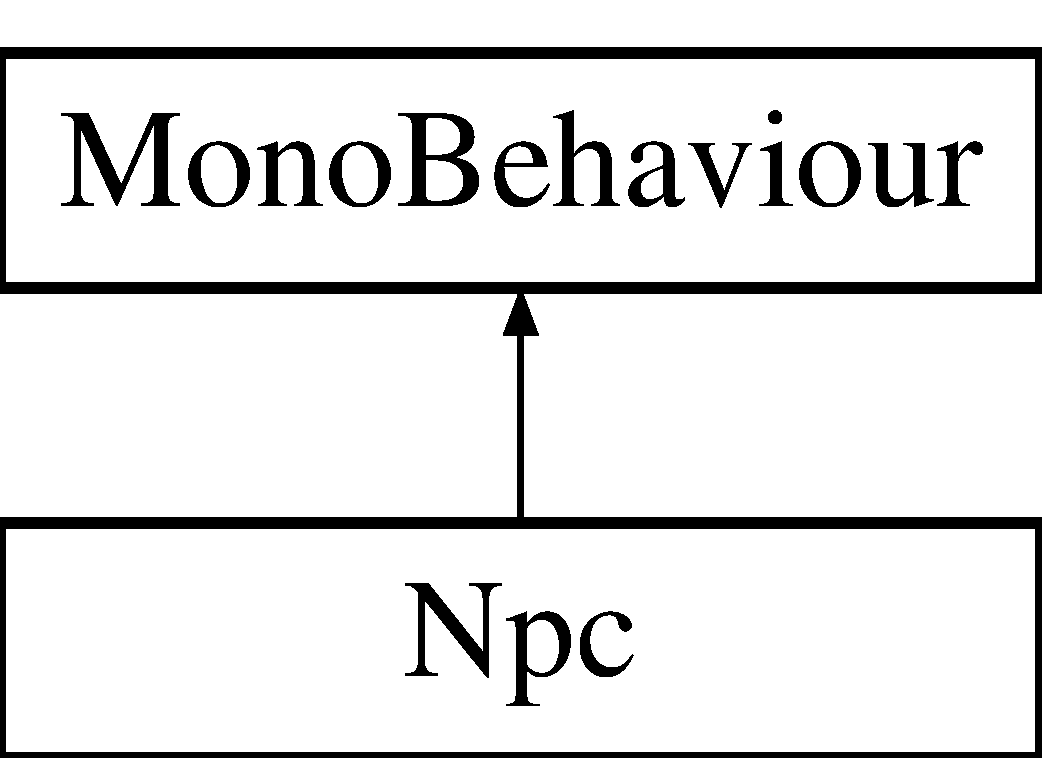
\includegraphics[height=2.000000cm]{classNpc}
\end{center}
\end{figure}
\subsection*{Public Member Functions}
\begin{DoxyCompactItemize}
\item 
bool \hyperlink{classNpc_a11e42e0b414126068d1dda54bb590c6d}{is\+Npc\+Answer\+Correct} ()
\item 
float \hyperlink{classNpc_a056b965b7212121fcb22b6db4b2567d2}{get\+Npc\+Response\+Time} ()
\item 
int \hyperlink{classNpc_a213fad208ad80e3962bffd0d1fb5e57b}{get\+Points} ()
\item 
void \hyperlink{classNpc_a9311d6bf9a43936d51656f81b706e6dc}{set\+Points} (int received\+Points)
\item 
void \hyperlink{classNpc_afc324d3e1b79722de57daf4159602f70}{set\+Mean\+Response\+Time} (int speed\+Mode)
\end{DoxyCompactItemize}


\subsection{Member Function Documentation}
\mbox{\Hypertarget{classNpc_a056b965b7212121fcb22b6db4b2567d2}\label{classNpc_a056b965b7212121fcb22b6db4b2567d2}} 
\index{Npc@{Npc}!get\+Npc\+Response\+Time@{get\+Npc\+Response\+Time}}
\index{get\+Npc\+Response\+Time@{get\+Npc\+Response\+Time}!Npc@{Npc}}
\subsubsection{\texorpdfstring{get\+Npc\+Response\+Time()}{getNpcResponseTime()}}
{\footnotesize\ttfamily float Npc.\+get\+Npc\+Response\+Time (\begin{DoxyParamCaption}{ }\end{DoxyParamCaption})\hspace{0.3cm}{\ttfamily [inline]}}

\mbox{\Hypertarget{classNpc_a213fad208ad80e3962bffd0d1fb5e57b}\label{classNpc_a213fad208ad80e3962bffd0d1fb5e57b}} 
\index{Npc@{Npc}!get\+Points@{get\+Points}}
\index{get\+Points@{get\+Points}!Npc@{Npc}}
\subsubsection{\texorpdfstring{get\+Points()}{getPoints()}}
{\footnotesize\ttfamily int Npc.\+get\+Points (\begin{DoxyParamCaption}{ }\end{DoxyParamCaption})\hspace{0.3cm}{\ttfamily [inline]}}

\mbox{\Hypertarget{classNpc_a11e42e0b414126068d1dda54bb590c6d}\label{classNpc_a11e42e0b414126068d1dda54bb590c6d}} 
\index{Npc@{Npc}!is\+Npc\+Answer\+Correct@{is\+Npc\+Answer\+Correct}}
\index{is\+Npc\+Answer\+Correct@{is\+Npc\+Answer\+Correct}!Npc@{Npc}}
\subsubsection{\texorpdfstring{is\+Npc\+Answer\+Correct()}{isNpcAnswerCorrect()}}
{\footnotesize\ttfamily bool Npc.\+is\+Npc\+Answer\+Correct (\begin{DoxyParamCaption}{ }\end{DoxyParamCaption})\hspace{0.3cm}{\ttfamily [inline]}}

\mbox{\Hypertarget{classNpc_afc324d3e1b79722de57daf4159602f70}\label{classNpc_afc324d3e1b79722de57daf4159602f70}} 
\index{Npc@{Npc}!set\+Mean\+Response\+Time@{set\+Mean\+Response\+Time}}
\index{set\+Mean\+Response\+Time@{set\+Mean\+Response\+Time}!Npc@{Npc}}
\subsubsection{\texorpdfstring{set\+Mean\+Response\+Time()}{setMeanResponseTime()}}
{\footnotesize\ttfamily void Npc.\+set\+Mean\+Response\+Time (\begin{DoxyParamCaption}\item[{int}]{speed\+Mode }\end{DoxyParamCaption})\hspace{0.3cm}{\ttfamily [inline]}}

\mbox{\Hypertarget{classNpc_a9311d6bf9a43936d51656f81b706e6dc}\label{classNpc_a9311d6bf9a43936d51656f81b706e6dc}} 
\index{Npc@{Npc}!set\+Points@{set\+Points}}
\index{set\+Points@{set\+Points}!Npc@{Npc}}
\subsubsection{\texorpdfstring{set\+Points()}{setPoints()}}
{\footnotesize\ttfamily void Npc.\+set\+Points (\begin{DoxyParamCaption}\item[{int}]{received\+Points }\end{DoxyParamCaption})\hspace{0.3cm}{\ttfamily [inline]}}



The documentation for this class was generated from the following file\+:\begin{DoxyCompactItemize}
\item 
Assets/\+Scripts/\+Balloon\+Scripts/\hyperlink{Npc_8cs}{Npc.\+cs}\end{DoxyCompactItemize}

\hypertarget{classOption}{}\section{Option Class Reference}
\label{classOption}\index{Option@{Option}}
Inheritance diagram for Option\+:\begin{figure}[H]
\begin{center}
\leavevmode
\includegraphics[height=2.000000cm]{classOption}
\end{center}
\end{figure}


The documentation for this class was generated from the following file\+:\begin{DoxyCompactItemize}
\item 
Assets/\+Scripts/\+Balloon\+Scripts/\+Component/\hyperlink{Option_8cs}{Option.\+cs}\end{DoxyCompactItemize}

\hypertarget{classPhpOutputHandler}{}\section{Php\+Output\+Handler Class Reference}
\label{classPhpOutputHandler}\index{Php\+Output\+Handler@{Php\+Output\+Handler}}
\subsection*{Public Member Functions}
\begin{DoxyCompactItemize}
\item 
\hyperlink{classPhpOutputHandler_a38a53815323031348ce5d15e0d715744}{Php\+Output\+Handler} (W\+WW result, bool verbose=false)
\item 
bool \hyperlink{classPhpOutputHandler_a4dc68556b5bc70042ce58328df9d7d98}{Success} ()
\item 
bool \hyperlink{classPhpOutputHandler_a9b04fd924fb62ad91b2da9887d917cbe}{Connection} ()
\item 
Dictionary$<$ string, string $>$ \hyperlink{classPhpOutputHandler_a0f74d89c9ae20505c5c2db462e477308}{Get\+Output} ()
\end{DoxyCompactItemize}


\subsection{Constructor \& Destructor Documentation}
\mbox{\Hypertarget{classPhpOutputHandler_a38a53815323031348ce5d15e0d715744}\label{classPhpOutputHandler_a38a53815323031348ce5d15e0d715744}} 
\index{Php\+Output\+Handler@{Php\+Output\+Handler}!Php\+Output\+Handler@{Php\+Output\+Handler}}
\index{Php\+Output\+Handler@{Php\+Output\+Handler}!Php\+Output\+Handler@{Php\+Output\+Handler}}
\subsubsection{\texorpdfstring{Php\+Output\+Handler()}{PhpOutputHandler()}}
{\footnotesize\ttfamily Php\+Output\+Handler.\+Php\+Output\+Handler (\begin{DoxyParamCaption}\item[{W\+WW}]{result,  }\item[{bool}]{verbose = {\ttfamily false} }\end{DoxyParamCaption})\hspace{0.3cm}{\ttfamily [inline]}}



\subsection{Member Function Documentation}
\mbox{\Hypertarget{classPhpOutputHandler_a9b04fd924fb62ad91b2da9887d917cbe}\label{classPhpOutputHandler_a9b04fd924fb62ad91b2da9887d917cbe}} 
\index{Php\+Output\+Handler@{Php\+Output\+Handler}!Connection@{Connection}}
\index{Connection@{Connection}!Php\+Output\+Handler@{Php\+Output\+Handler}}
\subsubsection{\texorpdfstring{Connection()}{Connection()}}
{\footnotesize\ttfamily bool Php\+Output\+Handler.\+Connection (\begin{DoxyParamCaption}{ }\end{DoxyParamCaption})\hspace{0.3cm}{\ttfamily [inline]}}

\mbox{\Hypertarget{classPhpOutputHandler_a0f74d89c9ae20505c5c2db462e477308}\label{classPhpOutputHandler_a0f74d89c9ae20505c5c2db462e477308}} 
\index{Php\+Output\+Handler@{Php\+Output\+Handler}!Get\+Output@{Get\+Output}}
\index{Get\+Output@{Get\+Output}!Php\+Output\+Handler@{Php\+Output\+Handler}}
\subsubsection{\texorpdfstring{Get\+Output()}{GetOutput()}}
{\footnotesize\ttfamily Dictionary$<$string, string$>$ Php\+Output\+Handler.\+Get\+Output (\begin{DoxyParamCaption}{ }\end{DoxyParamCaption})\hspace{0.3cm}{\ttfamily [inline]}}

\mbox{\Hypertarget{classPhpOutputHandler_a4dc68556b5bc70042ce58328df9d7d98}\label{classPhpOutputHandler_a4dc68556b5bc70042ce58328df9d7d98}} 
\index{Php\+Output\+Handler@{Php\+Output\+Handler}!Success@{Success}}
\index{Success@{Success}!Php\+Output\+Handler@{Php\+Output\+Handler}}
\subsubsection{\texorpdfstring{Success()}{Success()}}
{\footnotesize\ttfamily bool Php\+Output\+Handler.\+Success (\begin{DoxyParamCaption}{ }\end{DoxyParamCaption})\hspace{0.3cm}{\ttfamily [inline]}}



The documentation for this class was generated from the following file\+:\begin{DoxyCompactItemize}
\item 
Assets/\+Scripts/\+Misc/\hyperlink{PhpOutputHandler_8cs}{Php\+Output\+Handler.\+cs}\end{DoxyCompactItemize}

\hypertarget{classPlayer}{}\section{Player Class Reference}
\label{classPlayer}\index{Player@{Player}}
\subsection*{Public Member Functions}
\begin{DoxyCompactItemize}
\item 
\hyperlink{classPlayer_a712a726b07cf901c040116d6d0c5cc66}{Player} ()
\item 
\hyperlink{classPlayer_a1e27917f68627cae1ae9d03deb06050e}{Player} (string name)
\item 
string \hyperlink{classPlayer_a0be8a860b0f2f2345bfdb35f598064ae}{get\+Player\+Name} ()
\item 
void \hyperlink{classPlayer_a2c318642869ff9b766a5507d07b78fd3}{set\+Player\+Name} (string player\+Name)
\item 
int \hyperlink{classPlayer_ad0516b90fa518f321798b3113aec363c}{get\+Points} ()
\item 
void \hyperlink{classPlayer_a8d2d50dfbb6e990cdb52a2edaa4edd8a}{set\+Points} (int received\+Points)
\end{DoxyCompactItemize}


\subsection{Constructor \& Destructor Documentation}
\mbox{\Hypertarget{classPlayer_a712a726b07cf901c040116d6d0c5cc66}\label{classPlayer_a712a726b07cf901c040116d6d0c5cc66}} 
\index{Player@{Player}!Player@{Player}}
\index{Player@{Player}!Player@{Player}}
\subsubsection{\texorpdfstring{Player()}{Player()}\hspace{0.1cm}{\footnotesize\ttfamily [1/2]}}
{\footnotesize\ttfamily Player.\+Player (\begin{DoxyParamCaption}{ }\end{DoxyParamCaption})\hspace{0.3cm}{\ttfamily [inline]}}

\mbox{\Hypertarget{classPlayer_a1e27917f68627cae1ae9d03deb06050e}\label{classPlayer_a1e27917f68627cae1ae9d03deb06050e}} 
\index{Player@{Player}!Player@{Player}}
\index{Player@{Player}!Player@{Player}}
\subsubsection{\texorpdfstring{Player()}{Player()}\hspace{0.1cm}{\footnotesize\ttfamily [2/2]}}
{\footnotesize\ttfamily Player.\+Player (\begin{DoxyParamCaption}\item[{string}]{name }\end{DoxyParamCaption})\hspace{0.3cm}{\ttfamily [inline]}}



\subsection{Member Function Documentation}
\mbox{\Hypertarget{classPlayer_a0be8a860b0f2f2345bfdb35f598064ae}\label{classPlayer_a0be8a860b0f2f2345bfdb35f598064ae}} 
\index{Player@{Player}!get\+Player\+Name@{get\+Player\+Name}}
\index{get\+Player\+Name@{get\+Player\+Name}!Player@{Player}}
\subsubsection{\texorpdfstring{get\+Player\+Name()}{getPlayerName()}}
{\footnotesize\ttfamily string Player.\+get\+Player\+Name (\begin{DoxyParamCaption}{ }\end{DoxyParamCaption})\hspace{0.3cm}{\ttfamily [inline]}}

\mbox{\Hypertarget{classPlayer_ad0516b90fa518f321798b3113aec363c}\label{classPlayer_ad0516b90fa518f321798b3113aec363c}} 
\index{Player@{Player}!get\+Points@{get\+Points}}
\index{get\+Points@{get\+Points}!Player@{Player}}
\subsubsection{\texorpdfstring{get\+Points()}{getPoints()}}
{\footnotesize\ttfamily int Player.\+get\+Points (\begin{DoxyParamCaption}{ }\end{DoxyParamCaption})\hspace{0.3cm}{\ttfamily [inline]}}

\mbox{\Hypertarget{classPlayer_a2c318642869ff9b766a5507d07b78fd3}\label{classPlayer_a2c318642869ff9b766a5507d07b78fd3}} 
\index{Player@{Player}!set\+Player\+Name@{set\+Player\+Name}}
\index{set\+Player\+Name@{set\+Player\+Name}!Player@{Player}}
\subsubsection{\texorpdfstring{set\+Player\+Name()}{setPlayerName()}}
{\footnotesize\ttfamily void Player.\+set\+Player\+Name (\begin{DoxyParamCaption}\item[{string}]{player\+Name }\end{DoxyParamCaption})\hspace{0.3cm}{\ttfamily [inline]}}

\mbox{\Hypertarget{classPlayer_a8d2d50dfbb6e990cdb52a2edaa4edd8a}\label{classPlayer_a8d2d50dfbb6e990cdb52a2edaa4edd8a}} 
\index{Player@{Player}!set\+Points@{set\+Points}}
\index{set\+Points@{set\+Points}!Player@{Player}}
\subsubsection{\texorpdfstring{set\+Points()}{setPoints()}}
{\footnotesize\ttfamily void Player.\+set\+Points (\begin{DoxyParamCaption}\item[{int}]{received\+Points }\end{DoxyParamCaption})\hspace{0.3cm}{\ttfamily [inline]}}



The documentation for this class was generated from the following file\+:\begin{DoxyCompactItemize}
\item 
Assets/\+Scripts/\+Balloon\+Scripts/\hyperlink{Player_8cs}{Player.\+cs}\end{DoxyCompactItemize}

\hypertarget{interfaceProblem}{}\section{Problem Interface Reference}
\label{interfaceProblem}\index{Problem@{Problem}}
\subsection*{Public Member Functions}
\begin{DoxyCompactItemize}
\item 
void \hyperlink{interfaceProblem_add905385067d91a7614c1c1c57129e10}{string\+Problem\+Task} ()
\item 
void \hyperlink{interfaceProblem_a689aee9674d192aa7e67f8558a5e0925}{print\+Problem\+Solution} ()
\end{DoxyCompactItemize}


\subsection{Member Function Documentation}
\mbox{\Hypertarget{interfaceProblem_a689aee9674d192aa7e67f8558a5e0925}\label{interfaceProblem_a689aee9674d192aa7e67f8558a5e0925}} 
\index{Problem@{Problem}!print\+Problem\+Solution@{print\+Problem\+Solution}}
\index{print\+Problem\+Solution@{print\+Problem\+Solution}!Problem@{Problem}}
\subsubsection{\texorpdfstring{print\+Problem\+Solution()}{printProblemSolution()}}
{\footnotesize\ttfamily void Problem.\+print\+Problem\+Solution (\begin{DoxyParamCaption}{ }\end{DoxyParamCaption})}

\mbox{\Hypertarget{interfaceProblem_add905385067d91a7614c1c1c57129e10}\label{interfaceProblem_add905385067d91a7614c1c1c57129e10}} 
\index{Problem@{Problem}!string\+Problem\+Task@{string\+Problem\+Task}}
\index{string\+Problem\+Task@{string\+Problem\+Task}!Problem@{Problem}}
\subsubsection{\texorpdfstring{string\+Problem\+Task()}{stringProblemTask()}}
{\footnotesize\ttfamily void Problem.\+string\+Problem\+Task (\begin{DoxyParamCaption}{ }\end{DoxyParamCaption})}



The documentation for this interface was generated from the following file\+:\begin{DoxyCompactItemize}
\item 
Assets/\+Scripts/\+Balloon\+Scripts/\+Component/\hyperlink{Problem_8cs}{Problem.\+cs}\end{DoxyCompactItemize}

\hypertarget{classProjectileDragging}{}\section{Projectile\+Dragging Class Reference}
\label{classProjectileDragging}\index{Projectile\+Dragging@{Projectile\+Dragging}}
Inheritance diagram for Projectile\+Dragging\+:\begin{figure}[H]
\begin{center}
\leavevmode
\includegraphics[height=2.000000cm]{classProjectileDragging}
\end{center}
\end{figure}
\subsection*{Public Attributes}
\begin{DoxyCompactItemize}
\item 
float \hyperlink{classProjectileDragging_a543a037b4fe07cb253d6aaa519491d4b}{max\+Stretch} = 1.\+3f
\item 
float \hyperlink{classProjectileDragging_ae08a87c1eccb1c683893e66d648d2bbe}{max\+Path}
\item 
Line\+Renderer \hyperlink{classProjectileDragging_ae2b859534673bab938dcfed0e45df930}{catapult\+Line\+Left}
\item 
Line\+Renderer \hyperlink{classProjectileDragging_a1c80c1a55b8e672fe27b709af7c9cb1e}{catapult\+Line\+Right}
\item 
Line\+Renderer \hyperlink{classProjectileDragging_a2ab40fc38512c50f3ccbc00fb19aea4b}{trajectory}
\item 
Rigidbody2D \hyperlink{classProjectileDragging_a1d13cb645eb6ccb4b48d4606b83a7cf1}{player}
\end{DoxyCompactItemize}


\subsection{Member Data Documentation}
\mbox{\Hypertarget{classProjectileDragging_ae2b859534673bab938dcfed0e45df930}\label{classProjectileDragging_ae2b859534673bab938dcfed0e45df930}} 
\index{Projectile\+Dragging@{Projectile\+Dragging}!catapult\+Line\+Left@{catapult\+Line\+Left}}
\index{catapult\+Line\+Left@{catapult\+Line\+Left}!Projectile\+Dragging@{Projectile\+Dragging}}
\subsubsection{\texorpdfstring{catapult\+Line\+Left}{catapultLineLeft}}
{\footnotesize\ttfamily Line\+Renderer Projectile\+Dragging.\+catapult\+Line\+Left}

\mbox{\Hypertarget{classProjectileDragging_a1c80c1a55b8e672fe27b709af7c9cb1e}\label{classProjectileDragging_a1c80c1a55b8e672fe27b709af7c9cb1e}} 
\index{Projectile\+Dragging@{Projectile\+Dragging}!catapult\+Line\+Right@{catapult\+Line\+Right}}
\index{catapult\+Line\+Right@{catapult\+Line\+Right}!Projectile\+Dragging@{Projectile\+Dragging}}
\subsubsection{\texorpdfstring{catapult\+Line\+Right}{catapultLineRight}}
{\footnotesize\ttfamily Line\+Renderer Projectile\+Dragging.\+catapult\+Line\+Right}

\mbox{\Hypertarget{classProjectileDragging_ae08a87c1eccb1c683893e66d648d2bbe}\label{classProjectileDragging_ae08a87c1eccb1c683893e66d648d2bbe}} 
\index{Projectile\+Dragging@{Projectile\+Dragging}!max\+Path@{max\+Path}}
\index{max\+Path@{max\+Path}!Projectile\+Dragging@{Projectile\+Dragging}}
\subsubsection{\texorpdfstring{max\+Path}{maxPath}}
{\footnotesize\ttfamily float Projectile\+Dragging.\+max\+Path}

\mbox{\Hypertarget{classProjectileDragging_a543a037b4fe07cb253d6aaa519491d4b}\label{classProjectileDragging_a543a037b4fe07cb253d6aaa519491d4b}} 
\index{Projectile\+Dragging@{Projectile\+Dragging}!max\+Stretch@{max\+Stretch}}
\index{max\+Stretch@{max\+Stretch}!Projectile\+Dragging@{Projectile\+Dragging}}
\subsubsection{\texorpdfstring{max\+Stretch}{maxStretch}}
{\footnotesize\ttfamily float Projectile\+Dragging.\+max\+Stretch = 1.\+3f}

\mbox{\Hypertarget{classProjectileDragging_a1d13cb645eb6ccb4b48d4606b83a7cf1}\label{classProjectileDragging_a1d13cb645eb6ccb4b48d4606b83a7cf1}} 
\index{Projectile\+Dragging@{Projectile\+Dragging}!player@{player}}
\index{player@{player}!Projectile\+Dragging@{Projectile\+Dragging}}
\subsubsection{\texorpdfstring{player}{player}}
{\footnotesize\ttfamily Rigidbody2D Projectile\+Dragging.\+player}

\mbox{\Hypertarget{classProjectileDragging_a2ab40fc38512c50f3ccbc00fb19aea4b}\label{classProjectileDragging_a2ab40fc38512c50f3ccbc00fb19aea4b}} 
\index{Projectile\+Dragging@{Projectile\+Dragging}!trajectory@{trajectory}}
\index{trajectory@{trajectory}!Projectile\+Dragging@{Projectile\+Dragging}}
\subsubsection{\texorpdfstring{trajectory}{trajectory}}
{\footnotesize\ttfamily Line\+Renderer Projectile\+Dragging.\+trajectory}



The documentation for this class was generated from the following file\+:\begin{DoxyCompactItemize}
\item 
Assets/\+Scripts/\+Number\+Line\+Scripts/\hyperlink{ProjectileDragging_8cs}{Projectile\+Dragging.\+cs}\end{DoxyCompactItemize}

\hypertarget{classReactionData}{}\section{Reaction\+Data Class Reference}
\label{classReactionData}\index{Reaction\+Data@{Reaction\+Data}}


Provides a list of reaction data (e.\+g. time stamps) and writes it into a csv file.  




\subsection{Detailed Description}
Provides a list of reaction data (e.\+g. time stamps) and writes it into a csv file. 



The documentation for this class was generated from the following file\+:\begin{DoxyCompactItemize}
\item 
Assets/\+Scripts/\+Balloon\+Scripts/\+Component/\hyperlink{ReactionData_8cs}{Reaction\+Data.\+cs}\end{DoxyCompactItemize}

\hypertarget{classRegisterController}{}\section{Register\+Controller Class Reference}
\label{classRegisterController}\index{Register\+Controller@{Register\+Controller}}
Inheritance diagram for Register\+Controller\+:\begin{figure}[H]
\begin{center}
\leavevmode
\includegraphics[height=2.000000cm]{classRegisterController}
\end{center}
\end{figure}
\subsection*{Public Member Functions}
\begin{DoxyCompactItemize}
\item 
void \hyperlink{classRegisterController_a28f855c65269510bd5dac66aa39a1f9e}{Set\+Grade\+Dropdown\+Items} ()
\begin{DoxyCompactList}\small\item\em Sets the grade dropdown items according to the selected school. \end{DoxyCompactList}\item 
void \hyperlink{classRegisterController_a27e92b0ef5a5ba595f3b6c1a51a0c0d0}{Register\+If\+Data\+Valid} ()
\begin{DoxyCompactList}\small\item\em Check if Data in input fields of the registration form is valid and start the registration if so. \end{DoxyCompactList}\item 
void \hyperlink{classRegisterController_a6134936cccf67ed5356ebe5951ca50a8}{Registration\+Name\+Handler} (\hyperlink{classPhpOutputHandler}{Php\+Output\+Handler} handler)
\item 
void \hyperlink{classRegisterController_ac6582ef5a1dfcfedb2d84d6f31ba6f31}{Registration\+Handler} (\hyperlink{classPhpOutputHandler}{Php\+Output\+Handler} handler)
\begin{DoxyCompactList}\small\item\em Handle the php output of the registration script Proceed to login if successful, Show error message if unsuccessful \end{DoxyCompactList}\item 
void \hyperlink{classRegisterController_a607fdc380924cef70152dbb79c46d4df}{Login\+Handler} (\hyperlink{classPhpOutputHandler}{Php\+Output\+Handler} handler)
\begin{DoxyCompactList}\small\item\em Handles the php output of the login script. \end{DoxyCompactList}\item 
void \hyperlink{classRegisterController_afb9a08d203a224faee4874247d51491e}{Login} ()
\item 
bool \hyperlink{classRegisterController_a35307b8660a21bbf7a186878a50c1082}{is\+Dropdown\+Value\+Equal\+To} (Dropdown dropdown, string value)
\begin{DoxyCompactList}\small\item\em Checks if the dropdown value is equal to a given string \end{DoxyCompactList}\item 
bool \hyperlink{classRegisterController_a63d41cc83568f2a3aa0159acf51bf265}{is\+Grade\+Selected} ()
\begin{DoxyCompactList}\small\item\em Checks if the user selected the grade. \end{DoxyCompactList}\item 
bool \hyperlink{classRegisterController_a963f94012946979c3c9c85adf9f8efb9}{Has\+Email} ()
\item 
bool \hyperlink{classRegisterController_a2442b0771f689d2a974c65fd7d756874}{Has\+Age} ()
\begin{DoxyCompactList}\small\item\em Determines whether this instance has age. \end{DoxyCompactList}\item 
bool \hyperlink{classRegisterController_a6c0e18d451f9960d33d798e12c1fd6d0}{Has\+Gender} ()
\begin{DoxyCompactList}\small\item\em Determines whether this instance has sex. \end{DoxyCompactList}\item 
bool \hyperlink{classRegisterController_a9641e09116e823648addfc362af8fb24}{Has\+School\+Type} ()
\begin{DoxyCompactList}\small\item\em Determines whether this instance has school type. \end{DoxyCompactList}\item 
bool \hyperlink{classRegisterController_ace91b2c3a079dbe729ece56c3e4a1552}{Has\+Grade} ()
\begin{DoxyCompactList}\small\item\em Determines whether user selected a grade. \end{DoxyCompactList}\item 
bool \hyperlink{classRegisterController_aa5c83aee5c268b2338d29a9f1fd0282f}{Has\+State} ()
\begin{DoxyCompactList}\small\item\em Determines whether the user selected a state. \end{DoxyCompactList}\item 
bool \hyperlink{classRegisterController_ab107f3182247b1b6f62ba81278dba550}{Has\+Native\+Language} ()
\begin{DoxyCompactList}\small\item\em Determines whether the user selected a language. \end{DoxyCompactList}\item 
void \hyperlink{classRegisterController_af4daa10f24e177e3dc114128ef2aedbe}{Validate\+Email} ()
\begin{DoxyCompactList}\small\item\em Checks the email. \end{DoxyCompactList}\item 
void \hyperlink{classRegisterController_ab1addfaffc04ea9065b81724d4f7e8cb}{Validate\+Username} ()
\begin{DoxyCompactList}\small\item\em Checks the username. \end{DoxyCompactList}\item 
void \hyperlink{classRegisterController_a6ec9cefdd115c96a4619df4b4154b10b}{Validate\+Password} ()
\begin{DoxyCompactList}\small\item\em Checks if the password meets the requirements of length and containing characters \end{DoxyCompactList}\item 
void \hyperlink{classRegisterController_a0cb0ad305504222292c52f22f558822e}{Validate\+Password\+Repeat} ()
\begin{DoxyCompactList}\small\item\em Checks if the repeated password matches the password and updates the validity of the field accordingly \end{DoxyCompactList}\item 
bool \hyperlink{classRegisterController_a7728cb73673b72b2fa059200a9cbc4af}{Is\+Content\+Equal} (Input\+Field input1, Input\+Field input2)
\begin{DoxyCompactList}\small\item\em Determines whether this instance is content equal the specified input1 input2. \end{DoxyCompactList}\item 
bool \hyperlink{classRegisterController_a962585ca46ff0707c3ca32d5300c5716}{Is\+Input\+Valid} (Input\+Field input, string regex, int min\+Length, int max\+Length)
\begin{DoxyCompactList}\small\item\em Validates the input. \end{DoxyCompactList}\item 
void \hyperlink{classRegisterController_a02902491d57c7eb064bbcec47b4ff1a1}{Update\+Validity} (Input\+Field input, bool is\+Valid)
\begin{DoxyCompactList}\small\item\em Updates the validity. \end{DoxyCompactList}\item 
void \hyperlink{classRegisterController_a6a4d488534b263f16c741b920f7e3543}{Load\+Register2} ()
\item 
string \hyperlink{classRegisterController_ab69e503f3a5fbf2474abd32dad6a071f}{Get\+Username\+Login} ()
\item 
string \hyperlink{classRegisterController_a96881a003ae56e420a67436e60f27ab8}{Get\+Password\+Login} ()
\item 
string \hyperlink{classRegisterController_a9c65087784b926a7bfa3883cd7df74df}{Get\+Username} ()
\item 
string \hyperlink{classRegisterController_a3e017e31a84c05fd55855b80ee4bf082}{Get\+Email} ()
\item 
string \hyperlink{classRegisterController_a95b354b8d1933b87bcedd25994edbc3f}{Get\+Password} ()
\item 
string \hyperlink{classRegisterController_a10550f3ccac168ab1edde3e0dab6fb30}{Get\+Password\+Repeat} ()
\item 
string \hyperlink{classRegisterController_a9a6a8e029ed5a644c8fe2048b96e2121}{Get\+Age} ()
\begin{DoxyCompactList}\small\item\em Extracts the Age from the age Dropdown \end{DoxyCompactList}\item 
string \hyperlink{classRegisterController_a5b1fb947518fb240ed183733551750ab}{Get\+Gender} ()
\item 
string \hyperlink{classRegisterController_a9d045a715368cfde9b97eaacf0a2088f}{Get\+School} ()
\item 
string \hyperlink{classRegisterController_a7f1027ff167a61b09727736607bbe1a0}{Get\+Grade} ()
\item 
string \hyperlink{classRegisterController_a8f676337877ac8e82fd695c7cf7d38fb}{Get\+State} ()
\item 
string \hyperlink{classRegisterController_a5473dbdd4bf42009c9f51cb1be7b160d}{Get\+Language} ()
\end{DoxyCompactItemize}
\subsection*{Static Public Member Functions}
\begin{DoxyCompactItemize}
\item 
static string \hyperlink{classRegisterController_a3c58d07f9660dbeddd5bd41edcd4dcc3}{Get\+Selected\+Item\+From\+Dropdown} (Dropdown dropdown)
\begin{DoxyCompactList}\small\item\em Gets the selected item from dropdown. \end{DoxyCompactList}\end{DoxyCompactItemize}
\subsection*{Public Attributes}
\begin{DoxyCompactItemize}
\item 
Input\+Field \hyperlink{classRegisterController_a45cc611f9b86972779c97016a496484e}{username\+Login\+Field}
\item 
Input\+Field \hyperlink{classRegisterController_afb2904227cec3d91f80316b563c2a4d3}{password\+Login\+Field}
\item 
Input\+Field \hyperlink{classRegisterController_a47e25a3708c32d2610d8ca0db7ca51ee}{username\+Field}
\item 
Input\+Field \hyperlink{classRegisterController_a9c39e08fb93964af5d5c3c30783fa8e6}{email\+Field}
\item 
Input\+Field \hyperlink{classRegisterController_a04e4d5a4f7a00b7afeb62175455b8688}{password\+Field}
\item 
Input\+Field \hyperlink{classRegisterController_a057245e171c45f52cee78f343e7fc60c}{password\+Repeat\+Field}
\item 
Dropdown \hyperlink{classRegisterController_aa0ca4dba13add88d0bb74296ef75901c}{school\+Dropdown}
\item 
Dropdown \hyperlink{classRegisterController_af1f1c189c7974e628dd5f728a28409b6}{grade\+Dropdown}
\item 
Dropdown \hyperlink{classRegisterController_a15a9c2e4a4af0a04ded3f896eafc79a1}{day\+Dropdown}
\item 
Dropdown \hyperlink{classRegisterController_aa7fc852727ec7fc43ffe8ca7f842aee2}{month\+Dropdown}
\item 
Dropdown \hyperlink{classRegisterController_a3d0d5c6827a821305a047ac365a46fd0}{year\+Dropdown}
\item 
Dropdown \hyperlink{classRegisterController_a194e288ec2513ca13448895f95e862f9}{gender\+Dropdown}
\item 
Dropdown \hyperlink{classRegisterController_af0176c009d5aa3b397b0029473b522e9}{state\+Dropdown}
\item 
Dropdown \hyperlink{classRegisterController_a07e91bda695dab82c74e8d79ecb65f91}{language\+Dropdown}
\item 
Game\+Object \hyperlink{classRegisterController_ac81ca9cc151ce7c892f133ca5270bcb4}{login}
\item 
Game\+Object \hyperlink{classRegisterController_a8aec5b029845d59b39988246a018af8c}{register1}
\item 
Game\+Object \hyperlink{classRegisterController_a8372a097a730f83fce93fbae7531aeb5}{register2}
\end{DoxyCompactItemize}


\subsection{Member Function Documentation}
\mbox{\Hypertarget{classRegisterController_a9a6a8e029ed5a644c8fe2048b96e2121}\label{classRegisterController_a9a6a8e029ed5a644c8fe2048b96e2121}} 
\index{Register\+Controller@{Register\+Controller}!Get\+Age@{Get\+Age}}
\index{Get\+Age@{Get\+Age}!Register\+Controller@{Register\+Controller}}
\subsubsection{\texorpdfstring{Get\+Age()}{GetAge()}}
{\footnotesize\ttfamily string Register\+Controller.\+Get\+Age (\begin{DoxyParamCaption}{ }\end{DoxyParamCaption})\hspace{0.3cm}{\ttfamily [inline]}}



Extracts the Age from the age Dropdown 

\begin{DoxyReturn}{Returns}
The age.
\end{DoxyReturn}
\mbox{\Hypertarget{classRegisterController_a3e017e31a84c05fd55855b80ee4bf082}\label{classRegisterController_a3e017e31a84c05fd55855b80ee4bf082}} 
\index{Register\+Controller@{Register\+Controller}!Get\+Email@{Get\+Email}}
\index{Get\+Email@{Get\+Email}!Register\+Controller@{Register\+Controller}}
\subsubsection{\texorpdfstring{Get\+Email()}{GetEmail()}}
{\footnotesize\ttfamily string Register\+Controller.\+Get\+Email (\begin{DoxyParamCaption}{ }\end{DoxyParamCaption})\hspace{0.3cm}{\ttfamily [inline]}}

\mbox{\Hypertarget{classRegisterController_a5b1fb947518fb240ed183733551750ab}\label{classRegisterController_a5b1fb947518fb240ed183733551750ab}} 
\index{Register\+Controller@{Register\+Controller}!Get\+Gender@{Get\+Gender}}
\index{Get\+Gender@{Get\+Gender}!Register\+Controller@{Register\+Controller}}
\subsubsection{\texorpdfstring{Get\+Gender()}{GetGender()}}
{\footnotesize\ttfamily string Register\+Controller.\+Get\+Gender (\begin{DoxyParamCaption}{ }\end{DoxyParamCaption})\hspace{0.3cm}{\ttfamily [inline]}}

\mbox{\Hypertarget{classRegisterController_a7f1027ff167a61b09727736607bbe1a0}\label{classRegisterController_a7f1027ff167a61b09727736607bbe1a0}} 
\index{Register\+Controller@{Register\+Controller}!Get\+Grade@{Get\+Grade}}
\index{Get\+Grade@{Get\+Grade}!Register\+Controller@{Register\+Controller}}
\subsubsection{\texorpdfstring{Get\+Grade()}{GetGrade()}}
{\footnotesize\ttfamily string Register\+Controller.\+Get\+Grade (\begin{DoxyParamCaption}{ }\end{DoxyParamCaption})\hspace{0.3cm}{\ttfamily [inline]}}

\mbox{\Hypertarget{classRegisterController_a5473dbdd4bf42009c9f51cb1be7b160d}\label{classRegisterController_a5473dbdd4bf42009c9f51cb1be7b160d}} 
\index{Register\+Controller@{Register\+Controller}!Get\+Language@{Get\+Language}}
\index{Get\+Language@{Get\+Language}!Register\+Controller@{Register\+Controller}}
\subsubsection{\texorpdfstring{Get\+Language()}{GetLanguage()}}
{\footnotesize\ttfamily string Register\+Controller.\+Get\+Language (\begin{DoxyParamCaption}{ }\end{DoxyParamCaption})\hspace{0.3cm}{\ttfamily [inline]}}

\mbox{\Hypertarget{classRegisterController_a95b354b8d1933b87bcedd25994edbc3f}\label{classRegisterController_a95b354b8d1933b87bcedd25994edbc3f}} 
\index{Register\+Controller@{Register\+Controller}!Get\+Password@{Get\+Password}}
\index{Get\+Password@{Get\+Password}!Register\+Controller@{Register\+Controller}}
\subsubsection{\texorpdfstring{Get\+Password()}{GetPassword()}}
{\footnotesize\ttfamily string Register\+Controller.\+Get\+Password (\begin{DoxyParamCaption}{ }\end{DoxyParamCaption})\hspace{0.3cm}{\ttfamily [inline]}}

\mbox{\Hypertarget{classRegisterController_a96881a003ae56e420a67436e60f27ab8}\label{classRegisterController_a96881a003ae56e420a67436e60f27ab8}} 
\index{Register\+Controller@{Register\+Controller}!Get\+Password\+Login@{Get\+Password\+Login}}
\index{Get\+Password\+Login@{Get\+Password\+Login}!Register\+Controller@{Register\+Controller}}
\subsubsection{\texorpdfstring{Get\+Password\+Login()}{GetPasswordLogin()}}
{\footnotesize\ttfamily string Register\+Controller.\+Get\+Password\+Login (\begin{DoxyParamCaption}{ }\end{DoxyParamCaption})\hspace{0.3cm}{\ttfamily [inline]}}

\mbox{\Hypertarget{classRegisterController_a10550f3ccac168ab1edde3e0dab6fb30}\label{classRegisterController_a10550f3ccac168ab1edde3e0dab6fb30}} 
\index{Register\+Controller@{Register\+Controller}!Get\+Password\+Repeat@{Get\+Password\+Repeat}}
\index{Get\+Password\+Repeat@{Get\+Password\+Repeat}!Register\+Controller@{Register\+Controller}}
\subsubsection{\texorpdfstring{Get\+Password\+Repeat()}{GetPasswordRepeat()}}
{\footnotesize\ttfamily string Register\+Controller.\+Get\+Password\+Repeat (\begin{DoxyParamCaption}{ }\end{DoxyParamCaption})\hspace{0.3cm}{\ttfamily [inline]}}

\mbox{\Hypertarget{classRegisterController_a9d045a715368cfde9b97eaacf0a2088f}\label{classRegisterController_a9d045a715368cfde9b97eaacf0a2088f}} 
\index{Register\+Controller@{Register\+Controller}!Get\+School@{Get\+School}}
\index{Get\+School@{Get\+School}!Register\+Controller@{Register\+Controller}}
\subsubsection{\texorpdfstring{Get\+School()}{GetSchool()}}
{\footnotesize\ttfamily string Register\+Controller.\+Get\+School (\begin{DoxyParamCaption}{ }\end{DoxyParamCaption})\hspace{0.3cm}{\ttfamily [inline]}}

\mbox{\Hypertarget{classRegisterController_a3c58d07f9660dbeddd5bd41edcd4dcc3}\label{classRegisterController_a3c58d07f9660dbeddd5bd41edcd4dcc3}} 
\index{Register\+Controller@{Register\+Controller}!Get\+Selected\+Item\+From\+Dropdown@{Get\+Selected\+Item\+From\+Dropdown}}
\index{Get\+Selected\+Item\+From\+Dropdown@{Get\+Selected\+Item\+From\+Dropdown}!Register\+Controller@{Register\+Controller}}
\subsubsection{\texorpdfstring{Get\+Selected\+Item\+From\+Dropdown()}{GetSelectedItemFromDropdown()}}
{\footnotesize\ttfamily static string Register\+Controller.\+Get\+Selected\+Item\+From\+Dropdown (\begin{DoxyParamCaption}\item[{Dropdown}]{dropdown }\end{DoxyParamCaption})\hspace{0.3cm}{\ttfamily [inline]}, {\ttfamily [static]}}



Gets the selected item from dropdown. 

\begin{DoxyReturn}{Returns}
The selected item from dropdown.
\end{DoxyReturn}

\begin{DoxyParams}{Parameters}
{\em dropdown} & Dropdown.\\
\hline
\end{DoxyParams}
\mbox{\Hypertarget{classRegisterController_a8f676337877ac8e82fd695c7cf7d38fb}\label{classRegisterController_a8f676337877ac8e82fd695c7cf7d38fb}} 
\index{Register\+Controller@{Register\+Controller}!Get\+State@{Get\+State}}
\index{Get\+State@{Get\+State}!Register\+Controller@{Register\+Controller}}
\subsubsection{\texorpdfstring{Get\+State()}{GetState()}}
{\footnotesize\ttfamily string Register\+Controller.\+Get\+State (\begin{DoxyParamCaption}{ }\end{DoxyParamCaption})\hspace{0.3cm}{\ttfamily [inline]}}

\mbox{\Hypertarget{classRegisterController_a9c65087784b926a7bfa3883cd7df74df}\label{classRegisterController_a9c65087784b926a7bfa3883cd7df74df}} 
\index{Register\+Controller@{Register\+Controller}!Get\+Username@{Get\+Username}}
\index{Get\+Username@{Get\+Username}!Register\+Controller@{Register\+Controller}}
\subsubsection{\texorpdfstring{Get\+Username()}{GetUsername()}}
{\footnotesize\ttfamily string Register\+Controller.\+Get\+Username (\begin{DoxyParamCaption}{ }\end{DoxyParamCaption})\hspace{0.3cm}{\ttfamily [inline]}}

\mbox{\Hypertarget{classRegisterController_ab69e503f3a5fbf2474abd32dad6a071f}\label{classRegisterController_ab69e503f3a5fbf2474abd32dad6a071f}} 
\index{Register\+Controller@{Register\+Controller}!Get\+Username\+Login@{Get\+Username\+Login}}
\index{Get\+Username\+Login@{Get\+Username\+Login}!Register\+Controller@{Register\+Controller}}
\subsubsection{\texorpdfstring{Get\+Username\+Login()}{GetUsernameLogin()}}
{\footnotesize\ttfamily string Register\+Controller.\+Get\+Username\+Login (\begin{DoxyParamCaption}{ }\end{DoxyParamCaption})\hspace{0.3cm}{\ttfamily [inline]}}

\mbox{\Hypertarget{classRegisterController_a2442b0771f689d2a974c65fd7d756874}\label{classRegisterController_a2442b0771f689d2a974c65fd7d756874}} 
\index{Register\+Controller@{Register\+Controller}!Has\+Age@{Has\+Age}}
\index{Has\+Age@{Has\+Age}!Register\+Controller@{Register\+Controller}}
\subsubsection{\texorpdfstring{Has\+Age()}{HasAge()}}
{\footnotesize\ttfamily bool Register\+Controller.\+Has\+Age (\begin{DoxyParamCaption}{ }\end{DoxyParamCaption})\hspace{0.3cm}{\ttfamily [inline]}}



Determines whether this instance has age. 

\begin{DoxyReturn}{Returns}
{\ttfamily true} if this instance has age; otherwise, {\ttfamily false}.
\end{DoxyReturn}
\mbox{\Hypertarget{classRegisterController_a963f94012946979c3c9c85adf9f8efb9}\label{classRegisterController_a963f94012946979c3c9c85adf9f8efb9}} 
\index{Register\+Controller@{Register\+Controller}!Has\+Email@{Has\+Email}}
\index{Has\+Email@{Has\+Email}!Register\+Controller@{Register\+Controller}}
\subsubsection{\texorpdfstring{Has\+Email()}{HasEmail()}}
{\footnotesize\ttfamily bool Register\+Controller.\+Has\+Email (\begin{DoxyParamCaption}{ }\end{DoxyParamCaption})\hspace{0.3cm}{\ttfamily [inline]}}

\mbox{\Hypertarget{classRegisterController_a6c0e18d451f9960d33d798e12c1fd6d0}\label{classRegisterController_a6c0e18d451f9960d33d798e12c1fd6d0}} 
\index{Register\+Controller@{Register\+Controller}!Has\+Gender@{Has\+Gender}}
\index{Has\+Gender@{Has\+Gender}!Register\+Controller@{Register\+Controller}}
\subsubsection{\texorpdfstring{Has\+Gender()}{HasGender()}}
{\footnotesize\ttfamily bool Register\+Controller.\+Has\+Gender (\begin{DoxyParamCaption}{ }\end{DoxyParamCaption})\hspace{0.3cm}{\ttfamily [inline]}}



Determines whether this instance has sex. 

\begin{DoxyReturn}{Returns}
{\ttfamily true} if this instance has sex; otherwise, {\ttfamily false}.
\end{DoxyReturn}
\mbox{\Hypertarget{classRegisterController_ace91b2c3a079dbe729ece56c3e4a1552}\label{classRegisterController_ace91b2c3a079dbe729ece56c3e4a1552}} 
\index{Register\+Controller@{Register\+Controller}!Has\+Grade@{Has\+Grade}}
\index{Has\+Grade@{Has\+Grade}!Register\+Controller@{Register\+Controller}}
\subsubsection{\texorpdfstring{Has\+Grade()}{HasGrade()}}
{\footnotesize\ttfamily bool Register\+Controller.\+Has\+Grade (\begin{DoxyParamCaption}{ }\end{DoxyParamCaption})\hspace{0.3cm}{\ttfamily [inline]}}



Determines whether user selected a grade. 

\begin{DoxyReturn}{Returns}
{\ttfamily true} if user selected a grade; otherwise, {\ttfamily false}.
\end{DoxyReturn}
\mbox{\Hypertarget{classRegisterController_ab107f3182247b1b6f62ba81278dba550}\label{classRegisterController_ab107f3182247b1b6f62ba81278dba550}} 
\index{Register\+Controller@{Register\+Controller}!Has\+Native\+Language@{Has\+Native\+Language}}
\index{Has\+Native\+Language@{Has\+Native\+Language}!Register\+Controller@{Register\+Controller}}
\subsubsection{\texorpdfstring{Has\+Native\+Language()}{HasNativeLanguage()}}
{\footnotesize\ttfamily bool Register\+Controller.\+Has\+Native\+Language (\begin{DoxyParamCaption}{ }\end{DoxyParamCaption})\hspace{0.3cm}{\ttfamily [inline]}}



Determines whether the user selected a language. 

\begin{DoxyReturn}{Returns}
{\ttfamily true} if user selected a language; otherwise, {\ttfamily false}.
\end{DoxyReturn}
\mbox{\Hypertarget{classRegisterController_a9641e09116e823648addfc362af8fb24}\label{classRegisterController_a9641e09116e823648addfc362af8fb24}} 
\index{Register\+Controller@{Register\+Controller}!Has\+School\+Type@{Has\+School\+Type}}
\index{Has\+School\+Type@{Has\+School\+Type}!Register\+Controller@{Register\+Controller}}
\subsubsection{\texorpdfstring{Has\+School\+Type()}{HasSchoolType()}}
{\footnotesize\ttfamily bool Register\+Controller.\+Has\+School\+Type (\begin{DoxyParamCaption}{ }\end{DoxyParamCaption})\hspace{0.3cm}{\ttfamily [inline]}}



Determines whether this instance has school type. 

\begin{DoxyReturn}{Returns}
{\ttfamily true} if this instance has school type; otherwise, {\ttfamily false}.
\end{DoxyReturn}
\mbox{\Hypertarget{classRegisterController_aa5c83aee5c268b2338d29a9f1fd0282f}\label{classRegisterController_aa5c83aee5c268b2338d29a9f1fd0282f}} 
\index{Register\+Controller@{Register\+Controller}!Has\+State@{Has\+State}}
\index{Has\+State@{Has\+State}!Register\+Controller@{Register\+Controller}}
\subsubsection{\texorpdfstring{Has\+State()}{HasState()}}
{\footnotesize\ttfamily bool Register\+Controller.\+Has\+State (\begin{DoxyParamCaption}{ }\end{DoxyParamCaption})\hspace{0.3cm}{\ttfamily [inline]}}



Determines whether the user selected a state. 

\begin{DoxyReturn}{Returns}
{\ttfamily true} if user selected a state; otherwise, {\ttfamily false}.
\end{DoxyReturn}
\mbox{\Hypertarget{classRegisterController_a7728cb73673b72b2fa059200a9cbc4af}\label{classRegisterController_a7728cb73673b72b2fa059200a9cbc4af}} 
\index{Register\+Controller@{Register\+Controller}!Is\+Content\+Equal@{Is\+Content\+Equal}}
\index{Is\+Content\+Equal@{Is\+Content\+Equal}!Register\+Controller@{Register\+Controller}}
\subsubsection{\texorpdfstring{Is\+Content\+Equal()}{IsContentEqual()}}
{\footnotesize\ttfamily bool Register\+Controller.\+Is\+Content\+Equal (\begin{DoxyParamCaption}\item[{Input\+Field}]{input1,  }\item[{Input\+Field}]{input2 }\end{DoxyParamCaption})\hspace{0.3cm}{\ttfamily [inline]}}



Determines whether this instance is content equal the specified input1 input2. 

\begin{DoxyReturn}{Returns}
{\ttfamily true} if this instance is content equal the specified input1 input2; otherwise, {\ttfamily false}.
\end{DoxyReturn}

\begin{DoxyParams}{Parameters}
{\em input1} & Input1.\\
\hline
{\em input2} & Input2.\\
\hline
\end{DoxyParams}
\mbox{\Hypertarget{classRegisterController_a35307b8660a21bbf7a186878a50c1082}\label{classRegisterController_a35307b8660a21bbf7a186878a50c1082}} 
\index{Register\+Controller@{Register\+Controller}!is\+Dropdown\+Value\+Equal\+To@{is\+Dropdown\+Value\+Equal\+To}}
\index{is\+Dropdown\+Value\+Equal\+To@{is\+Dropdown\+Value\+Equal\+To}!Register\+Controller@{Register\+Controller}}
\subsubsection{\texorpdfstring{is\+Dropdown\+Value\+Equal\+To()}{isDropdownValueEqualTo()}}
{\footnotesize\ttfamily bool Register\+Controller.\+is\+Dropdown\+Value\+Equal\+To (\begin{DoxyParamCaption}\item[{Dropdown}]{dropdown,  }\item[{string}]{value }\end{DoxyParamCaption})\hspace{0.3cm}{\ttfamily [inline]}}



Checks if the dropdown value is equal to a given string 

\begin{DoxyReturn}{Returns}
{\ttfamily true}, if dropdown value equal to was ised, {\ttfamily false} otherwise.
\end{DoxyReturn}

\begin{DoxyParams}{Parameters}
{\em dropdown} & Dropdown.\\
\hline
{\em value} & Value.\\
\hline
\end{DoxyParams}
\mbox{\Hypertarget{classRegisterController_a63d41cc83568f2a3aa0159acf51bf265}\label{classRegisterController_a63d41cc83568f2a3aa0159acf51bf265}} 
\index{Register\+Controller@{Register\+Controller}!is\+Grade\+Selected@{is\+Grade\+Selected}}
\index{is\+Grade\+Selected@{is\+Grade\+Selected}!Register\+Controller@{Register\+Controller}}
\subsubsection{\texorpdfstring{is\+Grade\+Selected()}{isGradeSelected()}}
{\footnotesize\ttfamily bool Register\+Controller.\+is\+Grade\+Selected (\begin{DoxyParamCaption}{ }\end{DoxyParamCaption})\hspace{0.3cm}{\ttfamily [inline]}}



Checks if the user selected the grade. 

\begin{DoxyReturn}{Returns}
{\ttfamily true}, if grade selected was ised, {\ttfamily false} otherwise.
\end{DoxyReturn}
\mbox{\Hypertarget{classRegisterController_a962585ca46ff0707c3ca32d5300c5716}\label{classRegisterController_a962585ca46ff0707c3ca32d5300c5716}} 
\index{Register\+Controller@{Register\+Controller}!Is\+Input\+Valid@{Is\+Input\+Valid}}
\index{Is\+Input\+Valid@{Is\+Input\+Valid}!Register\+Controller@{Register\+Controller}}
\subsubsection{\texorpdfstring{Is\+Input\+Valid()}{IsInputValid()}}
{\footnotesize\ttfamily bool Register\+Controller.\+Is\+Input\+Valid (\begin{DoxyParamCaption}\item[{Input\+Field}]{input,  }\item[{string}]{regex,  }\item[{int}]{min\+Length,  }\item[{int}]{max\+Length }\end{DoxyParamCaption})\hspace{0.3cm}{\ttfamily [inline]}}



Validates the input. 

\begin{DoxyReturn}{Returns}
{\ttfamily true}, if input was validated, {\ttfamily false} otherwise.
\end{DoxyReturn}

\begin{DoxyParams}{Parameters}
{\em input} & Input.\\
\hline
{\em regex} & Regex.\\
\hline
{\em min\+Length} & Minimum length.\\
\hline
{\em max\+Length} & Max length.\\
\hline
\end{DoxyParams}
\mbox{\Hypertarget{classRegisterController_a6a4d488534b263f16c741b920f7e3543}\label{classRegisterController_a6a4d488534b263f16c741b920f7e3543}} 
\index{Register\+Controller@{Register\+Controller}!Load\+Register2@{Load\+Register2}}
\index{Load\+Register2@{Load\+Register2}!Register\+Controller@{Register\+Controller}}
\subsubsection{\texorpdfstring{Load\+Register2()}{LoadRegister2()}}
{\footnotesize\ttfamily void Register\+Controller.\+Load\+Register2 (\begin{DoxyParamCaption}{ }\end{DoxyParamCaption})\hspace{0.3cm}{\ttfamily [inline]}}

\mbox{\Hypertarget{classRegisterController_afb9a08d203a224faee4874247d51491e}\label{classRegisterController_afb9a08d203a224faee4874247d51491e}} 
\index{Register\+Controller@{Register\+Controller}!Login@{Login}}
\index{Login@{Login}!Register\+Controller@{Register\+Controller}}
\subsubsection{\texorpdfstring{Login()}{Login()}}
{\footnotesize\ttfamily void Register\+Controller.\+Login (\begin{DoxyParamCaption}{ }\end{DoxyParamCaption})\hspace{0.3cm}{\ttfamily [inline]}}

\mbox{\Hypertarget{classRegisterController_a607fdc380924cef70152dbb79c46d4df}\label{classRegisterController_a607fdc380924cef70152dbb79c46d4df}} 
\index{Register\+Controller@{Register\+Controller}!Login\+Handler@{Login\+Handler}}
\index{Login\+Handler@{Login\+Handler}!Register\+Controller@{Register\+Controller}}
\subsubsection{\texorpdfstring{Login\+Handler()}{LoginHandler()}}
{\footnotesize\ttfamily void Register\+Controller.\+Login\+Handler (\begin{DoxyParamCaption}\item[{\hyperlink{classPhpOutputHandler}{Php\+Output\+Handler}}]{handler }\end{DoxyParamCaption})\hspace{0.3cm}{\ttfamily [inline]}}



Handles the php output of the login script. 


\begin{DoxyParams}{Parameters}
{\em handler} & Handler.\\
\hline
\end{DoxyParams}
\mbox{\Hypertarget{classRegisterController_a27e92b0ef5a5ba595f3b6c1a51a0c0d0}\label{classRegisterController_a27e92b0ef5a5ba595f3b6c1a51a0c0d0}} 
\index{Register\+Controller@{Register\+Controller}!Register\+If\+Data\+Valid@{Register\+If\+Data\+Valid}}
\index{Register\+If\+Data\+Valid@{Register\+If\+Data\+Valid}!Register\+Controller@{Register\+Controller}}
\subsubsection{\texorpdfstring{Register\+If\+Data\+Valid()}{RegisterIfDataValid()}}
{\footnotesize\ttfamily void Register\+Controller.\+Register\+If\+Data\+Valid (\begin{DoxyParamCaption}{ }\end{DoxyParamCaption})\hspace{0.3cm}{\ttfamily [inline]}}



Check if Data in input fields of the registration form is valid and start the registration if so. 

\mbox{\Hypertarget{classRegisterController_ac6582ef5a1dfcfedb2d84d6f31ba6f31}\label{classRegisterController_ac6582ef5a1dfcfedb2d84d6f31ba6f31}} 
\index{Register\+Controller@{Register\+Controller}!Registration\+Handler@{Registration\+Handler}}
\index{Registration\+Handler@{Registration\+Handler}!Register\+Controller@{Register\+Controller}}
\subsubsection{\texorpdfstring{Registration\+Handler()}{RegistrationHandler()}}
{\footnotesize\ttfamily void Register\+Controller.\+Registration\+Handler (\begin{DoxyParamCaption}\item[{\hyperlink{classPhpOutputHandler}{Php\+Output\+Handler}}]{handler }\end{DoxyParamCaption})\hspace{0.3cm}{\ttfamily [inline]}}



Handle the php output of the registration script Proceed to login if successful, Show error message if unsuccessful 


\begin{DoxyParams}{Parameters}
{\em handler} & Handler.\\
\hline
\end{DoxyParams}
\mbox{\Hypertarget{classRegisterController_a6134936cccf67ed5356ebe5951ca50a8}\label{classRegisterController_a6134936cccf67ed5356ebe5951ca50a8}} 
\index{Register\+Controller@{Register\+Controller}!Registration\+Name\+Handler@{Registration\+Name\+Handler}}
\index{Registration\+Name\+Handler@{Registration\+Name\+Handler}!Register\+Controller@{Register\+Controller}}
\subsubsection{\texorpdfstring{Registration\+Name\+Handler()}{RegistrationNameHandler()}}
{\footnotesize\ttfamily void Register\+Controller.\+Registration\+Name\+Handler (\begin{DoxyParamCaption}\item[{\hyperlink{classPhpOutputHandler}{Php\+Output\+Handler}}]{handler }\end{DoxyParamCaption})\hspace{0.3cm}{\ttfamily [inline]}}

\mbox{\Hypertarget{classRegisterController_a28f855c65269510bd5dac66aa39a1f9e}\label{classRegisterController_a28f855c65269510bd5dac66aa39a1f9e}} 
\index{Register\+Controller@{Register\+Controller}!Set\+Grade\+Dropdown\+Items@{Set\+Grade\+Dropdown\+Items}}
\index{Set\+Grade\+Dropdown\+Items@{Set\+Grade\+Dropdown\+Items}!Register\+Controller@{Register\+Controller}}
\subsubsection{\texorpdfstring{Set\+Grade\+Dropdown\+Items()}{SetGradeDropdownItems()}}
{\footnotesize\ttfamily void Register\+Controller.\+Set\+Grade\+Dropdown\+Items (\begin{DoxyParamCaption}{ }\end{DoxyParamCaption})\hspace{0.3cm}{\ttfamily [inline]}}



Sets the grade dropdown items according to the selected school. 

\mbox{\Hypertarget{classRegisterController_a02902491d57c7eb064bbcec47b4ff1a1}\label{classRegisterController_a02902491d57c7eb064bbcec47b4ff1a1}} 
\index{Register\+Controller@{Register\+Controller}!Update\+Validity@{Update\+Validity}}
\index{Update\+Validity@{Update\+Validity}!Register\+Controller@{Register\+Controller}}
\subsubsection{\texorpdfstring{Update\+Validity()}{UpdateValidity()}}
{\footnotesize\ttfamily void Register\+Controller.\+Update\+Validity (\begin{DoxyParamCaption}\item[{Input\+Field}]{input,  }\item[{bool}]{is\+Valid }\end{DoxyParamCaption})\hspace{0.3cm}{\ttfamily [inline]}}



Updates the validity. 


\begin{DoxyParams}{Parameters}
{\em input} & Input.\\
\hline
{\em is\+Valid} & If set to {\ttfamily true} is valid.\\
\hline
\end{DoxyParams}
\mbox{\Hypertarget{classRegisterController_af4daa10f24e177e3dc114128ef2aedbe}\label{classRegisterController_af4daa10f24e177e3dc114128ef2aedbe}} 
\index{Register\+Controller@{Register\+Controller}!Validate\+Email@{Validate\+Email}}
\index{Validate\+Email@{Validate\+Email}!Register\+Controller@{Register\+Controller}}
\subsubsection{\texorpdfstring{Validate\+Email()}{ValidateEmail()}}
{\footnotesize\ttfamily void Register\+Controller.\+Validate\+Email (\begin{DoxyParamCaption}{ }\end{DoxyParamCaption})\hspace{0.3cm}{\ttfamily [inline]}}



Checks the email. 

\mbox{\Hypertarget{classRegisterController_a6ec9cefdd115c96a4619df4b4154b10b}\label{classRegisterController_a6ec9cefdd115c96a4619df4b4154b10b}} 
\index{Register\+Controller@{Register\+Controller}!Validate\+Password@{Validate\+Password}}
\index{Validate\+Password@{Validate\+Password}!Register\+Controller@{Register\+Controller}}
\subsubsection{\texorpdfstring{Validate\+Password()}{ValidatePassword()}}
{\footnotesize\ttfamily void Register\+Controller.\+Validate\+Password (\begin{DoxyParamCaption}{ }\end{DoxyParamCaption})\hspace{0.3cm}{\ttfamily [inline]}}



Checks if the password meets the requirements of length and containing characters 


\begin{DoxyParams}{Parameters}
{\em input} & Input.\\
\hline
\end{DoxyParams}
\mbox{\Hypertarget{classRegisterController_a0cb0ad305504222292c52f22f558822e}\label{classRegisterController_a0cb0ad305504222292c52f22f558822e}} 
\index{Register\+Controller@{Register\+Controller}!Validate\+Password\+Repeat@{Validate\+Password\+Repeat}}
\index{Validate\+Password\+Repeat@{Validate\+Password\+Repeat}!Register\+Controller@{Register\+Controller}}
\subsubsection{\texorpdfstring{Validate\+Password\+Repeat()}{ValidatePasswordRepeat()}}
{\footnotesize\ttfamily void Register\+Controller.\+Validate\+Password\+Repeat (\begin{DoxyParamCaption}{ }\end{DoxyParamCaption})\hspace{0.3cm}{\ttfamily [inline]}}



Checks if the repeated password matches the password and updates the validity of the field accordingly 


\begin{DoxyParams}{Parameters}
{\em password\+Repeat} & Password repeat.\\
\hline
\end{DoxyParams}
\mbox{\Hypertarget{classRegisterController_ab1addfaffc04ea9065b81724d4f7e8cb}\label{classRegisterController_ab1addfaffc04ea9065b81724d4f7e8cb}} 
\index{Register\+Controller@{Register\+Controller}!Validate\+Username@{Validate\+Username}}
\index{Validate\+Username@{Validate\+Username}!Register\+Controller@{Register\+Controller}}
\subsubsection{\texorpdfstring{Validate\+Username()}{ValidateUsername()}}
{\footnotesize\ttfamily void Register\+Controller.\+Validate\+Username (\begin{DoxyParamCaption}{ }\end{DoxyParamCaption})\hspace{0.3cm}{\ttfamily [inline]}}



Checks the username. 


\begin{DoxyParams}{Parameters}
{\em input} & Input.\\
\hline
\end{DoxyParams}


\subsection{Member Data Documentation}
\mbox{\Hypertarget{classRegisterController_a15a9c2e4a4af0a04ded3f896eafc79a1}\label{classRegisterController_a15a9c2e4a4af0a04ded3f896eafc79a1}} 
\index{Register\+Controller@{Register\+Controller}!day\+Dropdown@{day\+Dropdown}}
\index{day\+Dropdown@{day\+Dropdown}!Register\+Controller@{Register\+Controller}}
\subsubsection{\texorpdfstring{day\+Dropdown}{dayDropdown}}
{\footnotesize\ttfamily Dropdown Register\+Controller.\+day\+Dropdown}

\mbox{\Hypertarget{classRegisterController_a9c39e08fb93964af5d5c3c30783fa8e6}\label{classRegisterController_a9c39e08fb93964af5d5c3c30783fa8e6}} 
\index{Register\+Controller@{Register\+Controller}!email\+Field@{email\+Field}}
\index{email\+Field@{email\+Field}!Register\+Controller@{Register\+Controller}}
\subsubsection{\texorpdfstring{email\+Field}{emailField}}
{\footnotesize\ttfamily Input\+Field Register\+Controller.\+email\+Field}

\mbox{\Hypertarget{classRegisterController_a194e288ec2513ca13448895f95e862f9}\label{classRegisterController_a194e288ec2513ca13448895f95e862f9}} 
\index{Register\+Controller@{Register\+Controller}!gender\+Dropdown@{gender\+Dropdown}}
\index{gender\+Dropdown@{gender\+Dropdown}!Register\+Controller@{Register\+Controller}}
\subsubsection{\texorpdfstring{gender\+Dropdown}{genderDropdown}}
{\footnotesize\ttfamily Dropdown Register\+Controller.\+gender\+Dropdown}

\mbox{\Hypertarget{classRegisterController_af1f1c189c7974e628dd5f728a28409b6}\label{classRegisterController_af1f1c189c7974e628dd5f728a28409b6}} 
\index{Register\+Controller@{Register\+Controller}!grade\+Dropdown@{grade\+Dropdown}}
\index{grade\+Dropdown@{grade\+Dropdown}!Register\+Controller@{Register\+Controller}}
\subsubsection{\texorpdfstring{grade\+Dropdown}{gradeDropdown}}
{\footnotesize\ttfamily Dropdown Register\+Controller.\+grade\+Dropdown}

\mbox{\Hypertarget{classRegisterController_a07e91bda695dab82c74e8d79ecb65f91}\label{classRegisterController_a07e91bda695dab82c74e8d79ecb65f91}} 
\index{Register\+Controller@{Register\+Controller}!language\+Dropdown@{language\+Dropdown}}
\index{language\+Dropdown@{language\+Dropdown}!Register\+Controller@{Register\+Controller}}
\subsubsection{\texorpdfstring{language\+Dropdown}{languageDropdown}}
{\footnotesize\ttfamily Dropdown Register\+Controller.\+language\+Dropdown}

\mbox{\Hypertarget{classRegisterController_ac81ca9cc151ce7c892f133ca5270bcb4}\label{classRegisterController_ac81ca9cc151ce7c892f133ca5270bcb4}} 
\index{Register\+Controller@{Register\+Controller}!login@{login}}
\index{login@{login}!Register\+Controller@{Register\+Controller}}
\subsubsection{\texorpdfstring{login}{login}}
{\footnotesize\ttfamily Game\+Object Register\+Controller.\+login}

\mbox{\Hypertarget{classRegisterController_aa7fc852727ec7fc43ffe8ca7f842aee2}\label{classRegisterController_aa7fc852727ec7fc43ffe8ca7f842aee2}} 
\index{Register\+Controller@{Register\+Controller}!month\+Dropdown@{month\+Dropdown}}
\index{month\+Dropdown@{month\+Dropdown}!Register\+Controller@{Register\+Controller}}
\subsubsection{\texorpdfstring{month\+Dropdown}{monthDropdown}}
{\footnotesize\ttfamily Dropdown Register\+Controller.\+month\+Dropdown}

\mbox{\Hypertarget{classRegisterController_a04e4d5a4f7a00b7afeb62175455b8688}\label{classRegisterController_a04e4d5a4f7a00b7afeb62175455b8688}} 
\index{Register\+Controller@{Register\+Controller}!password\+Field@{password\+Field}}
\index{password\+Field@{password\+Field}!Register\+Controller@{Register\+Controller}}
\subsubsection{\texorpdfstring{password\+Field}{passwordField}}
{\footnotesize\ttfamily Input\+Field Register\+Controller.\+password\+Field}

\mbox{\Hypertarget{classRegisterController_afb2904227cec3d91f80316b563c2a4d3}\label{classRegisterController_afb2904227cec3d91f80316b563c2a4d3}} 
\index{Register\+Controller@{Register\+Controller}!password\+Login\+Field@{password\+Login\+Field}}
\index{password\+Login\+Field@{password\+Login\+Field}!Register\+Controller@{Register\+Controller}}
\subsubsection{\texorpdfstring{password\+Login\+Field}{passwordLoginField}}
{\footnotesize\ttfamily Input\+Field Register\+Controller.\+password\+Login\+Field}

\mbox{\Hypertarget{classRegisterController_a057245e171c45f52cee78f343e7fc60c}\label{classRegisterController_a057245e171c45f52cee78f343e7fc60c}} 
\index{Register\+Controller@{Register\+Controller}!password\+Repeat\+Field@{password\+Repeat\+Field}}
\index{password\+Repeat\+Field@{password\+Repeat\+Field}!Register\+Controller@{Register\+Controller}}
\subsubsection{\texorpdfstring{password\+Repeat\+Field}{passwordRepeatField}}
{\footnotesize\ttfamily Input\+Field Register\+Controller.\+password\+Repeat\+Field}

\mbox{\Hypertarget{classRegisterController_a8aec5b029845d59b39988246a018af8c}\label{classRegisterController_a8aec5b029845d59b39988246a018af8c}} 
\index{Register\+Controller@{Register\+Controller}!register1@{register1}}
\index{register1@{register1}!Register\+Controller@{Register\+Controller}}
\subsubsection{\texorpdfstring{register1}{register1}}
{\footnotesize\ttfamily Game\+Object Register\+Controller.\+register1}

\mbox{\Hypertarget{classRegisterController_a8372a097a730f83fce93fbae7531aeb5}\label{classRegisterController_a8372a097a730f83fce93fbae7531aeb5}} 
\index{Register\+Controller@{Register\+Controller}!register2@{register2}}
\index{register2@{register2}!Register\+Controller@{Register\+Controller}}
\subsubsection{\texorpdfstring{register2}{register2}}
{\footnotesize\ttfamily Game\+Object Register\+Controller.\+register2}

\mbox{\Hypertarget{classRegisterController_aa0ca4dba13add88d0bb74296ef75901c}\label{classRegisterController_aa0ca4dba13add88d0bb74296ef75901c}} 
\index{Register\+Controller@{Register\+Controller}!school\+Dropdown@{school\+Dropdown}}
\index{school\+Dropdown@{school\+Dropdown}!Register\+Controller@{Register\+Controller}}
\subsubsection{\texorpdfstring{school\+Dropdown}{schoolDropdown}}
{\footnotesize\ttfamily Dropdown Register\+Controller.\+school\+Dropdown}

\mbox{\Hypertarget{classRegisterController_af0176c009d5aa3b397b0029473b522e9}\label{classRegisterController_af0176c009d5aa3b397b0029473b522e9}} 
\index{Register\+Controller@{Register\+Controller}!state\+Dropdown@{state\+Dropdown}}
\index{state\+Dropdown@{state\+Dropdown}!Register\+Controller@{Register\+Controller}}
\subsubsection{\texorpdfstring{state\+Dropdown}{stateDropdown}}
{\footnotesize\ttfamily Dropdown Register\+Controller.\+state\+Dropdown}

\mbox{\Hypertarget{classRegisterController_a47e25a3708c32d2610d8ca0db7ca51ee}\label{classRegisterController_a47e25a3708c32d2610d8ca0db7ca51ee}} 
\index{Register\+Controller@{Register\+Controller}!username\+Field@{username\+Field}}
\index{username\+Field@{username\+Field}!Register\+Controller@{Register\+Controller}}
\subsubsection{\texorpdfstring{username\+Field}{usernameField}}
{\footnotesize\ttfamily Input\+Field Register\+Controller.\+username\+Field}

\mbox{\Hypertarget{classRegisterController_a45cc611f9b86972779c97016a496484e}\label{classRegisterController_a45cc611f9b86972779c97016a496484e}} 
\index{Register\+Controller@{Register\+Controller}!username\+Login\+Field@{username\+Login\+Field}}
\index{username\+Login\+Field@{username\+Login\+Field}!Register\+Controller@{Register\+Controller}}
\subsubsection{\texorpdfstring{username\+Login\+Field}{usernameLoginField}}
{\footnotesize\ttfamily Input\+Field Register\+Controller.\+username\+Login\+Field}

\mbox{\Hypertarget{classRegisterController_a3d0d5c6827a821305a047ac365a46fd0}\label{classRegisterController_a3d0d5c6827a821305a047ac365a46fd0}} 
\index{Register\+Controller@{Register\+Controller}!year\+Dropdown@{year\+Dropdown}}
\index{year\+Dropdown@{year\+Dropdown}!Register\+Controller@{Register\+Controller}}
\subsubsection{\texorpdfstring{year\+Dropdown}{yearDropdown}}
{\footnotesize\ttfamily Dropdown Register\+Controller.\+year\+Dropdown}



The documentation for this class was generated from the following file\+:\begin{DoxyCompactItemize}
\item 
Assets/\+Scripts/\hyperlink{RegisterController_8cs}{Register\+Controller.\+cs}\end{DoxyCompactItemize}

\hypertarget{classScrollRectSnap}{}\section{Scroll\+Rect\+Snap Class Reference}
\label{classScrollRectSnap}\index{Scroll\+Rect\+Snap@{Scroll\+Rect\+Snap}}
Inheritance diagram for Scroll\+Rect\+Snap\+:\begin{figure}[H]
\begin{center}
\leavevmode
\includegraphics[height=2.000000cm]{classScrollRectSnap}
\end{center}
\end{figure}
\subsection*{Public Member Functions}
\begin{DoxyCompactItemize}
\item 
void \hyperlink{classScrollRectSnap_ac30957c07a9f81edc4acafdb65600d27}{Start\+Drag} ()
\item 
void \hyperlink{classScrollRectSnap_aa3fbbad35f3f144e2ce508ab06a781ce}{End\+Drag} ()
\end{DoxyCompactItemize}
\subsection*{Public Attributes}
\begin{DoxyCompactItemize}
\item 
Rect\+Transform \hyperlink{classScrollRectSnap_a79161928f3a343aa90dd4d552bf7a7d7}{panel}
\item 
Button \mbox{[}$\,$\mbox{]} \hyperlink{classScrollRectSnap_abe4149dd4a42500fbdd321b2c4471322}{buttons}
\item 
Rect\+Transform \hyperlink{classScrollRectSnap_a0af76cd3bbe9c69b6482fedfd04e6f5a}{center}
\item 
float \mbox{[}$\,$\mbox{]} \hyperlink{classScrollRectSnap_a6956e26eab23ba0e943fc31ebfc48b9e}{distance}
\end{DoxyCompactItemize}


\subsection{Member Function Documentation}
\mbox{\Hypertarget{classScrollRectSnap_aa3fbbad35f3f144e2ce508ab06a781ce}\label{classScrollRectSnap_aa3fbbad35f3f144e2ce508ab06a781ce}} 
\index{Scroll\+Rect\+Snap@{Scroll\+Rect\+Snap}!End\+Drag@{End\+Drag}}
\index{End\+Drag@{End\+Drag}!Scroll\+Rect\+Snap@{Scroll\+Rect\+Snap}}
\subsubsection{\texorpdfstring{End\+Drag()}{EndDrag()}}
{\footnotesize\ttfamily void Scroll\+Rect\+Snap.\+End\+Drag (\begin{DoxyParamCaption}{ }\end{DoxyParamCaption})\hspace{0.3cm}{\ttfamily [inline]}}

\mbox{\Hypertarget{classScrollRectSnap_ac30957c07a9f81edc4acafdb65600d27}\label{classScrollRectSnap_ac30957c07a9f81edc4acafdb65600d27}} 
\index{Scroll\+Rect\+Snap@{Scroll\+Rect\+Snap}!Start\+Drag@{Start\+Drag}}
\index{Start\+Drag@{Start\+Drag}!Scroll\+Rect\+Snap@{Scroll\+Rect\+Snap}}
\subsubsection{\texorpdfstring{Start\+Drag()}{StartDrag()}}
{\footnotesize\ttfamily void Scroll\+Rect\+Snap.\+Start\+Drag (\begin{DoxyParamCaption}{ }\end{DoxyParamCaption})\hspace{0.3cm}{\ttfamily [inline]}}



\subsection{Member Data Documentation}
\mbox{\Hypertarget{classScrollRectSnap_abe4149dd4a42500fbdd321b2c4471322}\label{classScrollRectSnap_abe4149dd4a42500fbdd321b2c4471322}} 
\index{Scroll\+Rect\+Snap@{Scroll\+Rect\+Snap}!buttons@{buttons}}
\index{buttons@{buttons}!Scroll\+Rect\+Snap@{Scroll\+Rect\+Snap}}
\subsubsection{\texorpdfstring{buttons}{buttons}}
{\footnotesize\ttfamily Button \mbox{[}$\,$\mbox{]} Scroll\+Rect\+Snap.\+buttons}

\mbox{\Hypertarget{classScrollRectSnap_a0af76cd3bbe9c69b6482fedfd04e6f5a}\label{classScrollRectSnap_a0af76cd3bbe9c69b6482fedfd04e6f5a}} 
\index{Scroll\+Rect\+Snap@{Scroll\+Rect\+Snap}!center@{center}}
\index{center@{center}!Scroll\+Rect\+Snap@{Scroll\+Rect\+Snap}}
\subsubsection{\texorpdfstring{center}{center}}
{\footnotesize\ttfamily Rect\+Transform Scroll\+Rect\+Snap.\+center}

\mbox{\Hypertarget{classScrollRectSnap_a6956e26eab23ba0e943fc31ebfc48b9e}\label{classScrollRectSnap_a6956e26eab23ba0e943fc31ebfc48b9e}} 
\index{Scroll\+Rect\+Snap@{Scroll\+Rect\+Snap}!distance@{distance}}
\index{distance@{distance}!Scroll\+Rect\+Snap@{Scroll\+Rect\+Snap}}
\subsubsection{\texorpdfstring{distance}{distance}}
{\footnotesize\ttfamily float \mbox{[}$\,$\mbox{]} Scroll\+Rect\+Snap.\+distance}

\mbox{\Hypertarget{classScrollRectSnap_a79161928f3a343aa90dd4d552bf7a7d7}\label{classScrollRectSnap_a79161928f3a343aa90dd4d552bf7a7d7}} 
\index{Scroll\+Rect\+Snap@{Scroll\+Rect\+Snap}!panel@{panel}}
\index{panel@{panel}!Scroll\+Rect\+Snap@{Scroll\+Rect\+Snap}}
\subsubsection{\texorpdfstring{panel}{panel}}
{\footnotesize\ttfamily Rect\+Transform Scroll\+Rect\+Snap.\+panel}



The documentation for this class was generated from the following file\+:\begin{DoxyCompactItemize}
\item 
Assets/\+Scripts/\hyperlink{ScrollRectSnap_8cs}{Scroll\+Rect\+Snap.\+cs}\end{DoxyCompactItemize}

\hypertarget{classTestLine1}{}\section{Test\+Line1 Class Reference}
\label{classTestLine1}\index{Test\+Line1@{Test\+Line1}}
Inheritance diagram for Test\+Line1\+:\begin{figure}[H]
\begin{center}
\leavevmode
\includegraphics[height=2.000000cm]{classTestLine1}
\end{center}
\end{figure}
\subsection*{Public Attributes}
\begin{DoxyCompactItemize}
\item 
Text \hyperlink{classTestLine1_a21289056dbe86698df6cc609da19194e}{random\+Number\+Text}
\item 
Text \hyperlink{classTestLine1_a2074231e648b0dbb0ec7c8569837370a}{minimum\+Text}
\item 
Text \hyperlink{classTestLine1_ad1476ffb63c9b53642a9f27d2619f5f3}{maximum\+Text}
\item 
Text \hyperlink{classTestLine1_ac3d1f6d386ed0eb304eb18e8c872c8a5}{Result\+Text}
\item 
Rigidbody2D \hyperlink{classTestLine1_a79bfe38a9b618f57d2335289f170a819}{player}
\item 
Game\+Object \hyperlink{classTestLine1_a6099bcd6bb6ce98f49fdebf5b346d3b7}{explosion}
\item 
Game\+Object \hyperlink{classTestLine1_af9c1263870a0427ad6aa88c486e6367c}{arrow}
\item 
float \hyperlink{classTestLine1_a942aca198616b990c7bfd729e17659da}{minimum}
\item 
float \hyperlink{classTestLine1_a35ee62dc1f40b32c57b4652f036c41df}{maximum}
\item 
int \hyperlink{classTestLine1_a533c8bc73c48db7b94b0a4b98ac2e307}{trials}
\item 
int \mbox{[}$\,$\mbox{]} \hyperlink{classTestLine1_a7f5d0d4f0922b32d920f349ac3a28f0e}{target}
\end{DoxyCompactItemize}


\subsection{Member Data Documentation}
\mbox{\Hypertarget{classTestLine1_af9c1263870a0427ad6aa88c486e6367c}\label{classTestLine1_af9c1263870a0427ad6aa88c486e6367c}} 
\index{Test\+Line1@{Test\+Line1}!arrow@{arrow}}
\index{arrow@{arrow}!Test\+Line1@{Test\+Line1}}
\subsubsection{\texorpdfstring{arrow}{arrow}}
{\footnotesize\ttfamily Game\+Object Test\+Line1.\+arrow}

\mbox{\Hypertarget{classTestLine1_a6099bcd6bb6ce98f49fdebf5b346d3b7}\label{classTestLine1_a6099bcd6bb6ce98f49fdebf5b346d3b7}} 
\index{Test\+Line1@{Test\+Line1}!explosion@{explosion}}
\index{explosion@{explosion}!Test\+Line1@{Test\+Line1}}
\subsubsection{\texorpdfstring{explosion}{explosion}}
{\footnotesize\ttfamily Game\+Object Test\+Line1.\+explosion}

\mbox{\Hypertarget{classTestLine1_a35ee62dc1f40b32c57b4652f036c41df}\label{classTestLine1_a35ee62dc1f40b32c57b4652f036c41df}} 
\index{Test\+Line1@{Test\+Line1}!maximum@{maximum}}
\index{maximum@{maximum}!Test\+Line1@{Test\+Line1}}
\subsubsection{\texorpdfstring{maximum}{maximum}}
{\footnotesize\ttfamily float Test\+Line1.\+maximum}

\mbox{\Hypertarget{classTestLine1_ad1476ffb63c9b53642a9f27d2619f5f3}\label{classTestLine1_ad1476ffb63c9b53642a9f27d2619f5f3}} 
\index{Test\+Line1@{Test\+Line1}!maximum\+Text@{maximum\+Text}}
\index{maximum\+Text@{maximum\+Text}!Test\+Line1@{Test\+Line1}}
\subsubsection{\texorpdfstring{maximum\+Text}{maximumText}}
{\footnotesize\ttfamily Text Test\+Line1.\+maximum\+Text}

\mbox{\Hypertarget{classTestLine1_a942aca198616b990c7bfd729e17659da}\label{classTestLine1_a942aca198616b990c7bfd729e17659da}} 
\index{Test\+Line1@{Test\+Line1}!minimum@{minimum}}
\index{minimum@{minimum}!Test\+Line1@{Test\+Line1}}
\subsubsection{\texorpdfstring{minimum}{minimum}}
{\footnotesize\ttfamily float Test\+Line1.\+minimum}

\mbox{\Hypertarget{classTestLine1_a2074231e648b0dbb0ec7c8569837370a}\label{classTestLine1_a2074231e648b0dbb0ec7c8569837370a}} 
\index{Test\+Line1@{Test\+Line1}!minimum\+Text@{minimum\+Text}}
\index{minimum\+Text@{minimum\+Text}!Test\+Line1@{Test\+Line1}}
\subsubsection{\texorpdfstring{minimum\+Text}{minimumText}}
{\footnotesize\ttfamily Text Test\+Line1.\+minimum\+Text}

\mbox{\Hypertarget{classTestLine1_a79bfe38a9b618f57d2335289f170a819}\label{classTestLine1_a79bfe38a9b618f57d2335289f170a819}} 
\index{Test\+Line1@{Test\+Line1}!player@{player}}
\index{player@{player}!Test\+Line1@{Test\+Line1}}
\subsubsection{\texorpdfstring{player}{player}}
{\footnotesize\ttfamily Rigidbody2D Test\+Line1.\+player}

\mbox{\Hypertarget{classTestLine1_a21289056dbe86698df6cc609da19194e}\label{classTestLine1_a21289056dbe86698df6cc609da19194e}} 
\index{Test\+Line1@{Test\+Line1}!random\+Number\+Text@{random\+Number\+Text}}
\index{random\+Number\+Text@{random\+Number\+Text}!Test\+Line1@{Test\+Line1}}
\subsubsection{\texorpdfstring{random\+Number\+Text}{randomNumberText}}
{\footnotesize\ttfamily Text Test\+Line1.\+random\+Number\+Text}

\mbox{\Hypertarget{classTestLine1_ac3d1f6d386ed0eb304eb18e8c872c8a5}\label{classTestLine1_ac3d1f6d386ed0eb304eb18e8c872c8a5}} 
\index{Test\+Line1@{Test\+Line1}!Result\+Text@{Result\+Text}}
\index{Result\+Text@{Result\+Text}!Test\+Line1@{Test\+Line1}}
\subsubsection{\texorpdfstring{Result\+Text}{ResultText}}
{\footnotesize\ttfamily Text Test\+Line1.\+Result\+Text}

\mbox{\Hypertarget{classTestLine1_a7f5d0d4f0922b32d920f349ac3a28f0e}\label{classTestLine1_a7f5d0d4f0922b32d920f349ac3a28f0e}} 
\index{Test\+Line1@{Test\+Line1}!target@{target}}
\index{target@{target}!Test\+Line1@{Test\+Line1}}
\subsubsection{\texorpdfstring{target}{target}}
{\footnotesize\ttfamily int \mbox{[}$\,$\mbox{]} Test\+Line1.\+target}

\mbox{\Hypertarget{classTestLine1_a533c8bc73c48db7b94b0a4b98ac2e307}\label{classTestLine1_a533c8bc73c48db7b94b0a4b98ac2e307}} 
\index{Test\+Line1@{Test\+Line1}!trials@{trials}}
\index{trials@{trials}!Test\+Line1@{Test\+Line1}}
\subsubsection{\texorpdfstring{trials}{trials}}
{\footnotesize\ttfamily int Test\+Line1.\+trials}



The documentation for this class was generated from the following file\+:\begin{DoxyCompactItemize}
\item 
Assets/\+Scripts/\+Number\+Line\+Scripts/\hyperlink{TestLine1_8cs}{Test\+Line1.\+cs}\end{DoxyCompactItemize}

\hypertarget{classTimeStamp}{}\section{Time\+Stamp Class Reference}
\label{classTimeStamp}\index{Time\+Stamp@{Time\+Stamp}}
\subsection*{Public Member Functions}
\begin{DoxyCompactItemize}
\item 
\hyperlink{classTimeStamp_ae9ffa3706d19523c5fe43e23fe436f8d}{Time\+Stamp} (Date\+Time action\+Time, string action\+Mode)
\item 
Date\+Time \hyperlink{classTimeStamp_a10a14e554b1fa549ac6b19edbdd3179c}{get\+Action\+Time} ()
\item 
string \hyperlink{classTimeStamp_ad30b4576e73772cd5ad15ff6174d5c99}{get\+Action\+Mode} ()
\end{DoxyCompactItemize}


\subsection{Constructor \& Destructor Documentation}
\mbox{\Hypertarget{classTimeStamp_ae9ffa3706d19523c5fe43e23fe436f8d}\label{classTimeStamp_ae9ffa3706d19523c5fe43e23fe436f8d}} 
\index{Time\+Stamp@{Time\+Stamp}!Time\+Stamp@{Time\+Stamp}}
\index{Time\+Stamp@{Time\+Stamp}!Time\+Stamp@{Time\+Stamp}}
\subsubsection{\texorpdfstring{Time\+Stamp()}{TimeStamp()}}
{\footnotesize\ttfamily Time\+Stamp.\+Time\+Stamp (\begin{DoxyParamCaption}\item[{Date\+Time}]{action\+Time,  }\item[{string}]{action\+Mode }\end{DoxyParamCaption})\hspace{0.3cm}{\ttfamily [inline]}}



\subsection{Member Function Documentation}
\mbox{\Hypertarget{classTimeStamp_ad30b4576e73772cd5ad15ff6174d5c99}\label{classTimeStamp_ad30b4576e73772cd5ad15ff6174d5c99}} 
\index{Time\+Stamp@{Time\+Stamp}!get\+Action\+Mode@{get\+Action\+Mode}}
\index{get\+Action\+Mode@{get\+Action\+Mode}!Time\+Stamp@{Time\+Stamp}}
\subsubsection{\texorpdfstring{get\+Action\+Mode()}{getActionMode()}}
{\footnotesize\ttfamily string Time\+Stamp.\+get\+Action\+Mode (\begin{DoxyParamCaption}{ }\end{DoxyParamCaption})\hspace{0.3cm}{\ttfamily [inline]}}

\mbox{\Hypertarget{classTimeStamp_a10a14e554b1fa549ac6b19edbdd3179c}\label{classTimeStamp_a10a14e554b1fa549ac6b19edbdd3179c}} 
\index{Time\+Stamp@{Time\+Stamp}!get\+Action\+Time@{get\+Action\+Time}}
\index{get\+Action\+Time@{get\+Action\+Time}!Time\+Stamp@{Time\+Stamp}}
\subsubsection{\texorpdfstring{get\+Action\+Time()}{getActionTime()}}
{\footnotesize\ttfamily Date\+Time Time\+Stamp.\+get\+Action\+Time (\begin{DoxyParamCaption}{ }\end{DoxyParamCaption})\hspace{0.3cm}{\ttfamily [inline]}}



The documentation for this class was generated from the following file\+:\begin{DoxyCompactItemize}
\item 
Assets/\+Scripts/\+Balloon\+Scripts/\+Component/\hyperlink{TimeStamp_8cs}{Time\+Stamp.\+cs}\end{DoxyCompactItemize}

\hypertarget{classTooltip}{}\section{Tooltip Class Reference}
\label{classTooltip}\index{Tooltip@{Tooltip}}
Inheritance diagram for Tooltip\+:\begin{figure}[H]
\begin{center}
\leavevmode
\includegraphics[height=2.000000cm]{classTooltip}
\end{center}
\end{figure}
\subsection*{Public Member Functions}
\begin{DoxyCompactItemize}
\item 
void \hyperlink{classTooltip_aa3f2576744ee716d7e410d31e8c2015a}{Hide} ()
\item 
void \hyperlink{classTooltip_ad15715a262e1c7c27db36cba7da3149f}{Show} ()
\end{DoxyCompactItemize}
\subsection*{Public Attributes}
\begin{DoxyCompactItemize}
\item 
Game\+Object \hyperlink{classTooltip_a9e16563f3ea6f787045747f3bbc9cf9e}{tooltip\+Prefab}
\item 
Game\+Object \hyperlink{classTooltip_a58db06fa78d7d032bee7492976b4465c}{tooltip\+Parent}
\item 
string \hyperlink{classTooltip_ae1fbc466dbee2cd63d8b68df52f5b284}{tooltip\+Text}
\end{DoxyCompactItemize}


\subsection{Member Function Documentation}
\mbox{\Hypertarget{classTooltip_aa3f2576744ee716d7e410d31e8c2015a}\label{classTooltip_aa3f2576744ee716d7e410d31e8c2015a}} 
\index{Tooltip@{Tooltip}!Hide@{Hide}}
\index{Hide@{Hide}!Tooltip@{Tooltip}}
\subsubsection{\texorpdfstring{Hide()}{Hide()}}
{\footnotesize\ttfamily void Tooltip.\+Hide (\begin{DoxyParamCaption}{ }\end{DoxyParamCaption})\hspace{0.3cm}{\ttfamily [inline]}}

\mbox{\Hypertarget{classTooltip_ad15715a262e1c7c27db36cba7da3149f}\label{classTooltip_ad15715a262e1c7c27db36cba7da3149f}} 
\index{Tooltip@{Tooltip}!Show@{Show}}
\index{Show@{Show}!Tooltip@{Tooltip}}
\subsubsection{\texorpdfstring{Show()}{Show()}}
{\footnotesize\ttfamily void Tooltip.\+Show (\begin{DoxyParamCaption}{ }\end{DoxyParamCaption})\hspace{0.3cm}{\ttfamily [inline]}}



\subsection{Member Data Documentation}
\mbox{\Hypertarget{classTooltip_a58db06fa78d7d032bee7492976b4465c}\label{classTooltip_a58db06fa78d7d032bee7492976b4465c}} 
\index{Tooltip@{Tooltip}!tooltip\+Parent@{tooltip\+Parent}}
\index{tooltip\+Parent@{tooltip\+Parent}!Tooltip@{Tooltip}}
\subsubsection{\texorpdfstring{tooltip\+Parent}{tooltipParent}}
{\footnotesize\ttfamily Game\+Object Tooltip.\+tooltip\+Parent}

\mbox{\Hypertarget{classTooltip_a9e16563f3ea6f787045747f3bbc9cf9e}\label{classTooltip_a9e16563f3ea6f787045747f3bbc9cf9e}} 
\index{Tooltip@{Tooltip}!tooltip\+Prefab@{tooltip\+Prefab}}
\index{tooltip\+Prefab@{tooltip\+Prefab}!Tooltip@{Tooltip}}
\subsubsection{\texorpdfstring{tooltip\+Prefab}{tooltipPrefab}}
{\footnotesize\ttfamily Game\+Object Tooltip.\+tooltip\+Prefab}

\mbox{\Hypertarget{classTooltip_ae1fbc466dbee2cd63d8b68df52f5b284}\label{classTooltip_ae1fbc466dbee2cd63d8b68df52f5b284}} 
\index{Tooltip@{Tooltip}!tooltip\+Text@{tooltip\+Text}}
\index{tooltip\+Text@{tooltip\+Text}!Tooltip@{Tooltip}}
\subsubsection{\texorpdfstring{tooltip\+Text}{tooltipText}}
{\footnotesize\ttfamily string Tooltip.\+tooltip\+Text}



The documentation for this class was generated from the following file\+:\begin{DoxyCompactItemize}
\item 
Assets/\+Scripts/\+Tooltip/\hyperlink{Tooltip_8cs}{Tooltip.\+cs}\end{DoxyCompactItemize}

\hypertarget{classView}{}\section{View Class Reference}
\label{classView}\index{View@{View}}
Inheritance diagram for View\+:\begin{figure}[H]
\begin{center}
\leavevmode
\includegraphics[height=2.000000cm]{classView}
\end{center}
\end{figure}
\subsection*{Public Member Functions}
\begin{DoxyCompactItemize}
\item 
\hyperlink{classView_a218e935db0c3320275ff8a56637d2f47}{View} ()
\item 
void \hyperlink{classView_ade124fb0c6d19ad9c4ff64f58b37d13b}{set\+Player\+Name} (string player\+Name)
\item 
void \hyperlink{classView_a6d8bb240232381d2018d3b26393b51c0}{set\+Disabled\+Button\+Color} (Button button, Color color)
\item 
void \hyperlink{classView_a979f3676bda4ef9f79bcf5b601120c9a}{update\+Score\+Display} (int new\+Points, bool is\+Player)
\item 
void \hyperlink{classView_aa0b0a3a9e4ae68745de1870b4f85433e}{set\+Button\+Texts} (Array\+List options)
\item 
void \hyperlink{classView_a6fd402a60f74017d20a321e05d8bc787}{set\+Task\+Text} (string task)
\item 
void \hyperlink{classView_a8586560027cd5d93aaf70d494c0189b4}{reset\+All\+Buttons} ()
\item 
void \hyperlink{classView_a89b76b661b1bb6511d4b86ff3cf6a0b0}{disable\+All\+Buttons} ()
\item 
void \hyperlink{classView_a9707ef8cbbb82f46263230d2623716eb}{make\+Balloon\+Main\+Invisible} (int i)
\item 
void \hyperlink{classView_a34ea9f566a24a298d6848c497438ca9d}{make\+Balloon\+Main\+Visible} (int i)
\item 
void \hyperlink{classView_a7b8dc6ece898af6cce44d1b48e1d1ccd}{pop\+Balloon} (int i, Color color)
\item 
void \hyperlink{classView_a827b596956e88fd616050dcdd0dee6d2}{let\+Balloon\+Fly\+Away} (int i)
\item 
void \hyperlink{classView_a1ce5325961058c28aeb0d31cf8e8dfa1}{pop\+Balloon\+Except\+Index} (int index, Color color)
\item 
void \hyperlink{classView_a311fc84582f2dcb23dfbc77dcf5f82e3}{let\+Ballons\+Fly\+Away\+Except\+Index} (int index)
\item 
void \hyperlink{classView_a00bad032ce14da298bf9ab08fe13fd35}{reset\+All\+Balloons} ()
\end{DoxyCompactItemize}
\subsection*{Public Attributes}
\begin{DoxyCompactItemize}
\item 
Button \hyperlink{classView_ab24c89ecf477d77b956221a7b24976d5}{button0}
\item 
Button \hyperlink{classView_aee755ead44f4386d3cafd0c3aec5f4fb}{button1}
\item 
Button \hyperlink{classView_a63910e46c76f43286b5a761de47a3aeb}{button2}
\item 
Button \hyperlink{classView_ab330218dd82658f3abe34d3fea5c2fab}{button3}
\item 
Button \hyperlink{classView_a249b9c2451b7fbf9d969c5f3e1fbdfc4}{button4}
\item 
Button \hyperlink{classView_ae3a6abfbc84463714aa3144c12c38ba4}{button5}
\item 
Button \hyperlink{classView_ac55a000c8304cc86df581fe78c7eb08e}{button6}
\item 
Button \hyperlink{classView_a56874d01e74b8a37e0019ce81ce5c8ed}{button7}
\item 
Button \hyperlink{classView_a7fe9a1e5d0ef962a54e00fe4b7815c1b}{button8}
\item 
Game\+Object \hyperlink{classView_aaa0f9d99fe29ef9a4eba300d45feeabe}{balloon\+Main0}
\item 
Game\+Object \hyperlink{classView_a5d188e31ed902ed3968533f884dca9f5}{balloon\+Main1}
\item 
Game\+Object \hyperlink{classView_a67500752a0337243ac0e3eadd5f310b3}{balloon\+Main2}
\item 
Game\+Object \hyperlink{classView_a3d8319d6190dc2c8fba42a5beabc473a}{balloon\+Main3}
\item 
Game\+Object \hyperlink{classView_a88448abb2beed073ba07cbe9c2e1b2a1}{balloon\+Main4}
\item 
Game\+Object \hyperlink{classView_a2b6770bc88911285178e85df8c8217cc}{balloon\+Main5}
\item 
Game\+Object \hyperlink{classView_a4f9376e09967c775e3a195c85b7ab2ca}{balloon\+Main6}
\item 
Game\+Object \hyperlink{classView_a94dac7f0bcd5897db614c2ee6632c6fc}{balloon\+Main7}
\item 
Game\+Object \hyperlink{classView_aef99e7ebac1c186e6d689290970bd29e}{balloon\+Main8}
\item 
List$<$ Button $>$ \hyperlink{classView_a43cf4c0712a5ee52704dd6a0c2dd1ae3}{button\+List} = new List$<$Button$>$()
\item 
List$<$ Game\+Object $>$ \hyperlink{classView_a7e98040704d8238e9a2002d9a6ad8971}{balloon\+Main\+List} = new List$<$Game\+Object$>$()
\item 
List$<$ Vector3 $>$ \hyperlink{classView_ad4d9a01ca0600eca1bbb2304399de812}{balloon\+Position\+List} = new List$<$Vector3$>$()
\item 
Text \hyperlink{classView_a046ed9689af065a613d9bc169952b6ea}{task\+Text}
\item 
Text \hyperlink{classView_a9743e2966354094f2078593bc04c64e3}{player\+Score\+Text}
\item 
Text \hyperlink{classView_aef06655ff7a3a1af1fa1df035e147324}{player\+Name\+Text}
\item 
Text \hyperlink{classView_a824504d7a36642711e793df9b5de12b6}{npc\+Score\+Text}
\item 
Color \hyperlink{classView_a2e814ae916d1d796691e15899af94940}{c\+Wrong} = Color.\+gray
\item 
Color \hyperlink{classView_a5f3012dbcce0ef379184c6e672d8fd5d}{c\+Right} = Color.\+white
\item 
Audio\+Source \hyperlink{classView_a953e9a636c7a299f8d367caf25f1e030}{balloon\+Popping\+Sound}
\item 
\hyperlink{classNavigationSystem}{Navigation\+System} \hyperlink{classView_a983ba5bf73850b60e7a45b50c7a1d776}{navigation\+System}
\end{DoxyCompactItemize}


\subsection{Constructor \& Destructor Documentation}
\mbox{\Hypertarget{classView_a218e935db0c3320275ff8a56637d2f47}\label{classView_a218e935db0c3320275ff8a56637d2f47}} 
\index{View@{View}!View@{View}}
\index{View@{View}!View@{View}}
\subsubsection{\texorpdfstring{View()}{View()}}
{\footnotesize\ttfamily View.\+View (\begin{DoxyParamCaption}{ }\end{DoxyParamCaption})\hspace{0.3cm}{\ttfamily [inline]}}



\subsection{Member Function Documentation}
\mbox{\Hypertarget{classView_a89b76b661b1bb6511d4b86ff3cf6a0b0}\label{classView_a89b76b661b1bb6511d4b86ff3cf6a0b0}} 
\index{View@{View}!disable\+All\+Buttons@{disable\+All\+Buttons}}
\index{disable\+All\+Buttons@{disable\+All\+Buttons}!View@{View}}
\subsubsection{\texorpdfstring{disable\+All\+Buttons()}{disableAllButtons()}}
{\footnotesize\ttfamily void View.\+disable\+All\+Buttons (\begin{DoxyParamCaption}{ }\end{DoxyParamCaption})\hspace{0.3cm}{\ttfamily [inline]}}

\mbox{\Hypertarget{classView_a311fc84582f2dcb23dfbc77dcf5f82e3}\label{classView_a311fc84582f2dcb23dfbc77dcf5f82e3}} 
\index{View@{View}!let\+Ballons\+Fly\+Away\+Except\+Index@{let\+Ballons\+Fly\+Away\+Except\+Index}}
\index{let\+Ballons\+Fly\+Away\+Except\+Index@{let\+Ballons\+Fly\+Away\+Except\+Index}!View@{View}}
\subsubsection{\texorpdfstring{let\+Ballons\+Fly\+Away\+Except\+Index()}{letBallonsFlyAwayExceptIndex()}}
{\footnotesize\ttfamily void View.\+let\+Ballons\+Fly\+Away\+Except\+Index (\begin{DoxyParamCaption}\item[{int}]{index }\end{DoxyParamCaption})\hspace{0.3cm}{\ttfamily [inline]}}

\mbox{\Hypertarget{classView_a827b596956e88fd616050dcdd0dee6d2}\label{classView_a827b596956e88fd616050dcdd0dee6d2}} 
\index{View@{View}!let\+Balloon\+Fly\+Away@{let\+Balloon\+Fly\+Away}}
\index{let\+Balloon\+Fly\+Away@{let\+Balloon\+Fly\+Away}!View@{View}}
\subsubsection{\texorpdfstring{let\+Balloon\+Fly\+Away()}{letBalloonFlyAway()}}
{\footnotesize\ttfamily void View.\+let\+Balloon\+Fly\+Away (\begin{DoxyParamCaption}\item[{int}]{i }\end{DoxyParamCaption})\hspace{0.3cm}{\ttfamily [inline]}}

\mbox{\Hypertarget{classView_a9707ef8cbbb82f46263230d2623716eb}\label{classView_a9707ef8cbbb82f46263230d2623716eb}} 
\index{View@{View}!make\+Balloon\+Main\+Invisible@{make\+Balloon\+Main\+Invisible}}
\index{make\+Balloon\+Main\+Invisible@{make\+Balloon\+Main\+Invisible}!View@{View}}
\subsubsection{\texorpdfstring{make\+Balloon\+Main\+Invisible()}{makeBalloonMainInvisible()}}
{\footnotesize\ttfamily void View.\+make\+Balloon\+Main\+Invisible (\begin{DoxyParamCaption}\item[{int}]{i }\end{DoxyParamCaption})\hspace{0.3cm}{\ttfamily [inline]}}

\mbox{\Hypertarget{classView_a34ea9f566a24a298d6848c497438ca9d}\label{classView_a34ea9f566a24a298d6848c497438ca9d}} 
\index{View@{View}!make\+Balloon\+Main\+Visible@{make\+Balloon\+Main\+Visible}}
\index{make\+Balloon\+Main\+Visible@{make\+Balloon\+Main\+Visible}!View@{View}}
\subsubsection{\texorpdfstring{make\+Balloon\+Main\+Visible()}{makeBalloonMainVisible()}}
{\footnotesize\ttfamily void View.\+make\+Balloon\+Main\+Visible (\begin{DoxyParamCaption}\item[{int}]{i }\end{DoxyParamCaption})\hspace{0.3cm}{\ttfamily [inline]}}

\mbox{\Hypertarget{classView_a7b8dc6ece898af6cce44d1b48e1d1ccd}\label{classView_a7b8dc6ece898af6cce44d1b48e1d1ccd}} 
\index{View@{View}!pop\+Balloon@{pop\+Balloon}}
\index{pop\+Balloon@{pop\+Balloon}!View@{View}}
\subsubsection{\texorpdfstring{pop\+Balloon()}{popBalloon()}}
{\footnotesize\ttfamily void View.\+pop\+Balloon (\begin{DoxyParamCaption}\item[{int}]{i,  }\item[{Color}]{color }\end{DoxyParamCaption})\hspace{0.3cm}{\ttfamily [inline]}}

\mbox{\Hypertarget{classView_a1ce5325961058c28aeb0d31cf8e8dfa1}\label{classView_a1ce5325961058c28aeb0d31cf8e8dfa1}} 
\index{View@{View}!pop\+Balloon\+Except\+Index@{pop\+Balloon\+Except\+Index}}
\index{pop\+Balloon\+Except\+Index@{pop\+Balloon\+Except\+Index}!View@{View}}
\subsubsection{\texorpdfstring{pop\+Balloon\+Except\+Index()}{popBalloonExceptIndex()}}
{\footnotesize\ttfamily void View.\+pop\+Balloon\+Except\+Index (\begin{DoxyParamCaption}\item[{int}]{index,  }\item[{Color}]{color }\end{DoxyParamCaption})\hspace{0.3cm}{\ttfamily [inline]}}

\mbox{\Hypertarget{classView_a00bad032ce14da298bf9ab08fe13fd35}\label{classView_a00bad032ce14da298bf9ab08fe13fd35}} 
\index{View@{View}!reset\+All\+Balloons@{reset\+All\+Balloons}}
\index{reset\+All\+Balloons@{reset\+All\+Balloons}!View@{View}}
\subsubsection{\texorpdfstring{reset\+All\+Balloons()}{resetAllBalloons()}}
{\footnotesize\ttfamily void View.\+reset\+All\+Balloons (\begin{DoxyParamCaption}{ }\end{DoxyParamCaption})\hspace{0.3cm}{\ttfamily [inline]}}

\mbox{\Hypertarget{classView_a8586560027cd5d93aaf70d494c0189b4}\label{classView_a8586560027cd5d93aaf70d494c0189b4}} 
\index{View@{View}!reset\+All\+Buttons@{reset\+All\+Buttons}}
\index{reset\+All\+Buttons@{reset\+All\+Buttons}!View@{View}}
\subsubsection{\texorpdfstring{reset\+All\+Buttons()}{resetAllButtons()}}
{\footnotesize\ttfamily void View.\+reset\+All\+Buttons (\begin{DoxyParamCaption}{ }\end{DoxyParamCaption})\hspace{0.3cm}{\ttfamily [inline]}}

\mbox{\Hypertarget{classView_aa0b0a3a9e4ae68745de1870b4f85433e}\label{classView_aa0b0a3a9e4ae68745de1870b4f85433e}} 
\index{View@{View}!set\+Button\+Texts@{set\+Button\+Texts}}
\index{set\+Button\+Texts@{set\+Button\+Texts}!View@{View}}
\subsubsection{\texorpdfstring{set\+Button\+Texts()}{setButtonTexts()}}
{\footnotesize\ttfamily void View.\+set\+Button\+Texts (\begin{DoxyParamCaption}\item[{Array\+List}]{options }\end{DoxyParamCaption})\hspace{0.3cm}{\ttfamily [inline]}}

\mbox{\Hypertarget{classView_a6d8bb240232381d2018d3b26393b51c0}\label{classView_a6d8bb240232381d2018d3b26393b51c0}} 
\index{View@{View}!set\+Disabled\+Button\+Color@{set\+Disabled\+Button\+Color}}
\index{set\+Disabled\+Button\+Color@{set\+Disabled\+Button\+Color}!View@{View}}
\subsubsection{\texorpdfstring{set\+Disabled\+Button\+Color()}{setDisabledButtonColor()}}
{\footnotesize\ttfamily void View.\+set\+Disabled\+Button\+Color (\begin{DoxyParamCaption}\item[{Button}]{button,  }\item[{Color}]{color }\end{DoxyParamCaption})\hspace{0.3cm}{\ttfamily [inline]}}

\mbox{\Hypertarget{classView_ade124fb0c6d19ad9c4ff64f58b37d13b}\label{classView_ade124fb0c6d19ad9c4ff64f58b37d13b}} 
\index{View@{View}!set\+Player\+Name@{set\+Player\+Name}}
\index{set\+Player\+Name@{set\+Player\+Name}!View@{View}}
\subsubsection{\texorpdfstring{set\+Player\+Name()}{setPlayerName()}}
{\footnotesize\ttfamily void View.\+set\+Player\+Name (\begin{DoxyParamCaption}\item[{string}]{player\+Name }\end{DoxyParamCaption})\hspace{0.3cm}{\ttfamily [inline]}}

\mbox{\Hypertarget{classView_a6fd402a60f74017d20a321e05d8bc787}\label{classView_a6fd402a60f74017d20a321e05d8bc787}} 
\index{View@{View}!set\+Task\+Text@{set\+Task\+Text}}
\index{set\+Task\+Text@{set\+Task\+Text}!View@{View}}
\subsubsection{\texorpdfstring{set\+Task\+Text()}{setTaskText()}}
{\footnotesize\ttfamily void View.\+set\+Task\+Text (\begin{DoxyParamCaption}\item[{string}]{task }\end{DoxyParamCaption})\hspace{0.3cm}{\ttfamily [inline]}}

\mbox{\Hypertarget{classView_a979f3676bda4ef9f79bcf5b601120c9a}\label{classView_a979f3676bda4ef9f79bcf5b601120c9a}} 
\index{View@{View}!update\+Score\+Display@{update\+Score\+Display}}
\index{update\+Score\+Display@{update\+Score\+Display}!View@{View}}
\subsubsection{\texorpdfstring{update\+Score\+Display()}{updateScoreDisplay()}}
{\footnotesize\ttfamily void View.\+update\+Score\+Display (\begin{DoxyParamCaption}\item[{int}]{new\+Points,  }\item[{bool}]{is\+Player }\end{DoxyParamCaption})\hspace{0.3cm}{\ttfamily [inline]}}



\subsection{Member Data Documentation}
\mbox{\Hypertarget{classView_aaa0f9d99fe29ef9a4eba300d45feeabe}\label{classView_aaa0f9d99fe29ef9a4eba300d45feeabe}} 
\index{View@{View}!balloon\+Main0@{balloon\+Main0}}
\index{balloon\+Main0@{balloon\+Main0}!View@{View}}
\subsubsection{\texorpdfstring{balloon\+Main0}{balloonMain0}}
{\footnotesize\ttfamily Game\+Object View.\+balloon\+Main0}

\mbox{\Hypertarget{classView_a5d188e31ed902ed3968533f884dca9f5}\label{classView_a5d188e31ed902ed3968533f884dca9f5}} 
\index{View@{View}!balloon\+Main1@{balloon\+Main1}}
\index{balloon\+Main1@{balloon\+Main1}!View@{View}}
\subsubsection{\texorpdfstring{balloon\+Main1}{balloonMain1}}
{\footnotesize\ttfamily Game\+Object View.\+balloon\+Main1}

\mbox{\Hypertarget{classView_a67500752a0337243ac0e3eadd5f310b3}\label{classView_a67500752a0337243ac0e3eadd5f310b3}} 
\index{View@{View}!balloon\+Main2@{balloon\+Main2}}
\index{balloon\+Main2@{balloon\+Main2}!View@{View}}
\subsubsection{\texorpdfstring{balloon\+Main2}{balloonMain2}}
{\footnotesize\ttfamily Game\+Object View.\+balloon\+Main2}

\mbox{\Hypertarget{classView_a3d8319d6190dc2c8fba42a5beabc473a}\label{classView_a3d8319d6190dc2c8fba42a5beabc473a}} 
\index{View@{View}!balloon\+Main3@{balloon\+Main3}}
\index{balloon\+Main3@{balloon\+Main3}!View@{View}}
\subsubsection{\texorpdfstring{balloon\+Main3}{balloonMain3}}
{\footnotesize\ttfamily Game\+Object View.\+balloon\+Main3}

\mbox{\Hypertarget{classView_a88448abb2beed073ba07cbe9c2e1b2a1}\label{classView_a88448abb2beed073ba07cbe9c2e1b2a1}} 
\index{View@{View}!balloon\+Main4@{balloon\+Main4}}
\index{balloon\+Main4@{balloon\+Main4}!View@{View}}
\subsubsection{\texorpdfstring{balloon\+Main4}{balloonMain4}}
{\footnotesize\ttfamily Game\+Object View.\+balloon\+Main4}

\mbox{\Hypertarget{classView_a2b6770bc88911285178e85df8c8217cc}\label{classView_a2b6770bc88911285178e85df8c8217cc}} 
\index{View@{View}!balloon\+Main5@{balloon\+Main5}}
\index{balloon\+Main5@{balloon\+Main5}!View@{View}}
\subsubsection{\texorpdfstring{balloon\+Main5}{balloonMain5}}
{\footnotesize\ttfamily Game\+Object View.\+balloon\+Main5}

\mbox{\Hypertarget{classView_a4f9376e09967c775e3a195c85b7ab2ca}\label{classView_a4f9376e09967c775e3a195c85b7ab2ca}} 
\index{View@{View}!balloon\+Main6@{balloon\+Main6}}
\index{balloon\+Main6@{balloon\+Main6}!View@{View}}
\subsubsection{\texorpdfstring{balloon\+Main6}{balloonMain6}}
{\footnotesize\ttfamily Game\+Object View.\+balloon\+Main6}

\mbox{\Hypertarget{classView_a94dac7f0bcd5897db614c2ee6632c6fc}\label{classView_a94dac7f0bcd5897db614c2ee6632c6fc}} 
\index{View@{View}!balloon\+Main7@{balloon\+Main7}}
\index{balloon\+Main7@{balloon\+Main7}!View@{View}}
\subsubsection{\texorpdfstring{balloon\+Main7}{balloonMain7}}
{\footnotesize\ttfamily Game\+Object View.\+balloon\+Main7}

\mbox{\Hypertarget{classView_aef99e7ebac1c186e6d689290970bd29e}\label{classView_aef99e7ebac1c186e6d689290970bd29e}} 
\index{View@{View}!balloon\+Main8@{balloon\+Main8}}
\index{balloon\+Main8@{balloon\+Main8}!View@{View}}
\subsubsection{\texorpdfstring{balloon\+Main8}{balloonMain8}}
{\footnotesize\ttfamily Game\+Object View.\+balloon\+Main8}

\mbox{\Hypertarget{classView_a7e98040704d8238e9a2002d9a6ad8971}\label{classView_a7e98040704d8238e9a2002d9a6ad8971}} 
\index{View@{View}!balloon\+Main\+List@{balloon\+Main\+List}}
\index{balloon\+Main\+List@{balloon\+Main\+List}!View@{View}}
\subsubsection{\texorpdfstring{balloon\+Main\+List}{balloonMainList}}
{\footnotesize\ttfamily List$<$Game\+Object$>$ View.\+balloon\+Main\+List = new List$<$Game\+Object$>$()}

\mbox{\Hypertarget{classView_a953e9a636c7a299f8d367caf25f1e030}\label{classView_a953e9a636c7a299f8d367caf25f1e030}} 
\index{View@{View}!balloon\+Popping\+Sound@{balloon\+Popping\+Sound}}
\index{balloon\+Popping\+Sound@{balloon\+Popping\+Sound}!View@{View}}
\subsubsection{\texorpdfstring{balloon\+Popping\+Sound}{balloonPoppingSound}}
{\footnotesize\ttfamily Audio\+Source View.\+balloon\+Popping\+Sound}

\mbox{\Hypertarget{classView_ad4d9a01ca0600eca1bbb2304399de812}\label{classView_ad4d9a01ca0600eca1bbb2304399de812}} 
\index{View@{View}!balloon\+Position\+List@{balloon\+Position\+List}}
\index{balloon\+Position\+List@{balloon\+Position\+List}!View@{View}}
\subsubsection{\texorpdfstring{balloon\+Position\+List}{balloonPositionList}}
{\footnotesize\ttfamily List$<$Vector3$>$ View.\+balloon\+Position\+List = new List$<$Vector3$>$()}

\mbox{\Hypertarget{classView_ab24c89ecf477d77b956221a7b24976d5}\label{classView_ab24c89ecf477d77b956221a7b24976d5}} 
\index{View@{View}!button0@{button0}}
\index{button0@{button0}!View@{View}}
\subsubsection{\texorpdfstring{button0}{button0}}
{\footnotesize\ttfamily Button View.\+button0}

\mbox{\Hypertarget{classView_aee755ead44f4386d3cafd0c3aec5f4fb}\label{classView_aee755ead44f4386d3cafd0c3aec5f4fb}} 
\index{View@{View}!button1@{button1}}
\index{button1@{button1}!View@{View}}
\subsubsection{\texorpdfstring{button1}{button1}}
{\footnotesize\ttfamily Button View.\+button1}

\mbox{\Hypertarget{classView_a63910e46c76f43286b5a761de47a3aeb}\label{classView_a63910e46c76f43286b5a761de47a3aeb}} 
\index{View@{View}!button2@{button2}}
\index{button2@{button2}!View@{View}}
\subsubsection{\texorpdfstring{button2}{button2}}
{\footnotesize\ttfamily Button View.\+button2}

\mbox{\Hypertarget{classView_ab330218dd82658f3abe34d3fea5c2fab}\label{classView_ab330218dd82658f3abe34d3fea5c2fab}} 
\index{View@{View}!button3@{button3}}
\index{button3@{button3}!View@{View}}
\subsubsection{\texorpdfstring{button3}{button3}}
{\footnotesize\ttfamily Button View.\+button3}

\mbox{\Hypertarget{classView_a249b9c2451b7fbf9d969c5f3e1fbdfc4}\label{classView_a249b9c2451b7fbf9d969c5f3e1fbdfc4}} 
\index{View@{View}!button4@{button4}}
\index{button4@{button4}!View@{View}}
\subsubsection{\texorpdfstring{button4}{button4}}
{\footnotesize\ttfamily Button View.\+button4}

\mbox{\Hypertarget{classView_ae3a6abfbc84463714aa3144c12c38ba4}\label{classView_ae3a6abfbc84463714aa3144c12c38ba4}} 
\index{View@{View}!button5@{button5}}
\index{button5@{button5}!View@{View}}
\subsubsection{\texorpdfstring{button5}{button5}}
{\footnotesize\ttfamily Button View.\+button5}

\mbox{\Hypertarget{classView_ac55a000c8304cc86df581fe78c7eb08e}\label{classView_ac55a000c8304cc86df581fe78c7eb08e}} 
\index{View@{View}!button6@{button6}}
\index{button6@{button6}!View@{View}}
\subsubsection{\texorpdfstring{button6}{button6}}
{\footnotesize\ttfamily Button View.\+button6}

\mbox{\Hypertarget{classView_a56874d01e74b8a37e0019ce81ce5c8ed}\label{classView_a56874d01e74b8a37e0019ce81ce5c8ed}} 
\index{View@{View}!button7@{button7}}
\index{button7@{button7}!View@{View}}
\subsubsection{\texorpdfstring{button7}{button7}}
{\footnotesize\ttfamily Button View.\+button7}

\mbox{\Hypertarget{classView_a7fe9a1e5d0ef962a54e00fe4b7815c1b}\label{classView_a7fe9a1e5d0ef962a54e00fe4b7815c1b}} 
\index{View@{View}!button8@{button8}}
\index{button8@{button8}!View@{View}}
\subsubsection{\texorpdfstring{button8}{button8}}
{\footnotesize\ttfamily Button View.\+button8}

\mbox{\Hypertarget{classView_a43cf4c0712a5ee52704dd6a0c2dd1ae3}\label{classView_a43cf4c0712a5ee52704dd6a0c2dd1ae3}} 
\index{View@{View}!button\+List@{button\+List}}
\index{button\+List@{button\+List}!View@{View}}
\subsubsection{\texorpdfstring{button\+List}{buttonList}}
{\footnotesize\ttfamily List$<$Button$>$ View.\+button\+List = new List$<$Button$>$()}

\mbox{\Hypertarget{classView_a5f3012dbcce0ef379184c6e672d8fd5d}\label{classView_a5f3012dbcce0ef379184c6e672d8fd5d}} 
\index{View@{View}!c\+Right@{c\+Right}}
\index{c\+Right@{c\+Right}!View@{View}}
\subsubsection{\texorpdfstring{c\+Right}{cRight}}
{\footnotesize\ttfamily Color View.\+c\+Right = Color.\+white}

\mbox{\Hypertarget{classView_a2e814ae916d1d796691e15899af94940}\label{classView_a2e814ae916d1d796691e15899af94940}} 
\index{View@{View}!c\+Wrong@{c\+Wrong}}
\index{c\+Wrong@{c\+Wrong}!View@{View}}
\subsubsection{\texorpdfstring{c\+Wrong}{cWrong}}
{\footnotesize\ttfamily Color View.\+c\+Wrong = Color.\+gray}

\mbox{\Hypertarget{classView_a983ba5bf73850b60e7a45b50c7a1d776}\label{classView_a983ba5bf73850b60e7a45b50c7a1d776}} 
\index{View@{View}!navigation\+System@{navigation\+System}}
\index{navigation\+System@{navigation\+System}!View@{View}}
\subsubsection{\texorpdfstring{navigation\+System}{navigationSystem}}
{\footnotesize\ttfamily \hyperlink{classNavigationSystem}{Navigation\+System} View.\+navigation\+System}

\mbox{\Hypertarget{classView_a824504d7a36642711e793df9b5de12b6}\label{classView_a824504d7a36642711e793df9b5de12b6}} 
\index{View@{View}!npc\+Score\+Text@{npc\+Score\+Text}}
\index{npc\+Score\+Text@{npc\+Score\+Text}!View@{View}}
\subsubsection{\texorpdfstring{npc\+Score\+Text}{npcScoreText}}
{\footnotesize\ttfamily Text View.\+npc\+Score\+Text}

\mbox{\Hypertarget{classView_aef06655ff7a3a1af1fa1df035e147324}\label{classView_aef06655ff7a3a1af1fa1df035e147324}} 
\index{View@{View}!player\+Name\+Text@{player\+Name\+Text}}
\index{player\+Name\+Text@{player\+Name\+Text}!View@{View}}
\subsubsection{\texorpdfstring{player\+Name\+Text}{playerNameText}}
{\footnotesize\ttfamily Text View.\+player\+Name\+Text}

\mbox{\Hypertarget{classView_a9743e2966354094f2078593bc04c64e3}\label{classView_a9743e2966354094f2078593bc04c64e3}} 
\index{View@{View}!player\+Score\+Text@{player\+Score\+Text}}
\index{player\+Score\+Text@{player\+Score\+Text}!View@{View}}
\subsubsection{\texorpdfstring{player\+Score\+Text}{playerScoreText}}
{\footnotesize\ttfamily Text View.\+player\+Score\+Text}

\mbox{\Hypertarget{classView_a046ed9689af065a613d9bc169952b6ea}\label{classView_a046ed9689af065a613d9bc169952b6ea}} 
\index{View@{View}!task\+Text@{task\+Text}}
\index{task\+Text@{task\+Text}!View@{View}}
\subsubsection{\texorpdfstring{task\+Text}{taskText}}
{\footnotesize\ttfamily Text View.\+task\+Text}



The documentation for this class was generated from the following file\+:\begin{DoxyCompactItemize}
\item 
Assets/\+Scripts/\+Balloon\+Scripts/\hyperlink{View_8cs}{View.\+cs}\end{DoxyCompactItemize}

\chapter{File Documentation}
\hypertarget{Badge_8cs}{}\section{Assets/\+Scripts/\+Badge\+System/\+Badge.cs File Reference}
\label{Badge_8cs}\index{Assets/\+Scripts/\+Badge\+System/\+Badge.\+cs@{Assets/\+Scripts/\+Badge\+System/\+Badge.\+cs}}
\subsection*{Classes}
\begin{DoxyCompactItemize}
\item 
class \hyperlink{classBadge}{Badge}
\end{DoxyCompactItemize}

\hypertarget{RandomFromDistribution_8cs}{}\section{Assets/\+Scripts/\+Balloon\+Scripts/\+Component/\+Distribution/\+Random\+From\+Distribution.cs File Reference}
\label{RandomFromDistribution_8cs}\index{Assets/\+Scripts/\+Balloon\+Scripts/\+Component/\+Distribution/\+Random\+From\+Distribution.\+cs@{Assets/\+Scripts/\+Balloon\+Scripts/\+Component/\+Distribution/\+Random\+From\+Distribution.\+cs}}
\subsection*{Classes}
\begin{DoxyCompactItemize}
\item 
class {\bfseries Random\+From\+Distribution}
\end{DoxyCompactItemize}

\hypertarget{MathOption_8cs}{}\section{Assets/\+Scripts/\+Balloon\+Scripts/\+Component/\+Math\+Option.cs File Reference}
\label{MathOption_8cs}\index{Assets/\+Scripts/\+Balloon\+Scripts/\+Component/\+Math\+Option.\+cs@{Assets/\+Scripts/\+Balloon\+Scripts/\+Component/\+Math\+Option.\+cs}}
\subsection*{Classes}
\begin{DoxyCompactItemize}
\item 
class \hyperlink{classMathOption}{Math\+Option}
\end{DoxyCompactItemize}

\hypertarget{MathProblem_8cs}{}\section{Assets/\+Scripts/\+Balloon\+Scripts/\+Component/\+Math\+Problem.cs File Reference}
\label{MathProblem_8cs}\index{Assets/\+Scripts/\+Balloon\+Scripts/\+Component/\+Math\+Problem.\+cs@{Assets/\+Scripts/\+Balloon\+Scripts/\+Component/\+Math\+Problem.\+cs}}
\subsection*{Classes}
\begin{DoxyCompactItemize}
\item 
class \hyperlink{classMathProblem}{Math\+Problem}
\end{DoxyCompactItemize}

\hypertarget{MultiplicationQuest_8cs}{}\section{Assets/\+Scripts/\+Balloon\+Scripts/\+Component/\+Multiplication\+Quest.cs File Reference}
\label{MultiplicationQuest_8cs}\index{Assets/\+Scripts/\+Balloon\+Scripts/\+Component/\+Multiplication\+Quest.\+cs@{Assets/\+Scripts/\+Balloon\+Scripts/\+Component/\+Multiplication\+Quest.\+cs}}
\subsection*{Classes}
\begin{DoxyCompactItemize}
\item 
class \hyperlink{classMultiplicationQuest}{Multiplication\+Quest}
\end{DoxyCompactItemize}
\subsection*{Typedefs}
\begin{DoxyCompactItemize}
\item 
using \hyperlink{MultiplicationQuest_8cs_a24953b19d956caa76c403684c71b4e5b}{Random} = System.\+Random
\end{DoxyCompactItemize}


\subsection{Typedef Documentation}
\mbox{\Hypertarget{MultiplicationQuest_8cs_a24953b19d956caa76c403684c71b4e5b}\label{MultiplicationQuest_8cs_a24953b19d956caa76c403684c71b4e5b}} 
\index{Multiplication\+Quest.\+cs@{Multiplication\+Quest.\+cs}!Random@{Random}}
\index{Random@{Random}!Multiplication\+Quest.\+cs@{Multiplication\+Quest.\+cs}}
\subsubsection{\texorpdfstring{Random}{Random}}
{\footnotesize\ttfamily using \hyperlink{MultiplicationQuest_8cs_a24953b19d956caa76c403684c71b4e5b}{Random} =  System.\+Random}


\hypertarget{Option_8cs}{}\section{Assets/\+Scripts/\+Balloon\+Scripts/\+Component/\+Option.cs File Reference}
\label{Option_8cs}\index{Assets/\+Scripts/\+Balloon\+Scripts/\+Component/\+Option.\+cs@{Assets/\+Scripts/\+Balloon\+Scripts/\+Component/\+Option.\+cs}}
\subsection*{Classes}
\begin{DoxyCompactItemize}
\item 
class \hyperlink{classOption}{Option}
\end{DoxyCompactItemize}

\hypertarget{Problem_8cs}{}\section{Assets/\+Scripts/\+Balloon\+Scripts/\+Component/\+Problem.cs File Reference}
\label{Problem_8cs}\index{Assets/\+Scripts/\+Balloon\+Scripts/\+Component/\+Problem.\+cs@{Assets/\+Scripts/\+Balloon\+Scripts/\+Component/\+Problem.\+cs}}
\subsection*{Classes}
\begin{DoxyCompactItemize}
\item 
interface \hyperlink{interfaceProblem}{Problem}
\end{DoxyCompactItemize}

\hypertarget{ReactionData_8cs}{}\section{Assets/\+Scripts/\+Balloon\+Scripts/\+Component/\+Reaction\+Data.cs File Reference}
\label{ReactionData_8cs}\index{Assets/\+Scripts/\+Balloon\+Scripts/\+Component/\+Reaction\+Data.\+cs@{Assets/\+Scripts/\+Balloon\+Scripts/\+Component/\+Reaction\+Data.\+cs}}
\subsection*{Classes}
\begin{DoxyCompactItemize}
\item 
class \hyperlink{classReactionData}{Reaction\+Data}
\begin{DoxyCompactList}\small\item\em Provides a list of reaction data (e.\+g. time stamps) and writes it into a csv file. \end{DoxyCompactList}\end{DoxyCompactItemize}

\hypertarget{TimeStamp_8cs}{}\section{Assets/\+Scripts/\+Balloon\+Scripts/\+Component/\+Time\+Stamp.cs File Reference}
\label{TimeStamp_8cs}\index{Assets/\+Scripts/\+Balloon\+Scripts/\+Component/\+Time\+Stamp.\+cs@{Assets/\+Scripts/\+Balloon\+Scripts/\+Component/\+Time\+Stamp.\+cs}}
\subsection*{Classes}
\begin{DoxyCompactItemize}
\item 
class \hyperlink{classTimeStamp}{Time\+Stamp}
\end{DoxyCompactItemize}

\hypertarget{EndScreen_8cs}{}\section{Assets/\+Scripts/\+Balloon\+Scripts/\+End\+Screen.cs File Reference}
\label{EndScreen_8cs}\index{Assets/\+Scripts/\+Balloon\+Scripts/\+End\+Screen.\+cs@{Assets/\+Scripts/\+Balloon\+Scripts/\+End\+Screen.\+cs}}
\subsection*{Classes}
\begin{DoxyCompactItemize}
\item 
class \hyperlink{classEndScreen}{End\+Screen}
\end{DoxyCompactItemize}

\hypertarget{Floating_8cs}{}\section{Assets/\+Scripts/\+Balloon\+Scripts/\+Floating.cs File Reference}
\label{Floating_8cs}\index{Assets/\+Scripts/\+Balloon\+Scripts/\+Floating.\+cs@{Assets/\+Scripts/\+Balloon\+Scripts/\+Floating.\+cs}}
\subsection*{Classes}
\begin{DoxyCompactItemize}
\item 
class \hyperlink{classFloating}{Floating}
\end{DoxyCompactItemize}
\subsection*{Typedefs}
\begin{DoxyCompactItemize}
\item 
using \hyperlink{Floating_8cs_a24953b19d956caa76c403684c71b4e5b}{Random} = System.\+Random
\end{DoxyCompactItemize}


\subsection{Typedef Documentation}
\mbox{\Hypertarget{Floating_8cs_a24953b19d956caa76c403684c71b4e5b}\label{Floating_8cs_a24953b19d956caa76c403684c71b4e5b}} 
\index{Floating.\+cs@{Floating.\+cs}!Random@{Random}}
\index{Random@{Random}!Floating.\+cs@{Floating.\+cs}}
\subsubsection{\texorpdfstring{Random}{Random}}
{\footnotesize\ttfamily using \hyperlink{MultiplicationQuest_8cs_a24953b19d956caa76c403684c71b4e5b}{Random} =  System.\+Random}


\hypertarget{FlyAway_8cs}{}\section{Assets/\+Scripts/\+Balloon\+Scripts/\+Fly\+Away.cs File Reference}
\label{FlyAway_8cs}\index{Assets/\+Scripts/\+Balloon\+Scripts/\+Fly\+Away.\+cs@{Assets/\+Scripts/\+Balloon\+Scripts/\+Fly\+Away.\+cs}}
\subsection*{Classes}
\begin{DoxyCompactItemize}
\item 
class \hyperlink{classFlyAway}{Fly\+Away}
\end{DoxyCompactItemize}
\subsection*{Typedefs}
\begin{DoxyCompactItemize}
\item 
using \hyperlink{FlyAway_8cs_a24953b19d956caa76c403684c71b4e5b}{Random} = System.\+Random
\end{DoxyCompactItemize}


\subsection{Typedef Documentation}
\mbox{\Hypertarget{FlyAway_8cs_a24953b19d956caa76c403684c71b4e5b}\label{FlyAway_8cs_a24953b19d956caa76c403684c71b4e5b}} 
\index{Fly\+Away.\+cs@{Fly\+Away.\+cs}!Random@{Random}}
\index{Random@{Random}!Fly\+Away.\+cs@{Fly\+Away.\+cs}}
\subsubsection{\texorpdfstring{Random}{Random}}
{\footnotesize\ttfamily using \hyperlink{MultiplicationQuest_8cs_a24953b19d956caa76c403684c71b4e5b}{Random} =  System.\+Random}


\hypertarget{Game_8cs}{}\section{Assets/\+Scripts/\+Balloon\+Scripts/\+Game.cs File Reference}
\label{Game_8cs}\index{Assets/\+Scripts/\+Balloon\+Scripts/\+Game.\+cs@{Assets/\+Scripts/\+Balloon\+Scripts/\+Game.\+cs}}
\subsection*{Classes}
\begin{DoxyCompactItemize}
\item 
class \hyperlink{classGame}{Game}
\end{DoxyCompactItemize}

\hypertarget{MainMenu_8cs}{}\section{Assets/\+Scripts/\+Balloon\+Scripts/\+Main\+Menu.cs File Reference}
\label{MainMenu_8cs}\index{Assets/\+Scripts/\+Balloon\+Scripts/\+Main\+Menu.\+cs@{Assets/\+Scripts/\+Balloon\+Scripts/\+Main\+Menu.\+cs}}
\subsection*{Classes}
\begin{DoxyCompactItemize}
\item 
class \hyperlink{classMainMenu}{Main\+Menu}
\end{DoxyCompactItemize}

\hypertarget{MultiplicationController_8cs}{}\section{Assets/\+Scripts/\+Balloon\+Scripts/\+Multiplication\+Controller.cs File Reference}
\label{MultiplicationController_8cs}\index{Assets/\+Scripts/\+Balloon\+Scripts/\+Multiplication\+Controller.\+cs@{Assets/\+Scripts/\+Balloon\+Scripts/\+Multiplication\+Controller.\+cs}}
\subsection*{Classes}
\begin{DoxyCompactItemize}
\item 
class \hyperlink{classMultiplicationController}{Multiplication\+Controller}
\end{DoxyCompactItemize}
\subsection*{Typedefs}
\begin{DoxyCompactItemize}
\item 
using \hyperlink{MultiplicationController_8cs_a24953b19d956caa76c403684c71b4e5b}{Random} = System.\+Random
\end{DoxyCompactItemize}


\subsection{Typedef Documentation}
\mbox{\Hypertarget{MultiplicationController_8cs_a24953b19d956caa76c403684c71b4e5b}\label{MultiplicationController_8cs_a24953b19d956caa76c403684c71b4e5b}} 
\index{Multiplication\+Controller.\+cs@{Multiplication\+Controller.\+cs}!Random@{Random}}
\index{Random@{Random}!Multiplication\+Controller.\+cs@{Multiplication\+Controller.\+cs}}
\subsubsection{\texorpdfstring{Random}{Random}}
{\footnotesize\ttfamily using \hyperlink{MultiplicationQuest_8cs_a24953b19d956caa76c403684c71b4e5b}{Random} =  System.\+Random}


\hypertarget{NavigationSystem_8cs}{}\section{Assets/\+Scripts/\+Balloon\+Scripts/\+Navigation\+System.cs File Reference}
\label{NavigationSystem_8cs}\index{Assets/\+Scripts/\+Balloon\+Scripts/\+Navigation\+System.\+cs@{Assets/\+Scripts/\+Balloon\+Scripts/\+Navigation\+System.\+cs}}
\subsection*{Classes}
\begin{DoxyCompactItemize}
\item 
class \hyperlink{classNavigationSystem}{Navigation\+System}
\end{DoxyCompactItemize}

\hypertarget{Npc_8cs}{}\section{Assets/\+Scripts/\+Balloon\+Scripts/\+Npc.cs File Reference}
\label{Npc_8cs}\index{Assets/\+Scripts/\+Balloon\+Scripts/\+Npc.\+cs@{Assets/\+Scripts/\+Balloon\+Scripts/\+Npc.\+cs}}
\subsection*{Classes}
\begin{DoxyCompactItemize}
\item 
class \hyperlink{classNpc}{Npc}
\end{DoxyCompactItemize}
\subsection*{Typedefs}
\begin{DoxyCompactItemize}
\item 
using \hyperlink{Npc_8cs_a24953b19d956caa76c403684c71b4e5b}{Random} = System.\+Random
\end{DoxyCompactItemize}


\subsection{Typedef Documentation}
\mbox{\Hypertarget{Npc_8cs_a24953b19d956caa76c403684c71b4e5b}\label{Npc_8cs_a24953b19d956caa76c403684c71b4e5b}} 
\index{Npc.\+cs@{Npc.\+cs}!Random@{Random}}
\index{Random@{Random}!Npc.\+cs@{Npc.\+cs}}
\subsubsection{\texorpdfstring{Random}{Random}}
{\footnotesize\ttfamily using \hyperlink{MultiplicationQuest_8cs_a24953b19d956caa76c403684c71b4e5b}{Random} =  System.\+Random}


\hypertarget{Player_8cs}{}\section{Assets/\+Scripts/\+Balloon\+Scripts/\+Player.cs File Reference}
\label{Player_8cs}\index{Assets/\+Scripts/\+Balloon\+Scripts/\+Player.\+cs@{Assets/\+Scripts/\+Balloon\+Scripts/\+Player.\+cs}}
\subsection*{Classes}
\begin{DoxyCompactItemize}
\item 
class \hyperlink{classPlayer}{Player}
\end{DoxyCompactItemize}

\hypertarget{View_8cs}{}\section{Assets/\+Scripts/\+Balloon\+Scripts/\+View.cs File Reference}
\label{View_8cs}\index{Assets/\+Scripts/\+Balloon\+Scripts/\+View.\+cs@{Assets/\+Scripts/\+Balloon\+Scripts/\+View.\+cs}}
\subsection*{Classes}
\begin{DoxyCompactItemize}
\item 
class \hyperlink{classView}{View}
\end{DoxyCompactItemize}

\hypertarget{DatabaseInterface_8cs}{}\section{Assets/\+Scripts/\+Database\+Interface.cs File Reference}
\label{DatabaseInterface_8cs}\index{Assets/\+Scripts/\+Database\+Interface.\+cs@{Assets/\+Scripts/\+Database\+Interface.\+cs}}
\subsection*{Classes}
\begin{DoxyCompactItemize}
\item 
class {\bfseries Database\+Interface}
\end{DoxyCompactItemize}

\hypertarget{Drifting_8cs}{}\section{Assets/\+Scripts/\+Drifting.cs File Reference}
\label{Drifting_8cs}\index{Assets/\+Scripts/\+Drifting.\+cs@{Assets/\+Scripts/\+Drifting.\+cs}}
\subsection*{Classes}
\begin{DoxyCompactItemize}
\item 
class \hyperlink{classDrifting}{Drifting}
\end{DoxyCompactItemize}

\hypertarget{DynamicGridCell_8cs}{}\section{Assets/\+Scripts/\+Dynamic\+Grid\+Cell.cs File Reference}
\label{DynamicGridCell_8cs}\index{Assets/\+Scripts/\+Dynamic\+Grid\+Cell.\+cs@{Assets/\+Scripts/\+Dynamic\+Grid\+Cell.\+cs}}
\subsection*{Classes}
\begin{DoxyCompactItemize}
\item 
class \hyperlink{classDynamicGridCell}{Dynamic\+Grid\+Cell}
\end{DoxyCompactItemize}

\hypertarget{LogActions_8cs}{}\section{Assets/\+Scripts/\+Log\+Actions.cs File Reference}
\label{LogActions_8cs}\index{Assets/\+Scripts/\+Log\+Actions.\+cs@{Assets/\+Scripts/\+Log\+Actions.\+cs}}
\subsection*{Classes}
\begin{DoxyCompactItemize}
\item 
class {\bfseries Enum\+Extensions}
\item 
class \hyperlink{classId}{Id}
\end{DoxyCompactItemize}
\subsection*{Enumerations}
\begin{DoxyCompactItemize}
\item 
enum \hyperlink{LogActions_8cs_a8bb1ef53467e4f61410d12822d922498}{Action} \{ \hyperlink{LogActions_8cs_a8bb1ef53467e4f61410d12822d922498a76bf27357464e28d6b29b8973c455faf}{Action.\+S\+T\+A\+R\+T\+\_\+\+B\+A\+L\+L\+O\+O\+N\+\_\+\+G\+A\+ME}, 
\hyperlink{LogActions_8cs_a8bb1ef53467e4f61410d12822d922498a54817b6980f15869b0725e62387b80c7}{Action.\+S\+T\+A\+R\+T\+\_\+\+N\+U\+M\+B\+E\+R\+\_\+\+L\+I\+N\+E\+\_\+\+G\+A\+ME}, 
\hyperlink{LogActions_8cs_a8bb1ef53467e4f61410d12822d922498a1d86ddfe61aecafb7d1bc1afca07e3ed}{Action.\+S\+H\+O\+W\+\_\+\+S\+T\+A\+T\+I\+S\+T\+I\+CS}
 \}
\end{DoxyCompactItemize}


\subsection{Enumeration Type Documentation}
\mbox{\Hypertarget{LogActions_8cs_a8bb1ef53467e4f61410d12822d922498}\label{LogActions_8cs_a8bb1ef53467e4f61410d12822d922498}} 
\index{Log\+Actions.\+cs@{Log\+Actions.\+cs}!Action@{Action}}
\index{Action@{Action}!Log\+Actions.\+cs@{Log\+Actions.\+cs}}
\subsubsection{\texorpdfstring{Action}{Action}}
{\footnotesize\ttfamily enum \hyperlink{LogActions_8cs_a8bb1ef53467e4f61410d12822d922498}{Action}\hspace{0.3cm}{\ttfamily [strong]}}

\begin{DoxyEnumFields}{Enumerator}
\raisebox{\heightof{T}}[0pt][0pt]{\index{S\+T\+A\+R\+T\+\_\+\+B\+A\+L\+L\+O\+O\+N\+\_\+\+G\+A\+ME@{S\+T\+A\+R\+T\+\_\+\+B\+A\+L\+L\+O\+O\+N\+\_\+\+G\+A\+ME}!Log\+Actions.\+cs@{Log\+Actions.\+cs}}\index{Log\+Actions.\+cs@{Log\+Actions.\+cs}!S\+T\+A\+R\+T\+\_\+\+B\+A\+L\+L\+O\+O\+N\+\_\+\+G\+A\+ME@{S\+T\+A\+R\+T\+\_\+\+B\+A\+L\+L\+O\+O\+N\+\_\+\+G\+A\+ME}}}\mbox{\Hypertarget{LogActions_8cs_a8bb1ef53467e4f61410d12822d922498a76bf27357464e28d6b29b8973c455faf}\label{LogActions_8cs_a8bb1ef53467e4f61410d12822d922498a76bf27357464e28d6b29b8973c455faf}} 
S\+T\+A\+R\+T\+\_\+\+B\+A\+L\+L\+O\+O\+N\+\_\+\+G\+A\+ME&\\
\hline

\raisebox{\heightof{T}}[0pt][0pt]{\index{S\+T\+A\+R\+T\+\_\+\+N\+U\+M\+B\+E\+R\+\_\+\+L\+I\+N\+E\+\_\+\+G\+A\+ME@{S\+T\+A\+R\+T\+\_\+\+N\+U\+M\+B\+E\+R\+\_\+\+L\+I\+N\+E\+\_\+\+G\+A\+ME}!Log\+Actions.\+cs@{Log\+Actions.\+cs}}\index{Log\+Actions.\+cs@{Log\+Actions.\+cs}!S\+T\+A\+R\+T\+\_\+\+N\+U\+M\+B\+E\+R\+\_\+\+L\+I\+N\+E\+\_\+\+G\+A\+ME@{S\+T\+A\+R\+T\+\_\+\+N\+U\+M\+B\+E\+R\+\_\+\+L\+I\+N\+E\+\_\+\+G\+A\+ME}}}\mbox{\Hypertarget{LogActions_8cs_a8bb1ef53467e4f61410d12822d922498a54817b6980f15869b0725e62387b80c7}\label{LogActions_8cs_a8bb1ef53467e4f61410d12822d922498a54817b6980f15869b0725e62387b80c7}} 
S\+T\+A\+R\+T\+\_\+\+N\+U\+M\+B\+E\+R\+\_\+\+L\+I\+N\+E\+\_\+\+G\+A\+ME&\\
\hline

\raisebox{\heightof{T}}[0pt][0pt]{\index{S\+H\+O\+W\+\_\+\+S\+T\+A\+T\+I\+S\+T\+I\+CS@{S\+H\+O\+W\+\_\+\+S\+T\+A\+T\+I\+S\+T\+I\+CS}!Log\+Actions.\+cs@{Log\+Actions.\+cs}}\index{Log\+Actions.\+cs@{Log\+Actions.\+cs}!S\+H\+O\+W\+\_\+\+S\+T\+A\+T\+I\+S\+T\+I\+CS@{S\+H\+O\+W\+\_\+\+S\+T\+A\+T\+I\+S\+T\+I\+CS}}}\mbox{\Hypertarget{LogActions_8cs_a8bb1ef53467e4f61410d12822d922498a1d86ddfe61aecafb7d1bc1afca07e3ed}\label{LogActions_8cs_a8bb1ef53467e4f61410d12822d922498a1d86ddfe61aecafb7d1bc1afca07e3ed}} 
S\+H\+O\+W\+\_\+\+S\+T\+A\+T\+I\+S\+T\+I\+CS&\\
\hline

\end{DoxyEnumFields}

\hypertarget{Logger_8cs}{}\section{Assets/\+Scripts/\+Logger.cs File Reference}
\label{Logger_8cs}\index{Assets/\+Scripts/\+Logger.\+cs@{Assets/\+Scripts/\+Logger.\+cs}}
\subsection*{Classes}
\begin{DoxyCompactItemize}
\item 
class \hyperlink{classLogger}{Logger}
\end{DoxyCompactItemize}

\hypertarget{PhpOutputHandler_8cs}{}\section{Assets/\+Scripts/\+Misc/\+Php\+Output\+Handler.cs File Reference}
\label{PhpOutputHandler_8cs}\index{Assets/\+Scripts/\+Misc/\+Php\+Output\+Handler.\+cs@{Assets/\+Scripts/\+Misc/\+Php\+Output\+Handler.\+cs}}
\subsection*{Classes}
\begin{DoxyCompactItemize}
\item 
class \hyperlink{classPhpOutputHandler}{Php\+Output\+Handler}
\end{DoxyCompactItemize}

\hypertarget{Navigation_8cs}{}\section{Assets/\+Scripts/\+Navigation.cs File Reference}
\label{Navigation_8cs}\index{Assets/\+Scripts/\+Navigation.\+cs@{Assets/\+Scripts/\+Navigation.\+cs}}
\subsection*{Classes}
\begin{DoxyCompactItemize}
\item 
class \hyperlink{classNavigation}{Navigation}
\end{DoxyCompactItemize}

\hypertarget{NotificationScript_8cs}{}\section{Assets/\+Scripts/\+Notification\+Script.cs File Reference}
\label{NotificationScript_8cs}\index{Assets/\+Scripts/\+Notification\+Script.\+cs@{Assets/\+Scripts/\+Notification\+Script.\+cs}}
\subsection*{Classes}
\begin{DoxyCompactItemize}
\item 
class \hyperlink{classNotificationScript}{Notification\+Script}
\end{DoxyCompactItemize}

\hypertarget{ButtonController_8cs}{}\section{Assets/\+Scripts/\+Number\+Line\+Scripts/\+Button\+Controller.cs File Reference}
\label{ButtonController_8cs}\index{Assets/\+Scripts/\+Number\+Line\+Scripts/\+Button\+Controller.\+cs@{Assets/\+Scripts/\+Number\+Line\+Scripts/\+Button\+Controller.\+cs}}
\subsection*{Classes}
\begin{DoxyCompactItemize}
\item 
class \hyperlink{classButtonController}{Button\+Controller}
\end{DoxyCompactItemize}

\hypertarget{CollisionEasy_8cs}{}\section{Assets/\+Scripts/\+Number\+Line\+Scripts/\+Collision\+Easy.cs File Reference}
\label{CollisionEasy_8cs}\index{Assets/\+Scripts/\+Number\+Line\+Scripts/\+Collision\+Easy.\+cs@{Assets/\+Scripts/\+Number\+Line\+Scripts/\+Collision\+Easy.\+cs}}
\subsection*{Classes}
\begin{DoxyCompactItemize}
\item 
class \hyperlink{classCollisionEasy}{Collision\+Easy}
\end{DoxyCompactItemize}

\hypertarget{CollisionExpert_8cs}{}\section{Assets/\+Scripts/\+Number\+Line\+Scripts/\+Collision\+Expert.cs File Reference}
\label{CollisionExpert_8cs}\index{Assets/\+Scripts/\+Number\+Line\+Scripts/\+Collision\+Expert.\+cs@{Assets/\+Scripts/\+Number\+Line\+Scripts/\+Collision\+Expert.\+cs}}
\subsection*{Classes}
\begin{DoxyCompactItemize}
\item 
class \hyperlink{classCollisionExpert}{Collision\+Expert}
\end{DoxyCompactItemize}

\hypertarget{CollisionMedium_8cs}{}\section{Assets/\+Scripts/\+Number\+Line\+Scripts/\+Collision\+Medium.cs File Reference}
\label{CollisionMedium_8cs}\index{Assets/\+Scripts/\+Number\+Line\+Scripts/\+Collision\+Medium.\+cs@{Assets/\+Scripts/\+Number\+Line\+Scripts/\+Collision\+Medium.\+cs}}
\subsection*{Classes}
\begin{DoxyCompactItemize}
\item 
class \hyperlink{classCollisionMedium}{Collision\+Medium}
\end{DoxyCompactItemize}

\hypertarget{Dbg_8cs}{}\section{Assets/\+Scripts/\+Number\+Line\+Scripts/\+Dbg.cs File Reference}
\label{Dbg_8cs}\index{Assets/\+Scripts/\+Number\+Line\+Scripts/\+Dbg.\+cs@{Assets/\+Scripts/\+Number\+Line\+Scripts/\+Dbg.\+cs}}
\subsection*{Classes}
\begin{DoxyCompactItemize}
\item 
class \hyperlink{classDbg}{Dbg}
\end{DoxyCompactItemize}

\hypertarget{Destroyer_8cs}{}\section{Assets/\+Scripts/\+Number\+Line\+Scripts/\+Destroyer.cs File Reference}
\label{Destroyer_8cs}\index{Assets/\+Scripts/\+Number\+Line\+Scripts/\+Destroyer.\+cs@{Assets/\+Scripts/\+Number\+Line\+Scripts/\+Destroyer.\+cs}}
\subsection*{Classes}
\begin{DoxyCompactItemize}
\item 
class \hyperlink{classDestroyer}{Destroyer}
\end{DoxyCompactItemize}

\hypertarget{EndScript_8cs}{}\section{Assets/\+Scripts/\+Number\+Line\+Scripts/\+End\+Script.cs File Reference}
\label{EndScript_8cs}\index{Assets/\+Scripts/\+Number\+Line\+Scripts/\+End\+Script.\+cs@{Assets/\+Scripts/\+Number\+Line\+Scripts/\+End\+Script.\+cs}}
\subsection*{Classes}
\begin{DoxyCompactItemize}
\item 
class \hyperlink{classEndScript}{End\+Script}
\end{DoxyCompactItemize}

\hypertarget{GameController_8cs}{}\section{Assets/\+Scripts/\+Number\+Line\+Scripts/\+Game\+Controller.cs File Reference}
\label{GameController_8cs}\index{Assets/\+Scripts/\+Number\+Line\+Scripts/\+Game\+Controller.\+cs@{Assets/\+Scripts/\+Number\+Line\+Scripts/\+Game\+Controller.\+cs}}
\subsection*{Classes}
\begin{DoxyCompactItemize}
\item 
class \hyperlink{classGameController}{Game\+Controller}
\end{DoxyCompactItemize}

\hypertarget{LogToFile_8cs}{}\section{Assets/\+Scripts/\+Number\+Line\+Scripts/\+Log\+To\+File.cs File Reference}
\label{LogToFile_8cs}\index{Assets/\+Scripts/\+Number\+Line\+Scripts/\+Log\+To\+File.\+cs@{Assets/\+Scripts/\+Number\+Line\+Scripts/\+Log\+To\+File.\+cs}}
\subsection*{Classes}
\begin{DoxyCompactItemize}
\item 
class \hyperlink{classLogToFile}{Log\+To\+File}
\end{DoxyCompactItemize}

\hypertarget{MenuScript_8cs}{}\section{Assets/\+Scripts/\+Number\+Line\+Scripts/\+Menu\+Script.cs File Reference}
\label{MenuScript_8cs}\index{Assets/\+Scripts/\+Number\+Line\+Scripts/\+Menu\+Script.\+cs@{Assets/\+Scripts/\+Number\+Line\+Scripts/\+Menu\+Script.\+cs}}
\subsection*{Classes}
\begin{DoxyCompactItemize}
\item 
class \hyperlink{classMenuScript}{Menu\+Script}
\end{DoxyCompactItemize}

\hypertarget{ProjectileDragging_8cs}{}\section{Assets/\+Scripts/\+Number\+Line\+Scripts/\+Projectile\+Dragging.cs File Reference}
\label{ProjectileDragging_8cs}\index{Assets/\+Scripts/\+Number\+Line\+Scripts/\+Projectile\+Dragging.\+cs@{Assets/\+Scripts/\+Number\+Line\+Scripts/\+Projectile\+Dragging.\+cs}}
\subsection*{Classes}
\begin{DoxyCompactItemize}
\item 
class \hyperlink{classProjectileDragging}{Projectile\+Dragging}
\end{DoxyCompactItemize}

\hypertarget{TestLine1_8cs}{}\section{Assets/\+Scripts/\+Number\+Line\+Scripts/\+Test\+Line1.cs File Reference}
\label{TestLine1_8cs}\index{Assets/\+Scripts/\+Number\+Line\+Scripts/\+Test\+Line1.\+cs@{Assets/\+Scripts/\+Number\+Line\+Scripts/\+Test\+Line1.\+cs}}
\subsection*{Classes}
\begin{DoxyCompactItemize}
\item 
class \hyperlink{classTestLine1}{Test\+Line1}
\end{DoxyCompactItemize}

\hypertarget{RegisterController_8cs}{}\section{Assets/\+Scripts/\+Register\+Controller.cs File Reference}
\label{RegisterController_8cs}\index{Assets/\+Scripts/\+Register\+Controller.\+cs@{Assets/\+Scripts/\+Register\+Controller.\+cs}}
\subsection*{Classes}
\begin{DoxyCompactItemize}
\item 
class \hyperlink{classRegisterController}{Register\+Controller}
\end{DoxyCompactItemize}

\hypertarget{ScrollRectSnap_8cs}{}\section{Assets/\+Scripts/\+Scroll\+Rect\+Snap.cs File Reference}
\label{ScrollRectSnap_8cs}\index{Assets/\+Scripts/\+Scroll\+Rect\+Snap.\+cs@{Assets/\+Scripts/\+Scroll\+Rect\+Snap.\+cs}}
\subsection*{Classes}
\begin{DoxyCompactItemize}
\item 
class \hyperlink{classScrollRectSnap}{Scroll\+Rect\+Snap}
\end{DoxyCompactItemize}

\hypertarget{Tooltip_8cs}{}\section{Assets/\+Scripts/\+Tooltip/\+Tooltip.cs File Reference}
\label{Tooltip_8cs}\index{Assets/\+Scripts/\+Tooltip/\+Tooltip.\+cs@{Assets/\+Scripts/\+Tooltip/\+Tooltip.\+cs}}
\subsection*{Classes}
\begin{DoxyCompactItemize}
\item 
class \hyperlink{classTooltip}{Tooltip}
\end{DoxyCompactItemize}

\hypertarget{Utilities_8cs}{}\section{Assets/\+Scripts/\+Utilities.cs File Reference}
\label{Utilities_8cs}\index{Assets/\+Scripts/\+Utilities.\+cs@{Assets/\+Scripts/\+Utilities.\+cs}}
\subsection*{Classes}
\begin{DoxyCompactItemize}
\item 
class {\bfseries Utilities}
\end{DoxyCompactItemize}

%--- End generated contents ---

% Index
\backmatter
\newpage
\phantomsection
\clearemptydoublepage
\addcontentsline{toc}{chapter}{Index}
\printindex

\end{document}
